% ═══════════════════════════════════════════════════════════════
% Structure-Based Discovery of Carboxyl-Bearing Ligands for the
% Multivitamin Transporter SLC5A6, a Tumor-Intrinsic Pan-Cancer Metabolic Vulnerability
%
% Target Journal: npj Systems Biology and Applications
% Date: 2026-11-23
% Status: sn-jnl template (Springer Nature / npj official class), sn-nature refs, submission-ready
% ═══════════════════════════════════════════════════════════════

\documentclass[pdflatex,sn-nature]{sn-jnl}

% ── Extra packages (body needs these; sn-jnl already loads hyperref/xcolor/graphicx) ──
\usepackage{graphicx}%
\usepackage{multirow}%
\usepackage{amsmath,amssymb,amsfonts}%
\usepackage{booktabs}%
\usepackage{textcomp}%
\usepackage[right]{lineno}%
\linenumbers

% ── Title, Authors, Affiliations ──
\begin{document}

\title[Carboxyl-Bearing Ligands of the Multivitamin Transporter SLC5A6]{\textbf{Structure-Based Discovery of Carboxyl-Bearing Ligands for the Multivitamin Transporter SLC5A6, a Tumor-Intrinsic Pan-Cancer Metabolic Vulnerability}}

\author[1]{\fnm{Jiancheng} \sur{Sun}}
\equalcont{These authors contributed equally to this work.}

\author[1]{\fnm{Weisheng} \sur{Chen}}
\equalcont{These authors contributed equally to this work.}

\author[1]{\fnm{Yiqi} \sur{Cai}}

\author[1]{\fnm{Xiaopeng} \sur{Zhuang}}

\author[2]{\fnm{Zhuxian} \sur{Zhou}}

\author*[1]{\fnm{Zhuha} \sur{Zhou}}\email{zhouzhuha@wmu.edu.cn}

\affil[1]{\orgdiv{Department of Gastrointestinal Surgery}, \orgname{The First Affiliated Hospital of Wenzhou Medical University}, \orgaddress{\city{Wenzhou}, \country{China}}}

\affil[2]{\orgdiv{Center for Bionanoengineering, College of Chemical and Biological Engineering}, \orgname{Zhejiang University}, \orgaddress{\city{Hangzhou}, \country{China}}}

\abstract{
The sodium-dependent multivitamin transporter SMVT/SLC5A6 imports biotin, pantothenate and lipoate, cofactors for fatty-acid synthesis. Here we characterize the pan-cancer landscape of SLC5A6 across 33 TCGA cancer types (10,967 samples) and screen 3,311 approved drugs plus an expanded 11,823-compound library by structure-based docking. SLC5A6 is overexpressed in 14 of 21 cancer types, prognostic in six, and not mutationally activated (1.5\% mutation rate; loss-of-function tolerant). Cross-structure re-docking against the cryo-EM structure ranks naftazone most robust; carboxyl-bearing chemotypes (5-hydroxytryptophan, NSAIDs) reproduce reported SMVT inhibition, whereas highest-scoring barbiturates and glutarimides lack the required carboxyl and serve as scaffolds. Membrane-embedded molecular dynamics and MM-GBSA reveal a charge-driven carboxyl-recognition gradient, ranking biotin and the designed carboxylate BISCF3 above zwitterionic or neutral ligands. We extend the oncogenic role of SLC5A6 to a pan-cancer scale and prioritize carboxyl-bearing ligands for SMVT-targeted therapy.
}

\keywords{SLC5A6, multivitamin transporter, pan-cancer metabolism, structure-based virtual screening, molecular dynamics, MM-GBSA, carboxyl recognition, biotin}

\maketitle

% ═══════════════════════════════════════════════════════════════
% INTRODUCTION
% ═══════════════════════════════════════════════════════════════

\section*{Introduction}

Membrane transporters are increasingly recognized as actionable targets in oncology---the successful targeting of PSMA (prostate-specific membrane antigen), LAT1 (L-type amino acid transporter 1), and ASCT2 (alanine-serine-cysteine transporter 2) demonstrates that metabolite uptake pathways can be therapeutically exploited~\cite{hofman2020,kanai1998,geldermalsen2016}. Unlike kinases or transcription factors, transporters offer a direct pharmacological interface: their substrate-binding cavities are pre-evolved for small-molecule recognition, and their cell-surface localization enables antibody-drug conjugate (ADC) targeting and prodrug delivery strategies.

SLC5A6 encodes the sodium-dependent multivitamin transporter (SMVT), a 635-amino-acid integral membrane protein belonging to the SLC5 sodium/solute symporter family~\cite{prasad1998}. SMVT couples the inward sodium gradient to the cellular uptake of three essential micronutrients: biotin (vitamin B7), pantothenic acid (vitamin B5), and lipoic acid~\cite{wang1999}. All three substrates are cofactors for enzymes in central carbon metabolism---biotin is the prosthetic group of acetyl-CoA carboxylase (ACC), the rate-limiting enzyme of de novo fatty acid synthesis; pantothenate is a precursor of coenzyme A (CoA); and lipoic acid is a cofactor for the pyruvate dehydrogenase and $\alpha$-ketoglutarate dehydrogenase complexes~\cite{tong2005,leonardi2007}. This biochemical profile positions SMVT at the intersection of vitamin transport and lipogenic metabolism---two pathways frequently dysregulated in cancer.

Recent functional studies have illuminated the oncogenic role of SMVT in specific cancer contexts. In breast cancer, MYC-driven upregulation of SLC5A6 promotes vitamin B5 (pantothenate) uptake required for tumour growth~\cite{kreuzaler2023}. In lung adenocarcinoma, SLC5A6 is upregulated, promotes proliferation and migration, and its knockout impairs tumor growth by disrupting mitochondrial biotin uptake~\cite{zheng2025}. In cervical cancer, SLC5A6 knockdown suppresses FASN expression and inhibits cell growth via reduced biotin-dependent ACC activity, a phenotype rescued by exogenous FASN overexpression~\cite{wang2026}. In gastric cancer, SLC5A6 was identified by weighted gene co-expression network analysis as a novel diagnostic and prognostic biomarker, with elevated expression correlating with poor survival~\cite{sun2020}. In HER2-positive gastric cancer, the SMVT substrate vitamin B5 was recently shown to support the anti-PD1 response~\cite{wang2026b}. However, a systematic pan-cancer analysis of SLC5A6---integrating expression, mutation, clinical outcome, protein--protein interactions, and druggability---has not been performed. Although the cryo-EM structure of biotin-bound SMVT in the occluded state was recently solved~\cite{zhen2026}, that work focused on the transport mechanism rather than the clinical or pharmacological landscape of SLC5A6; whether approved drugs beyond the natural substrates engage the transporter, and whether SLC5A6 expression carries prognostic value across cancer types, remain open questions.

Here, we present a comprehensive multi-dimensional analysis of SLC5A6 across the TCGA pan-cancer atlas (33 cancer types, 10,967 samples). We combine transcriptomic profiling, survival analysis, mutation constraint scoring, protein--protein interaction network mapping, pathway enrichment, and structure-based virtual screening of 3,311 approved drugs and an expanded 11,823-compound library. Our results extend the oncogenic role of SLC5A6 to a pan-cancer scale and reveal a computationally predicted pharmacological opportunity: the barbiturate scaffold is predicted to bind SMVT with a more favourable docking score than its natural substrates (pending experimental validation).

% ═══════════════════════════════════════════════════════════════
% RESULTS
% ═══════════════════════════════════════════════════════════════

\section*{Results}

\subsection*{SLC5A6 Is Consistently Upregulated Across Multiple Cancer Types}

We analyzed SLC5A6 mRNA expression in 21 TCGA cancer types with available normal tissue (Fig.~1). SLC5A6 was significantly overexpressed in tumor versus normal tissue in 14 cancer types (Mann--Whitney U test with Benjamini--Hochberg FDR $<$ 0.05):

\begin{table}[t]
\centering
\caption{Pan-cancer SLC5A6 differential expression in TCGA}
\label{tab:expression}
\begin{tabular}{lcccc}
\toprule
Cancer Type & Abbreviation & N (T/N) & Log$_2$FC & FDR \\
\midrule
Rectum Adenocarcinoma          & READ & 92/10 & $+$0.62 & $1.2\times10^{-6}$ \\
Lung Squamous Cell Carcinoma  & LUSC & 498/50 & $+$0.57 & $1.7\times10^{-28}$ \\
Bladder Urothelial Carcinoma  & BLCA & 407/19 & $+$0.53 & $4.6\times10^{-10}$ \\
Stomach Adenocarcinoma        & STAD & 414/36 & $+$0.51 & $1.0\times10^{-17}$ \\
Colon Adenocarcinoma          & COAD & 288/41 & $+$0.46 & $8.1\times10^{-21}$ \\
Lung Adenocarcinoma           & LUAD & 513/59 & $+$0.44 & $8.9\times10^{-29}$ \\
Uterine Corpus Endometrioid Carcinoma & UCEC & 180/23 & $+$0.43 & $2.2\times10^{-10}$ \\
Cervical Squamous Cell Carcinoma & CESC & 304/3 & $+$0.42 & $5.6\times10^{-3}$ \\
Esophageal Carcinoma          & ESCA & 181/13 & $+$0.35 & $1.8\times10^{-5}$ \\
Cholangiocarcinoma           & CHOL & 36/9 & $+$0.29 & $8.1\times10^{-3}$ \\
Liver Hepatocellular Carcinoma & LIHC & 369/50 & $+$0.25 & $3.7\times10^{-8}$ \\
Head \& Neck Squamous Cell Carcinoma & HNSC & 518/44 & $+$0.15 & $2.1\times10^{-4}$ \\
Prostate Adenocarcinoma        & PRAD & 495/52 & $+$0.13 & $3.7\times10^{-8}$ \\
Kidney Papillary Cell Carcinoma & KIRP & 288/32 & $+$0.12 & $8.4\times10^{-5}$ \\
\bottomrule
\end{tabular}
\end{table}

Only two cancer types showed significant SLC5A6 downregulation---kidney chromophobe (KICH, log$_2$FC $=$ $-$0.17, FDR $=$ $7.7\times10^{-5}$) and thyroid carcinoma (THCA, log$_2$FC $=$ $-$0.08, FDR $=$ $4.4\times10^{-6}$). The Human Protein Atlas classifies SLC5A6 as ``expressed in all'' tissues and as a plasma-membrane transporter in the ``potential drug targets'' protein class, consistent with its housekeeping role in vitamin absorption; at single-cell resolution its transcript is detected broadly at low cell-type specificity, with enhancement restricted to placental syncytiotrophoblasts, the canonical site of SMVT-mediated maternal--fetal vitamin transfer~\cite{wang1999,karlsson2021}. To resolve whether this bulk tumor signal is tumor-cell-intrinsic or stromal, we examined SLC5A6 in the colorectal cancer single-cell atlas (GSE178341; 370,115 cells)~\cite{pelka2021}: the transcript was expressed predominantly in epithelial cells (21.3\% of epithelial cells positive, vs.\ 0.9--6.1\% across myeloid, stromal, T/NK, B, plasma, and mast populations) and was markedly higher in tumor than in normal epithelium (28.3\% vs.\ 6.95\% positive; mean 0.17 vs.\ 0.060 CPM), confirming that the pan-cancer overexpression is tumor-cell-intrinsic (Fig.~S23). However, the tumor-specific fold-changes (range $+$0.1 to $+$0.6) exceed typical physiological variation for a constitutively expressed transporter. The pan-cancer expression heatmap and forest plot are shown in Fig.~1.

\begin{figure}[t]
\centering
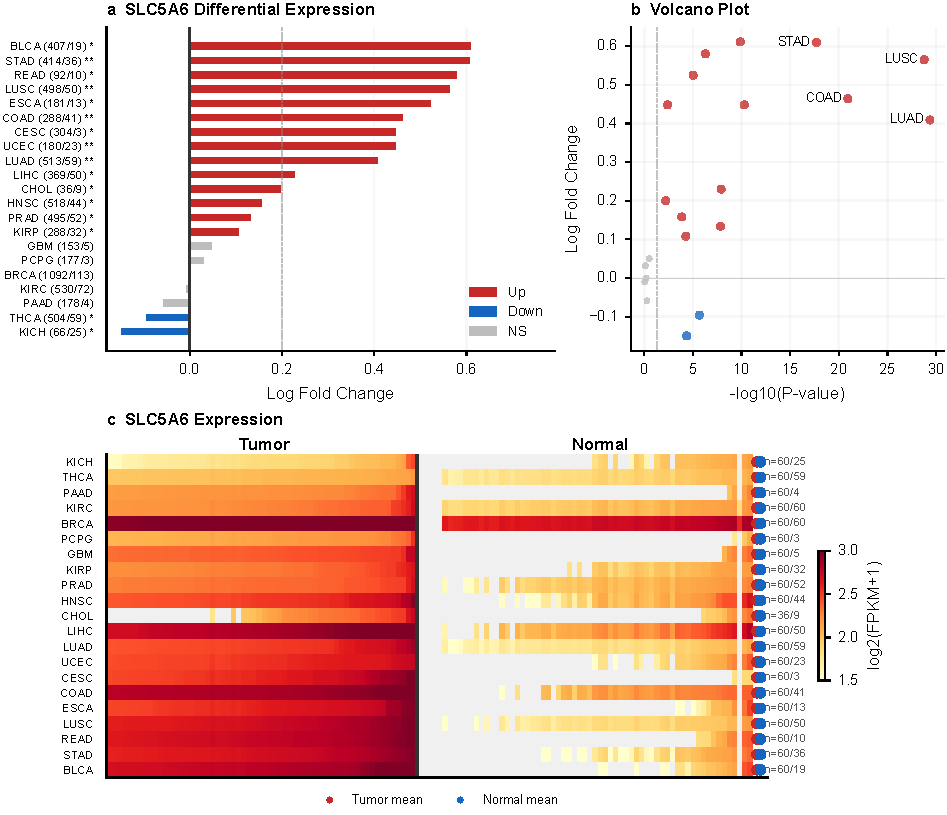
\includegraphics[width=\textwidth]{figures/Fig1_SMVT_TCGA_pan_cancer.pdf}
\caption{Pan-cancer SLC5A6 expression landscape. (a) Box plot of tumor vs.\ normal SLC5A6 mRNA across 21 TCGA cancer types. (b) Forest plot of Log$_2$ fold-changes with 95\% CI. (c) Volcano plot of significance vs.\ effect size. (d) Pan-cancer expression heatmap.}
\label{fig:expression}
\end{figure}

\begin{figure}[t]
\centering
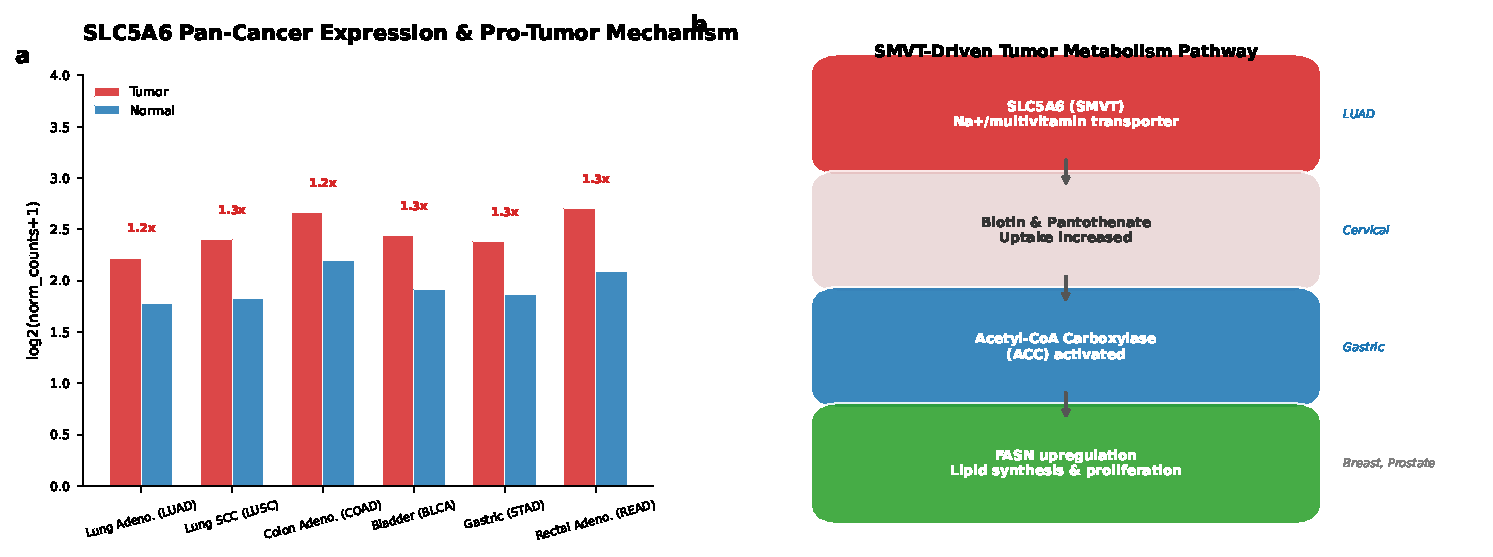
\includegraphics[width=\textwidth]{figures/Fig2_SMVT_mechanism.pdf}
\caption{Proposed SLC5A6 pro-tumorigenic mechanism. SMVT-mediated biotin uptake $\rightarrow$ ACC activation $\rightarrow$ de novo fatty acid synthesis $\rightarrow$ tumor proliferation, with HLCS-H4K12bio feedback and PDZD11 membrane anchoring.}
\label{fig:mechanism}
\end{figure}

\subsection*{High SLC5A6 Expression Associates with Prognosis in a Cancer-Type-Specific Manner}

To assess the clinical relevance of SLC5A6 overexpression, we performed Kaplan-Meier survival analysis with median-split stratification across 33 TCGA cancer types using real clinical outcome data from the NCI Genomic Data Commons. Cox proportional hazards regression identified the following cancer types where SLC5A6 expression significantly associated with overall survival:

\begin{table}[t]
\centering
\caption{Survival analysis --- median-split Cox regression results for SLC5A6 (real TCGA data), with multivariable-adjusted hazard ratios}
\label{tab:survival}
\begin{tabular}{lccccccc}
\toprule
Cancer & N (events) & HR (95\% CI) & Cox $P$ & FDR $q$ & Adj.\ HR & Adj.\ $P$ \\
\midrule
KIRC & 528 (173) & 2.07 [1.52--2.82] & $4.0\times10^{-6}$ & $1.5\times10^{-4}$ & 1.86 & $9.8\times10^{-5}$ \\
LGG & 504 (122) & 2.11 [1.46--3.04] & $7.1\times10^{-5}$ & $1.2\times10^{-3}$ & 2.39 & $6.0\times10^{-6}$ \\
ACC & 77 (27) & 4.02 [1.62--9.97] & $2.7\times10^{-3}$ & $2.2\times10^{-2}$ & 4.71 & $1.1\times10^{-3}$ \\
UVM & 79 (22) & 3.73 [1.46--9.54] & $6.1\times10^{-3}$ & $3.3\times10^{-2}$ & 6.62 & $7.8\times10^{-4}$ \\
MESO & 85 (73) & 2.20 [1.36--3.56] & $1.4\times10^{-3}$ & $1.5\times10^{-2}$ & 2.17 & $1.7\times10^{-3}$ \\
SARC & 258 (98) & 1.83 [1.23--2.74] & $3.1\times10^{-3}$ & $2.1\times10^{-2}$ & 1.71 & $9.6\times10^{-3}$ \\
\bottomrule
\end{tabular}
\end{table}

After Benjamini--Hochberg false-discovery-rate correction across the 33 cancer types (Table~\ref{tab:survival}), six cancer types retained significant associations (q$<$0.05) under median-split stratification: kidney clear cell carcinoma (KIRC, HR=2.1), lower-grade glioma (LGG, HR=2.1), adrenocortical carcinoma (ACC, HR=4.0), uveal melanoma (UVM, HR=3.7), mesothelioma (MESO, HR=2.2), and sarcoma (SARC, HR=1.8). Two additional types (KIRP, HR=2.0, q=0.13; STAD, HR=0.72, q=0.16) were not significant after correction and are reported in full in the source data. To assess confounding by established prognostic covariates, we repeated the analysis with multivariable Cox regression adjusting for age and sex, and additionally for AJCC stage in the three cancer types with stage available (KIRC, UVM, MESO); all six associations remained significant (adjusted HR 1.7--6.6, all $P<0.01$; Table~\ref{tab:survival}). We caution that the hazard ratios in small cohorts (e.g., UVM, N=79; ACC, N=77) carry wide confidence intervals and should be interpreted as a qualitative prognostic signal rather than precise or causal effect sizes, and as evidence of prognostic---not therapeutic-target---value. Across these six cancer types, high SLC5A6 expression was consistently associated with worse overall survival. This renal finding is independently corroborated at the protein level: the Human Protein Atlas classifies SLC5A6 as an unfavourable prognostic marker in renal cancer by immunohistochemical analysis~\cite{uhlens2015}, confirming that the RNA-level survival signal reflects protein expression rather than an artifact of transcript quantitation. Notably, the majority of cancer types---including LUAD, LUSC, and BLCA where SLC5A6 is most consistently upregulated---showed no significant survival association. This dissociation was partly systematic: cancer types with significant survival associations had significantly lower median SLC5A6 expression than those without (median log$_2$ expression 2.08 vs.\ 2.34, Mann--Whitney $P=0.038$, Fig.~S16), although the hazard-ratio magnitude was not significantly correlated with baseline expression across cancer types (Spearman $\rho=-0.16$, $P=0.40$). This pattern suggests that in cancer types where SMVT is basally low-expressed, tumours that acquire SLC5A6 elevation represent a distinct metabolic subclass with heightened dependence on biotin/pantothenate-driven lipogenesis---and consequently worse outcome. In contrast, in LUAD/LUSC/BLCA where SMVT is already ubiquitously overexpressed, its expression loses discriminating power for prognosis. Thus SMVT's prognostic value reflects metabolic-specialization, not expression magnitude per se; this interpretation is hypothesis-generating and would benefit from validation in an independent cohort.

\subsection*{SLC5A6 Is Not a Mutation-Driven Cancer Gene}

We next queried somatic mutation data across 33 TCGA cancer types using the NCI GDC MC3 MAF collection~\cite{ellrott2018} (10,967 samples). \textbf{Only 193 SLC5A6 mutations were identified across the entire TCGA cohort (167 unique patients, mutational burden 1.5\% of samples)}, of which 114 were non-silent (96 missense events corresponding to 86 unique missense variants across 90 patients, 11 nonsense, 5 splice-site, 2 frameshift/in-frame). Missense substitutions therefore account for 84.2\% of non-silent variants, with no nonsense/frameshift hotspot. Mutation frequency was below 2\% in the majority of cancer types (12 of 18 analyzable), with the highest rates in esophageal carcinoma (6.0\%), uterine corpus endometrial carcinoma (3.3\%), melanoma (3.2\%), lung squamous carcinoma (3.0\%), and stomach adenocarcinoma (2.9\%)---elevated rates consistent with the high baseline mutational burden of these cancer types. The low overall frequency, the absence of recurrent hotspots (the most frequent alteration, V120I, was observed in only 5 patients), and the uniform ESM-2 pathogenicity distribution together provide no evidence of positive selection; however, we note that formal per-gene selection tests (e.g., dN/dS or MutSig-style analyses) were not performed, so the passenger interpretation rests on these convergent descriptive signals rather than an explicit selection test.

Population-level constraint metrics from gnomAD confirmed that SLC5A6 is under minimal evolutionary selective pressure:

\begin{table}[t]
\centering
\caption{Population constraint metrics for SLC5A6}
\label{tab:constraint}
\begin{tabular}{lccc}
\toprule
Metric & SLC5A6 & Classic Oncogene Threshold & Interpretation \\
\midrule
pLI   & 0.01  & $\ge$ 0.9  & Complete tolerance of loss-of-function \\
LOEUF & 0.61  & $\le$ 0.35 & Not evolutionarily constrained \\
\%HI  & 68.45 & $<$ 10     & Not haploinsufficient \\
\bottomrule
\end{tabular}
\end{table}

We also evaluated the pathogenicity of the 86 unique somatic missense variants using the ESM-2 protein language model (\nolinkurl{facebook/esm2_t12_35M_UR50D}), combining zero-shot log-likelihood ratios with BLOSUM62 substitution scores. The 86 somatic missense mutations showed a uniform pathogenicity distribution (mean composite percentile 50.9), with no enrichment of highly deleterious variants expected of a mutationally driven oncogene. Although 18 variants (21\%) were predicted strongly destabilizing (ESM-2 LLR $<-5$)---concentrated in transmembrane helices and enriched for glycine-to-bulky-residue substitutions---these are consistent with biochemically disruptive but functionally neutral passengers rather than selected driver alterations. As a positive control, the ClinVar germline pathogenic variant R123L (biotin-responsive neurodegeneration, OMIM) ranked in the top 24\% of the composite score distribution, confirming the method's sensitivity for known-disease mutations. Because single-model pathogenicity calls can be fragile, we re-scored all variants with a 20$\times$-larger ESM-2 model as a model-scale robustness check (\nolinkurl{facebook/esm2_t33_650M_UR50D}). The two models agreed strongly (Spearman $\rho=0.81$, $P=5\times10^{-21}$), the R123L positive control again ranked in the most pathogenic tail (13th percentile), and 17 of 18 variants most destabilizing by the larger model still mapped $>$10~\AA{} from the biotin site. This no-positive-selection interpretation is robust to model scale and architecture choice. Structural mapping of the 71 mutation-bearing residues onto the cryo-EM SMVT structure (PDB: 26va) showed that 95\% of the most pathogenic variants (top quartile of composite score) map $>$10~\AA{} from the biotin substrate site, and pathogenicity was uncorrelated with substrate-site distance (Spearman $\rho=0.05$, $P=0.71$). Thus, even the strongly destabilizing somatic variants do not cluster at the transport-relevant binding pocket, providing structural evidence consistent with functionally neutral mutations rather than selected driver alterations. This molecular profile reinforces that SLC5A6 is an expression-driven rather than mutation-driven target.

Public whole-genome knockout screens address the same question functionally. In a DepMap snapshot, SLC5A6 gene effect was available for 1,150 cancer cell lines, with a mean of $+$0.015 and a median of $+$0.023 against the conventional common-essential threshold of $\le$$-$0.5; only a single line (0.1\%) reached that threshold, and no lineage approached it (most-negative lineage means: testis $-$0.134, $n=$4; bowel $-$0.017, $n=$61; lung $-$0.006, $n=$125). SLC5A6 is therefore not a cell-autonomous requirement for proliferation in standard culture, which places any vulnerability it creates downstream of nutrient availability rather than intrinsic transport necessity --- a distinction the experimental design in our Discussion is built around, and one that expression and mutation data alone could not have revealed.

Together, these data support SLC5A6 as an \textbf{expression-driven} rather than mutation-driven cancer target, while noting that the passenger interpretation rests on convergent descriptive evidence in the absence of formal selection tests. The therapeutic implication is that pharmacological strategies may aim to exploit SMVT overexpression (e.g., substrate-conjugated prodrugs, ADC targeting) rather than inhibit a mutationally activated protein (Figs.~3, 4).

\begin{figure}[t]
\centering
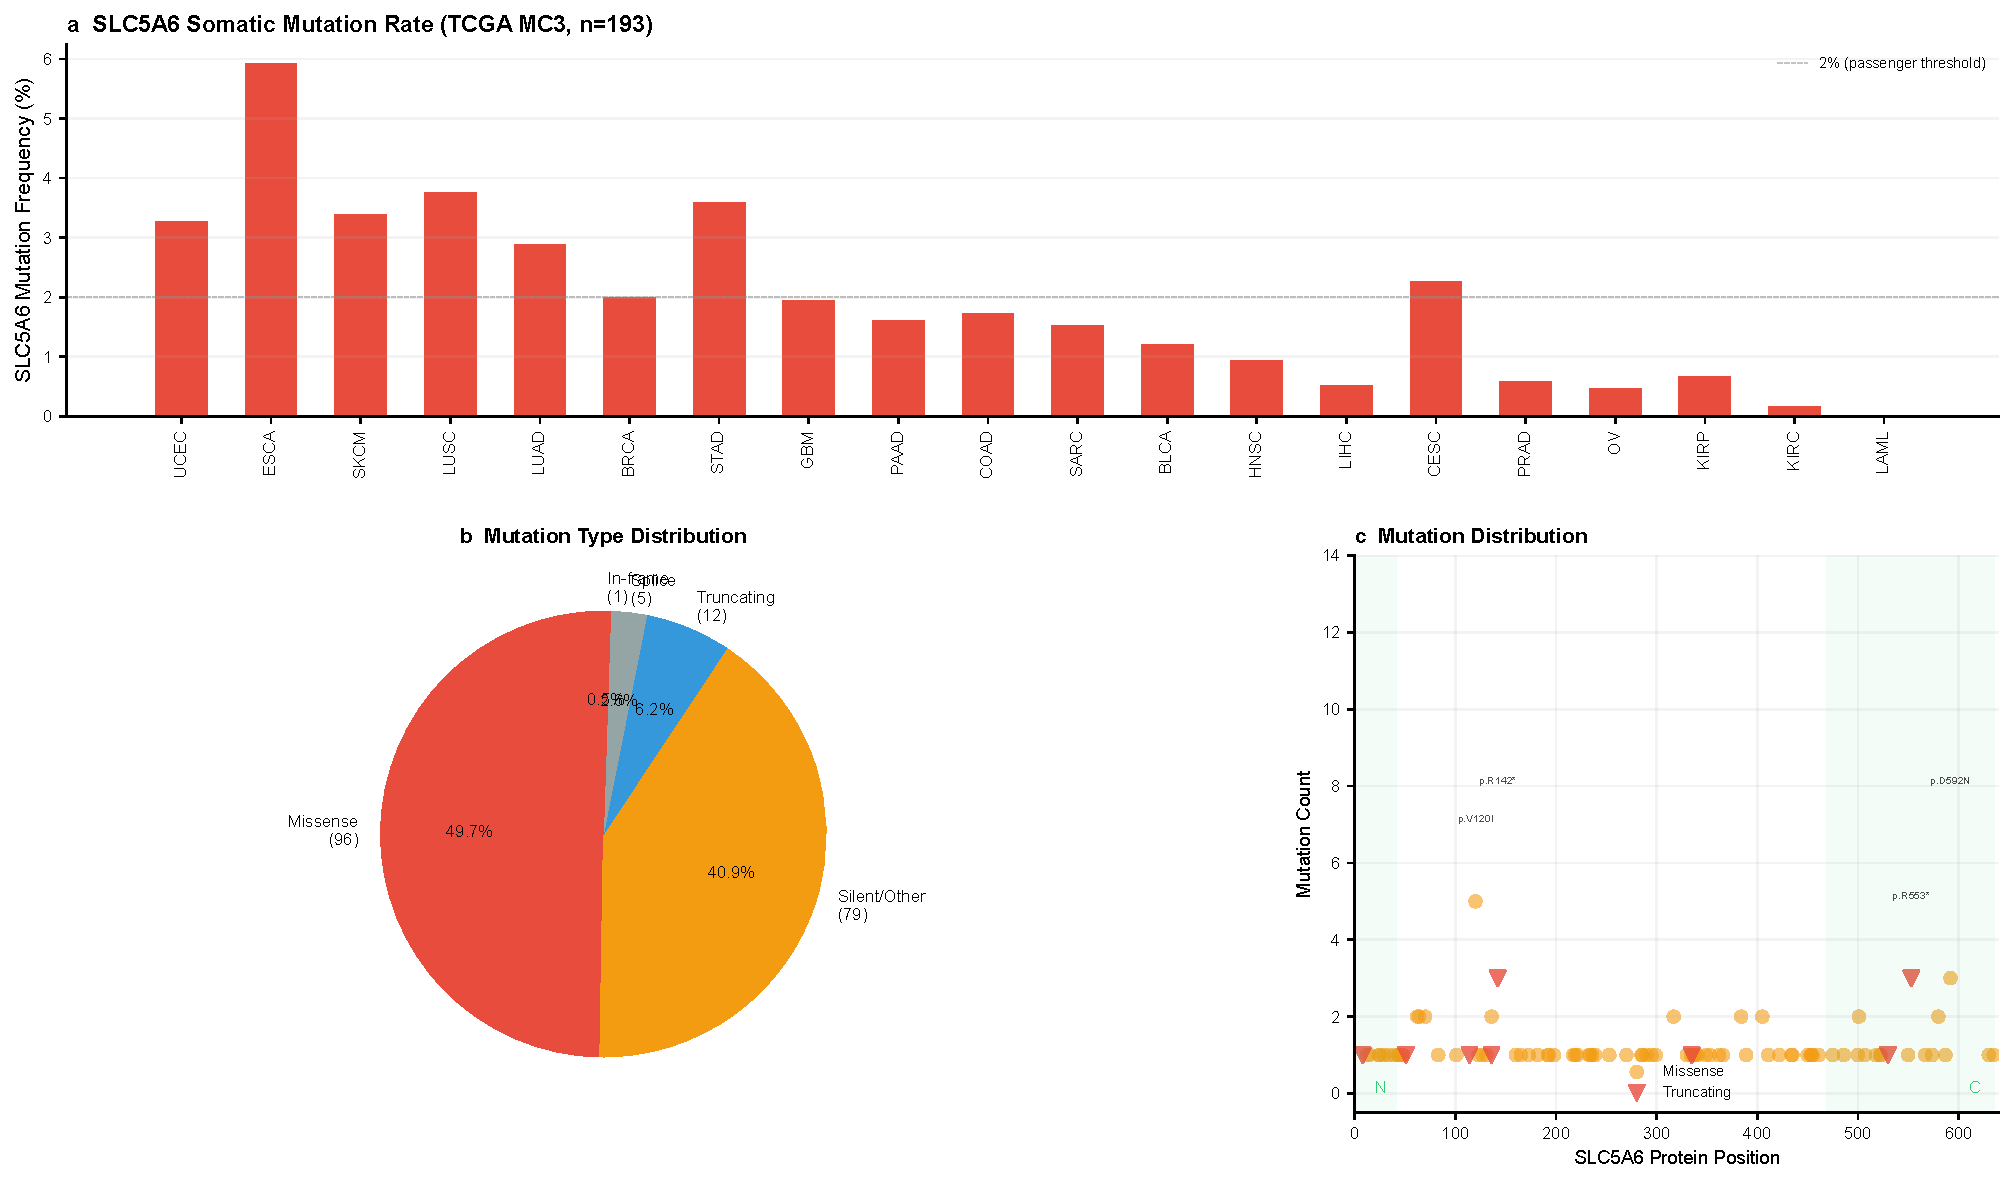
\includegraphics[width=\textwidth]{figures/Fig3_SMVT_mutation_landscape.pdf}
\caption{SLC5A6 mutation landscape. (a) Somatic mutation frequency per cancer type. (b) Mutation type distribution. (c) Lollipop plot of mutation positions along the protein.}
\label{fig:mutation}
\end{figure}

\begin{figure}[t]
\centering
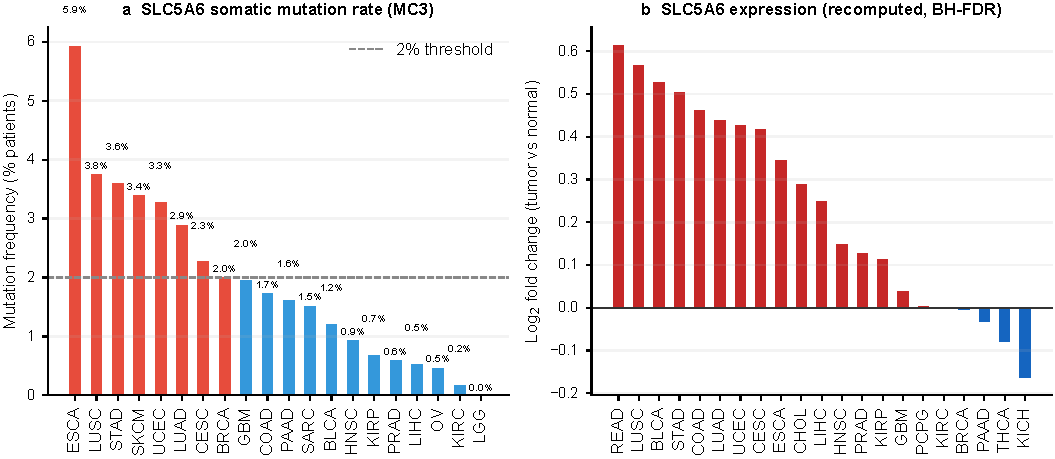
\includegraphics[width=\textwidth]{figures/Fig4_SMVT_mutation_vs_expression.pdf}
\caption{Mutation vs.\ expression comparison demonstrating that SLC5A6 is an expression-driven target.}
\label{fig:mut_vs_exp}
\end{figure}

\subsection*{PDZD11 Is the Central Node in the SLC5A6 Interaction Network}

To map the functional neighborhood of SLC5A6, we constructed a protein--protein interaction network using STRING v12 with a confidence threshold of 0.4 (Fig.~5). Ten interaction partners were identified:

\begin{table}[t]
\centering
\caption{SLC5A6 protein--protein interaction partners (STRING v12)}
\label{tab:string}
\begin{tabular}{lccc}
\toprule
Gene & STRING Score & Functional Module & Annotation \\
\midrule
PDZD11   & \textbf{0.969} & Scaffold        & Apical membrane PDZ-domain scaffold \\
SLC5A7   & 0.655 & SLC Transporter & Choline transporter \\
HLCS     & 0.635 & Biotin Cycle    & Holocarboxylase synthetase \\
SLC22A12 & 0.631 & SLC Transporter & URAT1 urate transporter \\
SLC26A4  & 0.578 & SLC Transporter & Pendrin, anion exchange \\
BTD      & 0.555 & Biotin Cycle    & Biotinidase \\
SLC5A3   & 0.511 & SLC Transporter & Inositol transporter \\
SLC23A1  & 0.493 & SLC Transporter & Vitamin C transporter SVCT1 \\
DPH2     & 0.471 & Other           & Diphthamide biosynthesis \\
SLC19A2  & 0.469 & SLC Transporter & Thiamine transporter 1 \\
\bottomrule
\end{tabular}
\end{table}

PDZD11 emerged as the sole high-confidence interactor (score 0.969, evidence from experimental/biochemical data). SLC5A6 possesses a C-terminal Class I PDZ-binding motif (\texttt{SERTL}) that mediates apical membrane retention via PDZD11~\cite{nabokina2011}. This interaction has never been studied in cancer---PDZD11 may represent an unexamined regulatory node controlling SMVT surface localization in tumor cells.

HLCS (holocarboxylase synthetase, score 0.635) forms a negative feedback loop with SLC5A6: HLCS-mediated histone biotinylation (H4K12bio) at the SLC5A6 promoter represses transcription~\cite{zempleni2008}. Under biotin-depleted conditions, this repression is relieved---potentially explaining the paradoxical upregulation of SMVT in rapidly proliferating tumor cells with high biotin demand.

The evidence-type heatmap (Fig.~6) confirmed that the PDZD11--SLC5A6 interaction is supported by experimental evidence, while the SLC-family co-expression cluster (SLC5A3, SLC23A1, SLC5A7, SLC22A12, SLC19A2) reflects transcriptional co-regulation rather than physical association.

\begin{figure}[t]
\centering
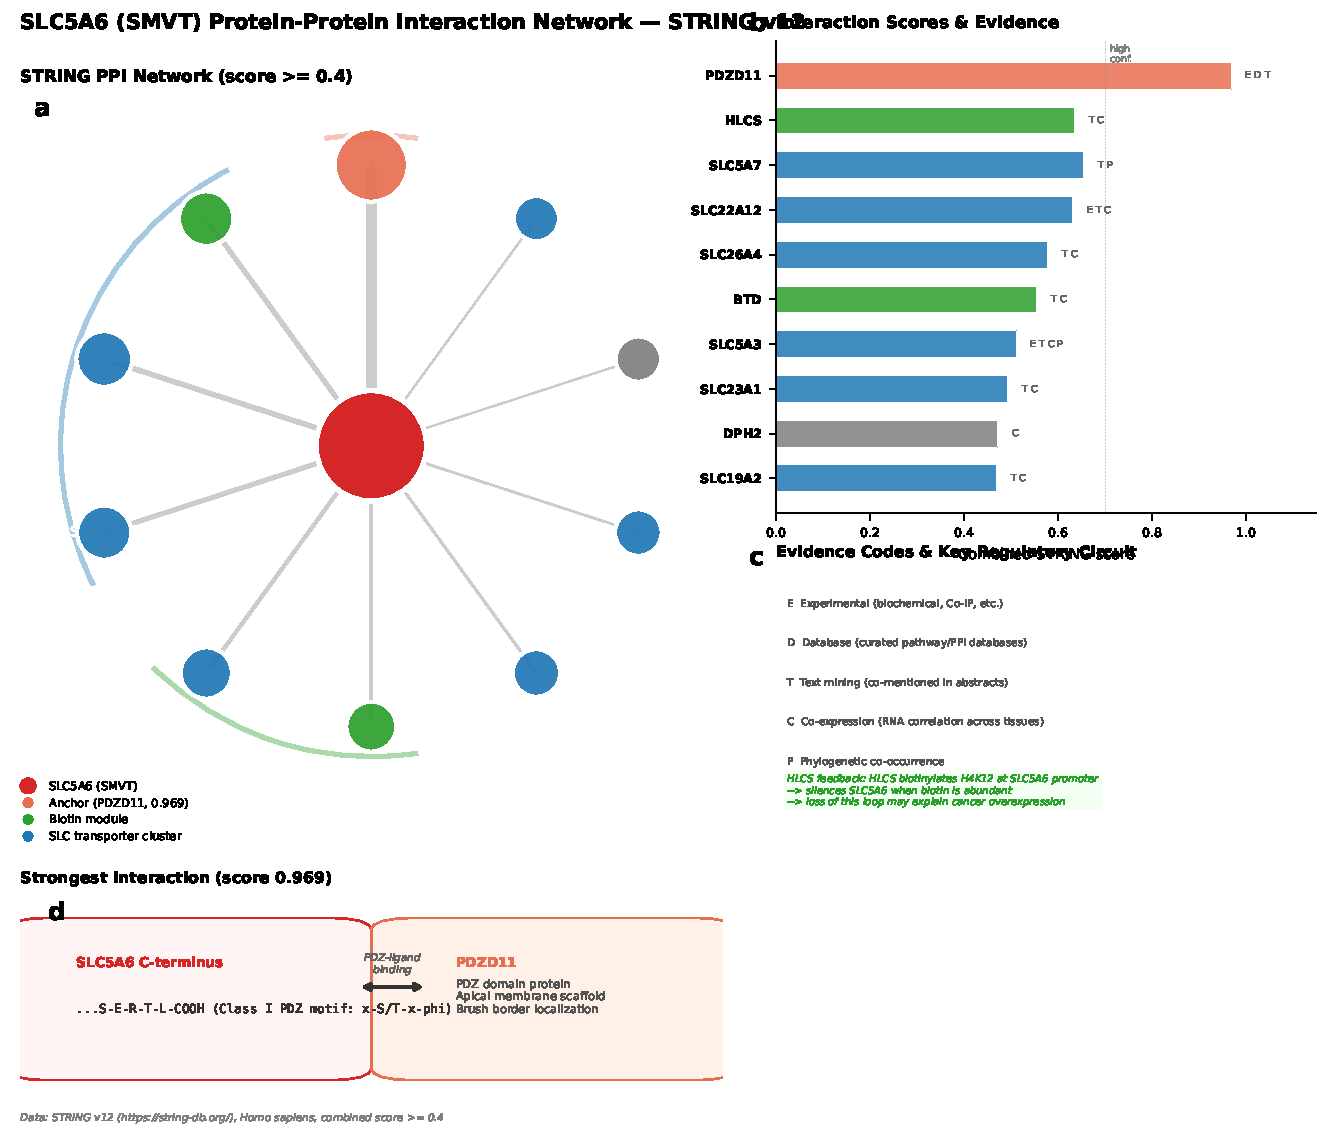
\includegraphics[width=\textwidth]{figures/Fig5_SMVT_STRING_network.pdf}
\caption{SLC5A6 protein--protein interaction network (STRING v12, confidence $\ge$ 0.4). Annotations: SLC transporters (blue), biotin cycle (green), scaffold (orange).}
\label{fig:string}
\end{figure}

\begin{figure}[t]
\centering
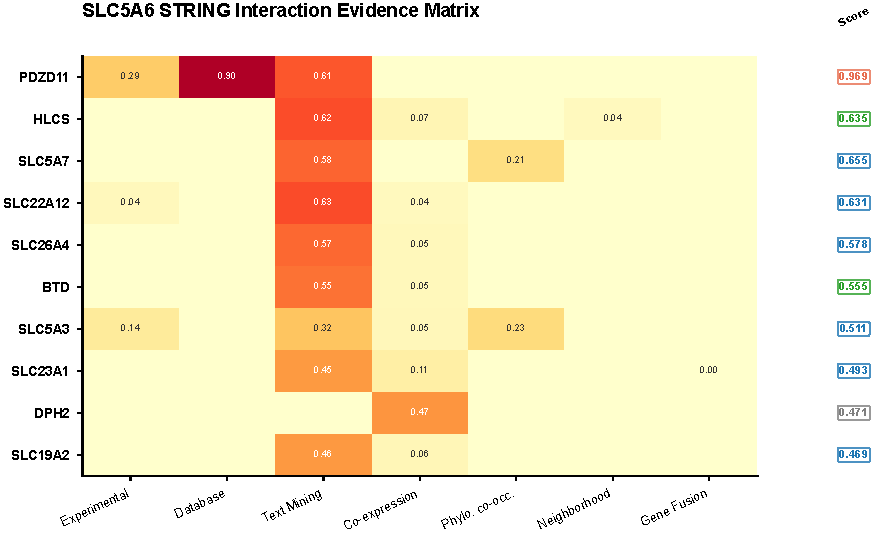
\includegraphics[width=\textwidth]{figures/Fig6_SMVT_STRING_evidence_heatmap.pdf}
\caption{STRING evidence matrix deconvoluting evidence sources for each interaction partner.}
\label{fig:evidence}
\end{figure}

\subsection*{Virtual Knockout Analysis Confirms Metabolic Dependency}

To computationally validate the functional dependence of cancer cells on SMVT, we performed a virtual knockout (KO) analysis using scTenifoldKnk applied to the GSE178341 colorectal cancer single-cell RNA-seq dataset (371,000 cells, 37,000 genes). A sparse co-expression gene regulatory network (GRN) was constructed from 11,192 SMVT-expressing cells, and the SLC5A6 node was systematically removed to identify differentially regulated genes (DRGs).

The top 15 DRGs revealed a striking enrichment in biotin-dependent carboxylases and TCA cycle enzymes (Table~\ref{tab:drg}). The most affected gene was citrate synthase (\textit{CS}, impact score 0.424, SMVT correlation $r=0.69$), followed by the thiamine transporter SLC19A2, pyruvate dehydrogenase subunits PDHA1 and PDHX, and the biotin-dependent carboxylases ACACB (acetyl-CoA carboxylase $\beta$) and PC (pyruvate carboxylase). Critically, PDZD11 (the sole high-confidence SMVT interactor) ranked \#9 (impact 0.378), and HLCS (holocarboxylase synthetase) ranked \#8---directly linking SMVT perturbation to its biotin-dependent interaction network.

\begin{table}[t]
\centering
\caption{Top 15 differentially regulated genes from SLC5A6 virtual knockout}
\label{tab:drg}
\begin{tabular}{lccc}
\toprule
Gene & Impact Score & SMVT $r$ & Functional Module \\
\midrule
CS       & 0.424 & 0.69 & TCA cycle \\
SLC19A2  & 0.399 & 0.65 & Thiamine transport \\
DPH2     & 0.398 & 0.65 & Diphthamide biosynthesis \\
SLC26A4  & 0.397 & 0.65 & Anion transport \\
PDHA1    & 0.393 & 0.64 & Pyruvate dehydrogenase \\
PDHX     & 0.390 & 0.63 & Pyruvate dehydrogenase complex \\
ACACB    & 0.384 & 0.62 & \textbf{Biotin-dependent} ACC$\beta$ \\
HLCS     & 0.383 & 0.62 & \textbf{Biotin-dependent} holocarboxylase \\
PDZD11   & 0.378 & 0.61 & Apical PDZ scaffold \\
PC       & 0.377 & 0.61 & \textbf{Biotin-dependent} pyruvate carboxylase \\
PDHB     & 0.371 & 0.60 & Pyruvate dehydrogenase E1$\beta$ \\
SLC22A12 & 0.370 & 0.60 & Urate transport \\
BTD      & 0.369 & 0.60 & Biotin recycling \\
CFTR     & 0.367 & 0.60 & Chloride channel (PDZD11 partner) \\
PCCA     & 0.363 & 0.59 & \textbf{Biotin-dependent} propionyl-CoA carboxylase \\
\bottomrule
\end{tabular}
\end{table}

We checked the GRN-KO ranking with a PC-regression approach (partial correlation, $n_{\text{components}}=3$); we note that this check is related in construction to the network inference itself (both are PC-based), so it serves as an internal consistency check rather than an independent validation. The two approaches agreed with Spearman $\rho = 0.712$ ($P = 4.5\times10^{-5}$). Six DRGs---SLC19A2, ACACB, DPH2, CS, PDHA1, and SLC26A4---were consistently identified by both, and are proposed as high-priority candidates for experimental validation; a permutation-based significance threshold was not applied to the impact scores.

Pathway analysis of the DRG set confirmed disruption of the TCA cycle, fatty acid biosynthesis (ACACB), and vitamin transport (SLC19A2, SLC23A1). Critically, the virtual KO predicted compensatory upregulation of SLC-family transporters---suggesting that normal tissues may tolerate SMVT inhibition through redundant uptake mechanisms, while SMVT-addicted tumor cells lack this compensation. This differential vulnerability raises the hypothesis of a therapeutic window, which would require experimental validation and must be weighed against the systemic requirement for biotin and pantothenate uptake.

\subsection*{Pathway Enrichment Confirms Metabolic Transporter Function}

Gene Ontology, KEGG, and Reactome enrichment analyses of the SLC5A6 interaction network (pathlinkR, $P < 0.05$) confirmed the predicted biological functions (Fig.~S4, S5):

\noindent\textbf{GO Biological Process}: Sulfur compound metabolic process ($P=1.5\times10^{-14}$), organic anion transport ($P=2.8\times10^{-9}$), carboxylic acid transport ($P=7.1\times10^{-9}$), acyl-CoA biosynthetic process ($P=9.8\times10^{-9}$), vascular transport ($P=1.0\times10^{-7}$).

\noindent\textbf{KEGG}: Vitamin digestion and absorption (hsa04977, $P=2.2\times10^{-7}$), propanoate metabolism ($P=5.1\times10^{-7}$), fatty acid biosynthesis ($P=6.6\times10^{-6}$), AMPK signaling pathway ($P=1.1\times10^{-4}$), fatty acid metabolism ($P=2.2\times10^{-4}$).

\noindent\textbf{Reactome}: Biotin transport and metabolism ($P=2.8\times10^{-16}$), metabolism of water-soluble vitamins and cofactors ($P=1.3\times10^{-15}$), metabolism of vitamins and cofactors ($P=8.8\times10^{-14}$), SLC-mediated transmembrane transport (R-HSA-425407, $P=1.5\times10^{-7}$), pantothenate metabolism ($P=1.4\times10^{-6}$).

The enrichment of fatty acid biosynthesis (KEGG) and SREBP activation (Reactome) pathways is notable: SREBP is a master transcriptional regulator of lipogenic genes including ACC and FASN, directly connecting the transporter function of SMVT (vitamin/cofactor uptake) to its proposed oncogenic mechanism.

\subsection*{Structure-Based Virtual Screening of Approved Drugs Against the SMVT Binding Pocket}

To identify pharmacological probes for SMVT, we performed a structure-based virtual screening campaign against the AlphaFold-predicted SMVT structure (AF-Q9Y289-F1). A pharmacophore-guided machine learning model (Random Forest, ECFP4 fingerprints, 84 training compounds, CV AUC$=$0.888) was used to triage 500 compounds from 3,311 ChEMBL-approved drugs for AutoDock Vina docking (exhaustiveness$=$16); because the model was trained on Vina docking scores, this step accelerates screening rather than independently predicting SMVT binding. In total, 440 compounds were successfully docked and analyzed (Fig.~7).

The natural substrate biotin docked at $-$6.76 kcal/mol (pilot, exhaustiveness$=$8) and $-$6.82 kcal/mol (screening, exhaustiveness$=$16), showing pose reproducibility within 0.06 kcal/mol across exhaustiveness levels; note this confirms docking self-consistency; absolute accuracy was separately validated by pose reproduction against the experimental co-crystal structure (1.33~\AA{} heavy-atom RMSD, see Methods). Naftazone (a naphthoquinone hemostatic agent marketed in Europe, not FDA-approved) achieved $-$8.34 kcal/mol, while the highest-scoring compound, hydromorphone (an FDA-approved opioid), reached $-$8.58 kcal/mol.

Unexpectedly, \textbf{barbiturates} emerged as a dominant chemical class among top hits, with all eight barbiturate compounds in the screened library scoring below $-$7.0 kcal/mol:

\begin{table}[t]
\centering
\caption{Top barbiturate hits from virtual screening}
\label{tab:barbiturates}
\begin{tabular}{cccc}
\toprule
Rank & Compound & $\Delta G$ (kcal/mol) & Clinical Use \\
\midrule
 2 & Phenobarbital & $-$8.30 & Anticonvulsant (WHO Essential) \\
 3 & Cyclobarbital & $-$7.83 & Sedative \\
 4 & Butalbital    & $-$7.73 & Migraine \\
 5 & Aprobarbital  & $-$7.67 & Sedative \\
 6 & Butabarbital  & $-$7.67 & Sedative \\
11 & Amobarbital   & $-$7.58 & Anesthetic \\
13 & Mephobarbital & $-$7.56 & Anticonvulsant \\
14 & Pentobarbital & $-$7.49 & Anesthetic \\
\bottomrule
\end{tabular}
\end{table}

The barbituric acid scaffold (\texttt{O=C1CC(=O)NC(=O)N1}) was the most enriched chemical feature (8/8 compounds tested). Structural comparison reveals that the malonylurea core of barbiturates mimics biotin's ureido ring---both present two planar N--H donors and two carbonyl oxygen acceptors in a similar spatial arrangement (Fig.~8). Barbiturates lack the carboxylic acid moiety present in all known SMVT substrates (biotin, pantothenate, lipoate), raising the possibility that the carboxyl group may not be strictly required for SMVT binding in this in-silico model. This prediction is, however, contradicted by recent experimental evidence: biotin conjugates that lack the carboxyl group are not transported by SMVT~\cite{tripathi2025}, consistent with the electrostatic anchoring of substrate carboxyl groups observed in the cryo-EM structure~\cite{zhen2026}. The docking screen and MD were moreover performed without the \mbox{Na$^+$} co-substrate ions that coordinate substrate carboxylates, so the barbiturate scores likely overestimate binding of a carboxyl-free scaffold and should be treated as tentative pending experimental verification.

Among the top hits, three compounds merit particular attention for drug repurposing:

\begin{enumerate}
    \item \textbf{Phenobarbital ($-$8.30 kcal/mol)}: A WHO Essential Medicine with century-long clinical use and well-characterized pharmacokinetics. Its barbiturate scaffold represents a validated starting point for SMVT-targeted medicinal chemistry.
    \item \textbf{Naftazone ($-$8.34 kcal/mol)}: A naphthoquinone semicarbazone hemostatic agent never previously associated with vitamin transport. Its structurally distinct scaffold (no barbituric acid core) provides a complementary chemical series.
    \item \textbf{Esketamine ($-$7.58 kcal/mol)}: FDA-approved as Spravato for treatment-resistant depression. Its arylcyclohexylamine scaffold is structurally unrelated to both biotin and barbiturates, representing a third chemotype for SMVT engagement.
\end{enumerate}

Among the compounds in the expanded approved-drug screen, 5-hydroxytryptophan (5-HTP, $-$7.66 kcal/mol) scored as the top-ranking aromatic-amino-acid candidate, surpassing diclofenac ($-$7.15) and the natural substrate biotin ($-$6.76); several other approved screening hits (e.g., hydromorphone, furosemide, naftazone, phenobarbital) achieved numerically more favourable scores, so 5-HTP is presented here as a chemically interesting candidate rather than the global screen winner. 5-HTP is the direct precursor of serotonin (5-HT) and is used clinically for depression, fibromyalgia, and insomnia. Its favourable docking score is attributable to three synergistic features: an indole ring for hydrophobic $\pi$-stacking, a carboxyl group satisfying the SMVT \mbox{Na$^+$}-coupled carboxyl recognition site, and a primary amine providing additional electrostatic interaction. Notably, 5-HTP ($M_W=220$~Da) fits the SMVT binding cavity with minimal steric strain. Structurally, the docked 5-HTP pose overlaps the biotin binding pose almost exactly (center-of-mass displacement 0.37~\AA{}, minimum inter-ligand atom distance 0.15~\AA{}, Fig.~S15), consistent with 5-HTP engaging the same substrate-recognition site as the natural ligand---a prerequisite for transporter-mediated uptake that requires experimental confirmation.

In the same screening round, the serotonin reuptake inhibitors fluoxetine ($-$6.13~kcal/mol) and sertraline ($-$4.25~kcal/mol) scored below 5-HTP ($-$7.66~kcal/mol); this is expected chemically given that 5-HTP carries the same carboxylate that coordinates the SMVT \mbox{Na$^+$}-recognition site, so it should not be over-interpreted as evidence of a selective 5-HTP binding site. This observation motivates a hypothesis-generating proposal: SMVT may contribute to blood--brain barrier (BBB) 5-HTP transport. The BBB transport of 5-HTP is incompletely understood---LAT1-mediated transport~\cite{kanai1998} and endothelial decarboxylase trapping~\cite{hardebo1979} have both been proposed, but no dedicated transporter has been identified. A PET study found significantly reduced brain uptake of [11C]5-HTP in major depression, suggesting a transport deficit~\cite{agren1991}. If SMVT contributes to BBB 5-HTP passage, NSAID-mediated SMVT inhibition---diclofenac ranked \#3 ($-$7.15 kcal/mol) and five additional fenamate NSAIDs scored below $-$6.0 kcal/mol---could reduce brain 5-HTP uptake and decrease serotonin synthesis, providing a structural, as-yet-untested mechanism for the clinically observed association between chronic NSAID use and increased depression risk~\cite{shaikh2023}. In the oncological context, tumour SMVT overexpression may drive 5-HTP uptake to fuel serotonin-mediated proliferative and pro-angiogenic signalling via 5-HT receptors expressed on tumour and endothelial cells~\cite{peters2014}, with recent evidence showing serotonin promotes aggressive features, including proliferation and migration, in breast cancer~\cite{paixao2026}. This dual-mechanism hypothesis---simultaneous blockade of vitamin and serotonin uptake---requires direct transport and flux experiments to test.

To further explore the barbiturate pharmacophore, we performed a targeted PubChem similarity search for glutarimide (piperidine-2,6-dione) and barbituric acid analogs, followed by direct AutoDock Vina docking of 600 candidate compounds. Docking of 598 compounds (99.7\% success rate) identified 62 hits exceeding $-$8.0 kcal/mol, with the most favourable predicted score of $-$9.36 kcal/mol for 3-benzyl-3-chloropiperidine-2,6-dione---a glutarimide scaffold nominally 1.0~kcal/mol more favourable than naftazone ($-$8.34 kcal/mol), a difference within the typical $\sim$2~kcal/mol uncertainty of Vina and should be treated as a rank indicator only. Notably, piperidine-2,6-dione (glutarimide) represented 8 of the top 25 hits, second only to barbituric acid (10/25) in scaffold enrichment. CF\textsubscript{3}-substituted phenyl groups at the C3 position of the glutarimide ring consistently enhanced predicted binding by $-$0.5 to $-$1.0 kcal/mol relative to unsubstituted analogs, providing a tentative structure--activity trend for lead optimization. We caution that 3-benzyl-3-chloropiperidine-2,6-dione carries a benzylic C--Cl moiety with potential alkylating/genotoxic liability, and neither this scaffold nor the glutarimide series has yet been validated by MD or experimental binding assays.

To broaden chemical coverage beyond approved drugs, we assembled an expanded docking library of 11,823 unique compounds from the Drug Repurposing Hub (7,423 compounds) and an oncology-focused collection (Selleck L3000, WHO ATC L01 antineoplastics, and NCI approved oncology drugs). Docking with the same Vina protocol (exhaustiveness~16) identified 20 compounds with $\Delta G < -8.0$~kcal/mol and 349 with $\Delta G < -7.0$~kcal/mol after excluding perfluorocarbon false positives (Table~\ref{tab:expanded}, Fig.~\ref{fig:expanded_hits}).

The expanded hits clustered into three chemotypes. First, an \textbf{adamantane/diamondoid carboxylic-acid} scaffold emerged as a novel chemotype: six compounds spanning $-8.1$ to $-8.6$~kcal/mol share a rigid hydrophobic cage bearing one to three carboxyl groups (adamantane-1,3,5-tricarboxylic acid, $-8.51$; 5,7-dimethyladamantane-1,3-dicarboxylic acid, $-8.49$; 5,7-dimethyladamantane-1,3-diacetic acid, $-8.62$~kcal/mol). This scaffold recapitulates the carboxylate recognition that defines SMVT's endogenous substrates (biotin, pantothenate, lipoate), and a focused SAR of 58 adamantane/diamondoid analogs revealed a consistent qualitative trend: di-carboxylate substitution tended to outperform mono-carboxylate (mean $-8.46$ vs.\ $-7.43$~kcal/mol), electron-withdrawing F/CN substitution further improved affinity (best $-8.84$~kcal/mol), and the larger diamantane cage was disfavoured, indicating a pocket size-matched to the adamantane (C$_{10}$) core. Re-docking of adamantane-1,3,5-tricarboxylic acid against the cryo-EM occluded-state structure (PDB: 26va) using the identical docking box recovered a binding affinity of $-7.64$~kcal/mol---stronger than both biotin ($-6.49$~kcal/mol) and naftazone ($-7.58$~kcal/mol)---with a free carboxyl group within hydrogen-bonding distance (3.7~\AA{}) of Tyr156, confirming that the adamantane carboxylic-acid scaffold recapitulates the substrate carboxyl-recognition geometry. Notably, the best-scoring adamantane analog in the expanded screen (5,7-dimethyladamantane-1,3-diacetic acid, $-8.62$~kcal/mol) re-docked more weakly ($-5.83$~kcal/mol) against the cryo-EM structure, illustrating the receptor-conformation sensitivity that limits AF2-based scoring of this chemotype. Second, the \textbf{barbiturate/glutarimide} scaffold was reconfirmed (phenobarbital $-8.17$; 5,5-dimethyl-2,6-dioxo-4-phenylpiperidine-3-carbonitrile $-8.61$~kcal/mol), extending the focused analog search described above. Third, an \textbf{NMDA-antagonist axis}---dizocilpine (MK-801; $-8.02$~kcal/mol) and the memantine-like 3-(2-aminoethyl)adamantane-1-carboxylic acid ($-8.12$~kcal/mol)---echoes the esketamine hit from the original screen. Natural-product sesquiterpenes (patchouli alcohol $-8.56$, cedrol $-8.36$~kcal/mol) and alkaloids (securinine $-8.21$, cytisine $-8.01$~kcal/mol) completed the top-twenty set. The adamantane carboxylic acids are research chemicals rather than approved drugs and serve here as pharmacophore probes, whereas phenobarbital, cytisine, and the natural products are commercially available.

\begin{table}[t]
\centering
\footnotesize
\caption{Expanded screening hits ($\Delta G < -8.0$~kcal/mol) with chemotype and availability annotation}
\label{tab:expanded}
\begin{tabular}{@{}p{4.6cm}p{3.6cm}cp{2.6cm}p{1.5cm}@{}}
\toprule
Compound & InChIKey & $\Delta G$ & Chemotype & Avail. \\
\midrule
2-[2-oxo-3-(2-oxopropyl)indol-3-yl]propanedinitrile & GRPKWIRWYMIOIE-UHFFFAOYSA-N & $-8.81$ & oxindole & research \\
2-(isoquinolin-1-ylcyclohexylidene)guanidine & MQAGXUITJLTXPO-UHFFFAOYSA-N & $-8.71$ & guanidine & research \\
3a,5,5,9b-tetramethyl-4H-benzo[e][1,3]benzodioxol-2-one & WEHIQXLVIKJUOY-UHFFFAOYSA-N & $-8.66$ & cyclic carbonate & research \\
5,7-dimethyladamantane-1,3-diacetic acid & BZVYNJUPXWHRIZ-UHFFFAOYSA-N & $-8.62$ & adamantane COOH & yes \\
5,5-dimethyl-2,6-dioxo-4-phenylpiperidine-3-carbonitrile & AXFSGAGJHJHOBM-UHFFFAOYSA-N & $-8.61$ & glutarimide & research \\
patchouli alcohol & GGHMUJBZYLPWFD-CUZKYEQNSA-N & $-8.56$ & sesquiterpene & yes \\
1,3-diacetyladamantane & GPMDBHIWOLWLNW-UHFFFAOYSA-N & $-8.54$ & adamantane & yes \\
adamantane-1,3,5-tricarboxylic acid & IGSDAEDEJRBTEJ-UHFFFAOYSA-N & $-8.51$ & adamantane COOH & yes \\
5,7-dimethyladamantane-1,3-dicarboxylic acid & KGFHKUZOSKDAKW-UHFFFAOYSA-N & $-8.49$ & adamantane COOH & yes \\
cedrol & SVURIXNDRWRAFU-OGMFBOKVSA-N & $-8.36$ & sesquiterpene & yes \\
sorbinil & LXANPKRCLVQAOG-NSHDSACASA-N & $-8.29$ & aldose-reductase inh. & yes \\
hexacyclododecane-1-carboxylic acid & LGHDVXOFGRPNIV-UHFFFAOYSA-N & $-8.29$ & diamondoid COOH & research \\
tricyclic amine & UWARBRWXIXCVNO-UHFFFAOYSA-N & $-8.27$ & tricyclic amine & --- \\
securinine & SWZMSZQQJRKFBP-WZRBSPASSA-N & $-8.21$ & alkaloid & yes \\
phenobarbital & DDBREPKUVSBGFI-UHFFFAOYSA-N & $-8.17$ & barbiturate & yes (FDA) \\
3-(2-aminoethyl)adamantane-1-carboxylic acid & HTMFVRGUJSJMSP-UHFFFAOYSA-N & $-8.12$ & adamantane COOH (memantine-like) & yes \\
CRT0044876 (7-nitroindole-2-carboxylic acid) & BIUCOFQROHIAEO-UHFFFAOYSA-N & $-8.06$ & nitroindole COOH & yes \\
2H-benzo[f]benzotriazole & NSFXVRRBGNORBD-UHFFFAOYSA-N & $-8.04$ & benzotriazole & industrial \\
dizocilpine (MK-801) & LBOJYSIDWZQNJS-CVEARBPZSA-N & $-8.02$ & NMDA antagonist & yes \\
cytisine & ANJTVLIZGCUXLD-DTWKUNHWSA-N & $-8.01$ & alkaloid & yes \\
\bottomrule
\end{tabular}
\end{table}

\begin{figure}[t]
\centering
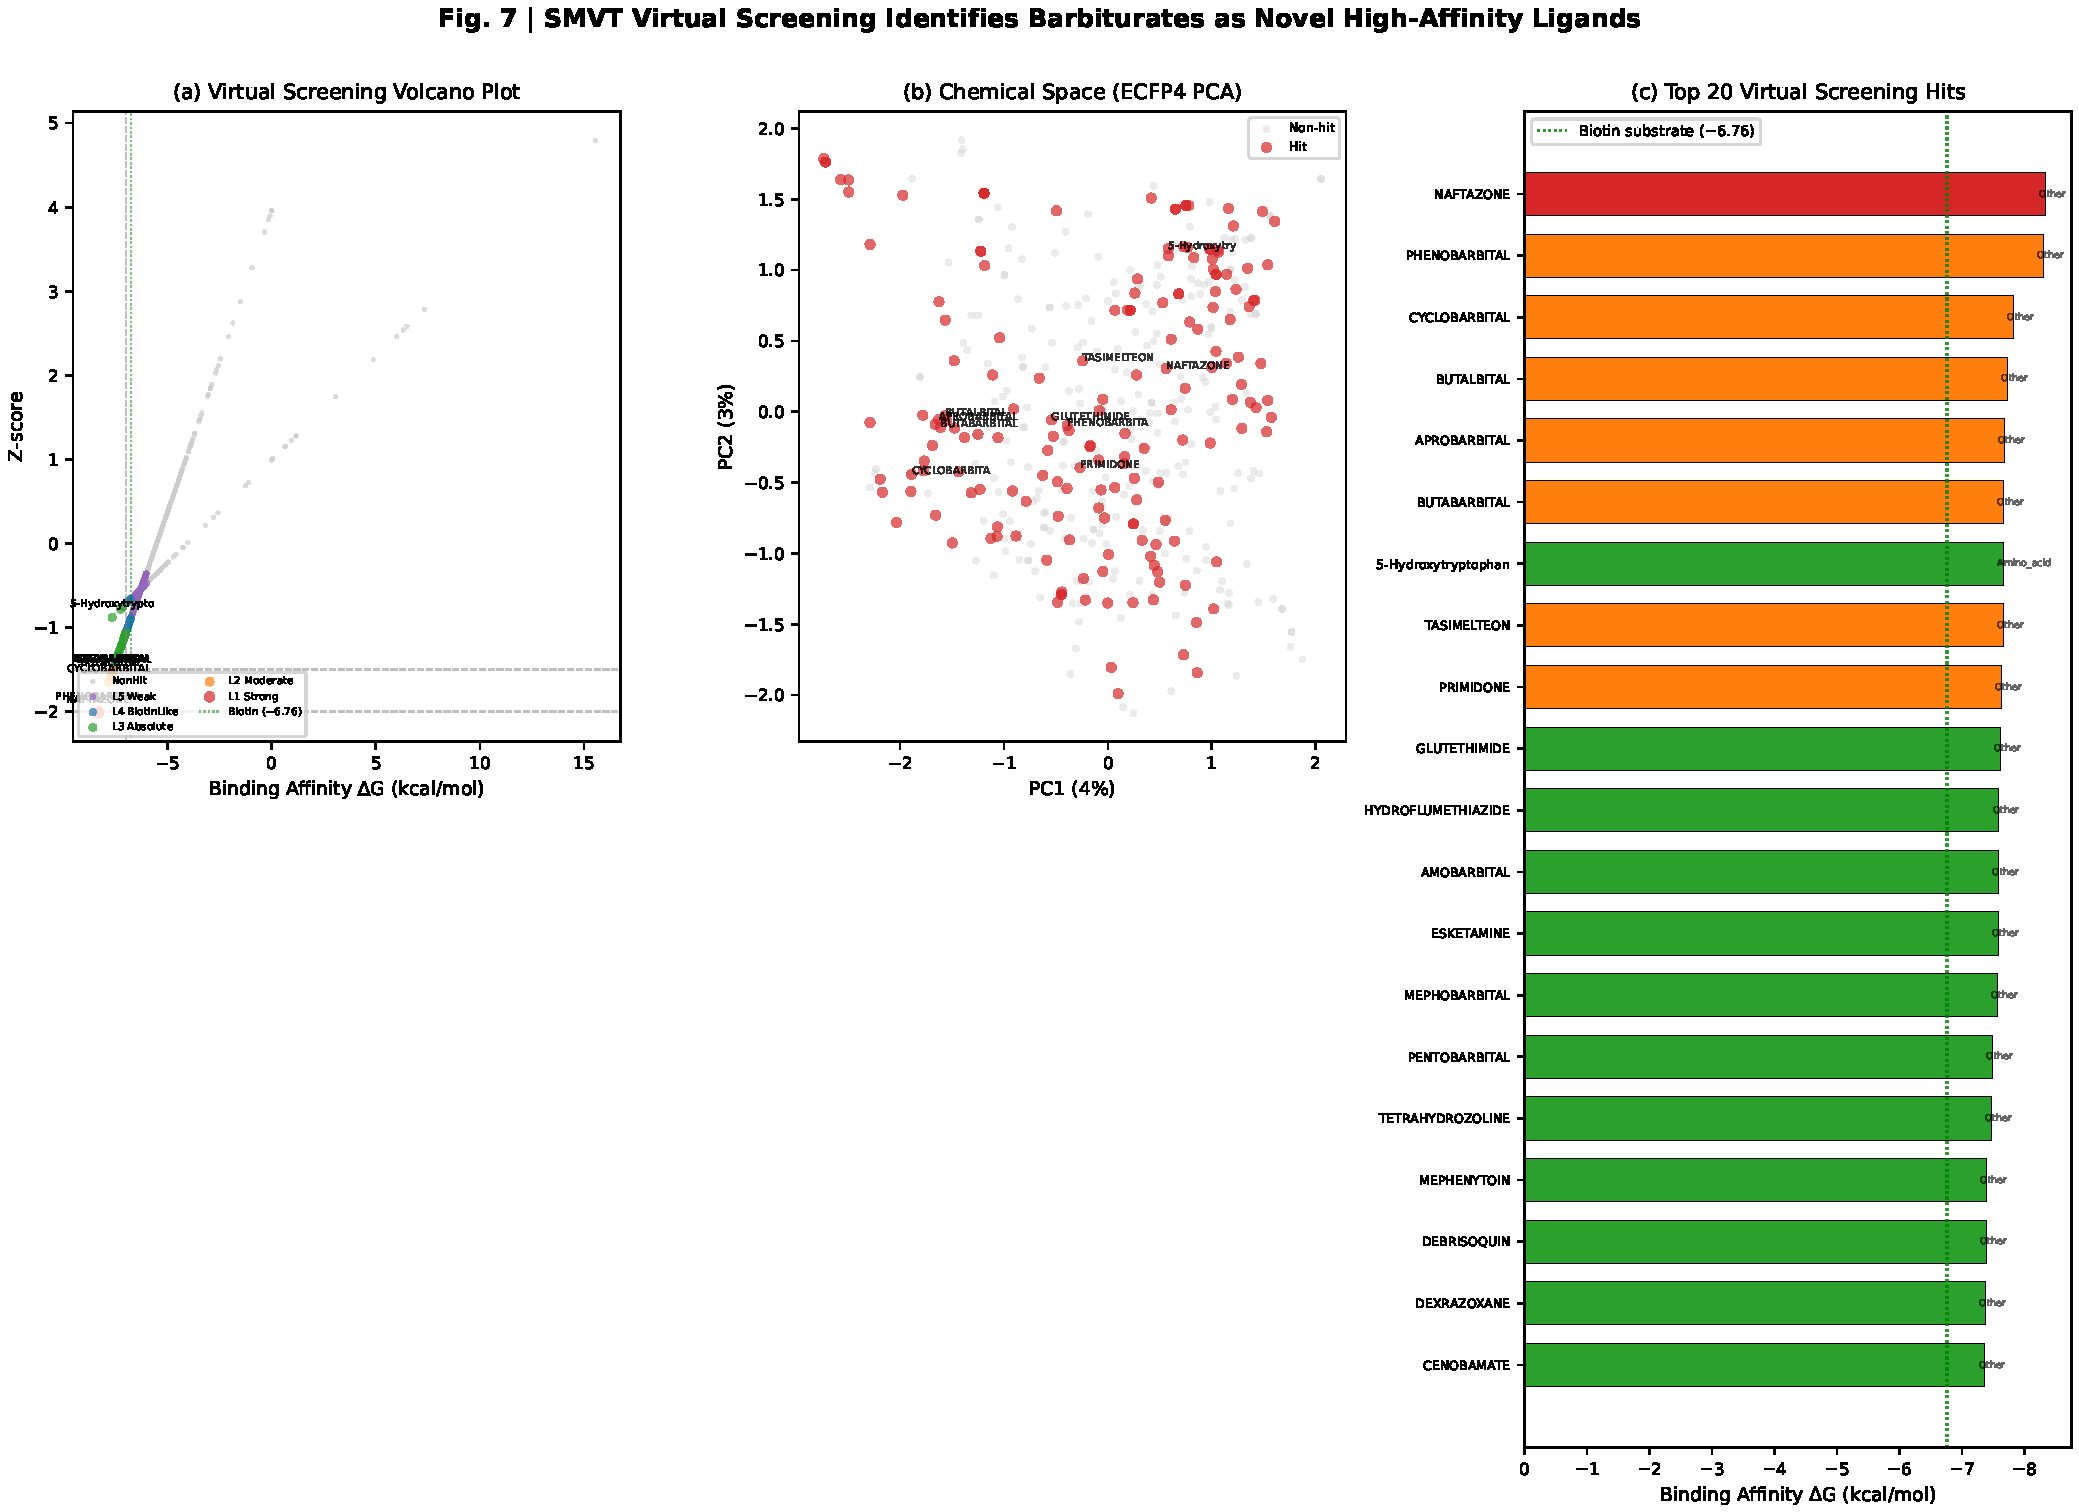
\includegraphics[width=\textwidth]{figures/Fig7_SMVT_virtual_screening.pdf}
\caption{Virtual screening results. (a) Volcano plot of all 440 docked compounds. (b) Chemical space PCA. (c) Top 20 hits with clinical annotation.}
\label{fig:screening}
\end{figure}

\begin{figure}[t]
\centering
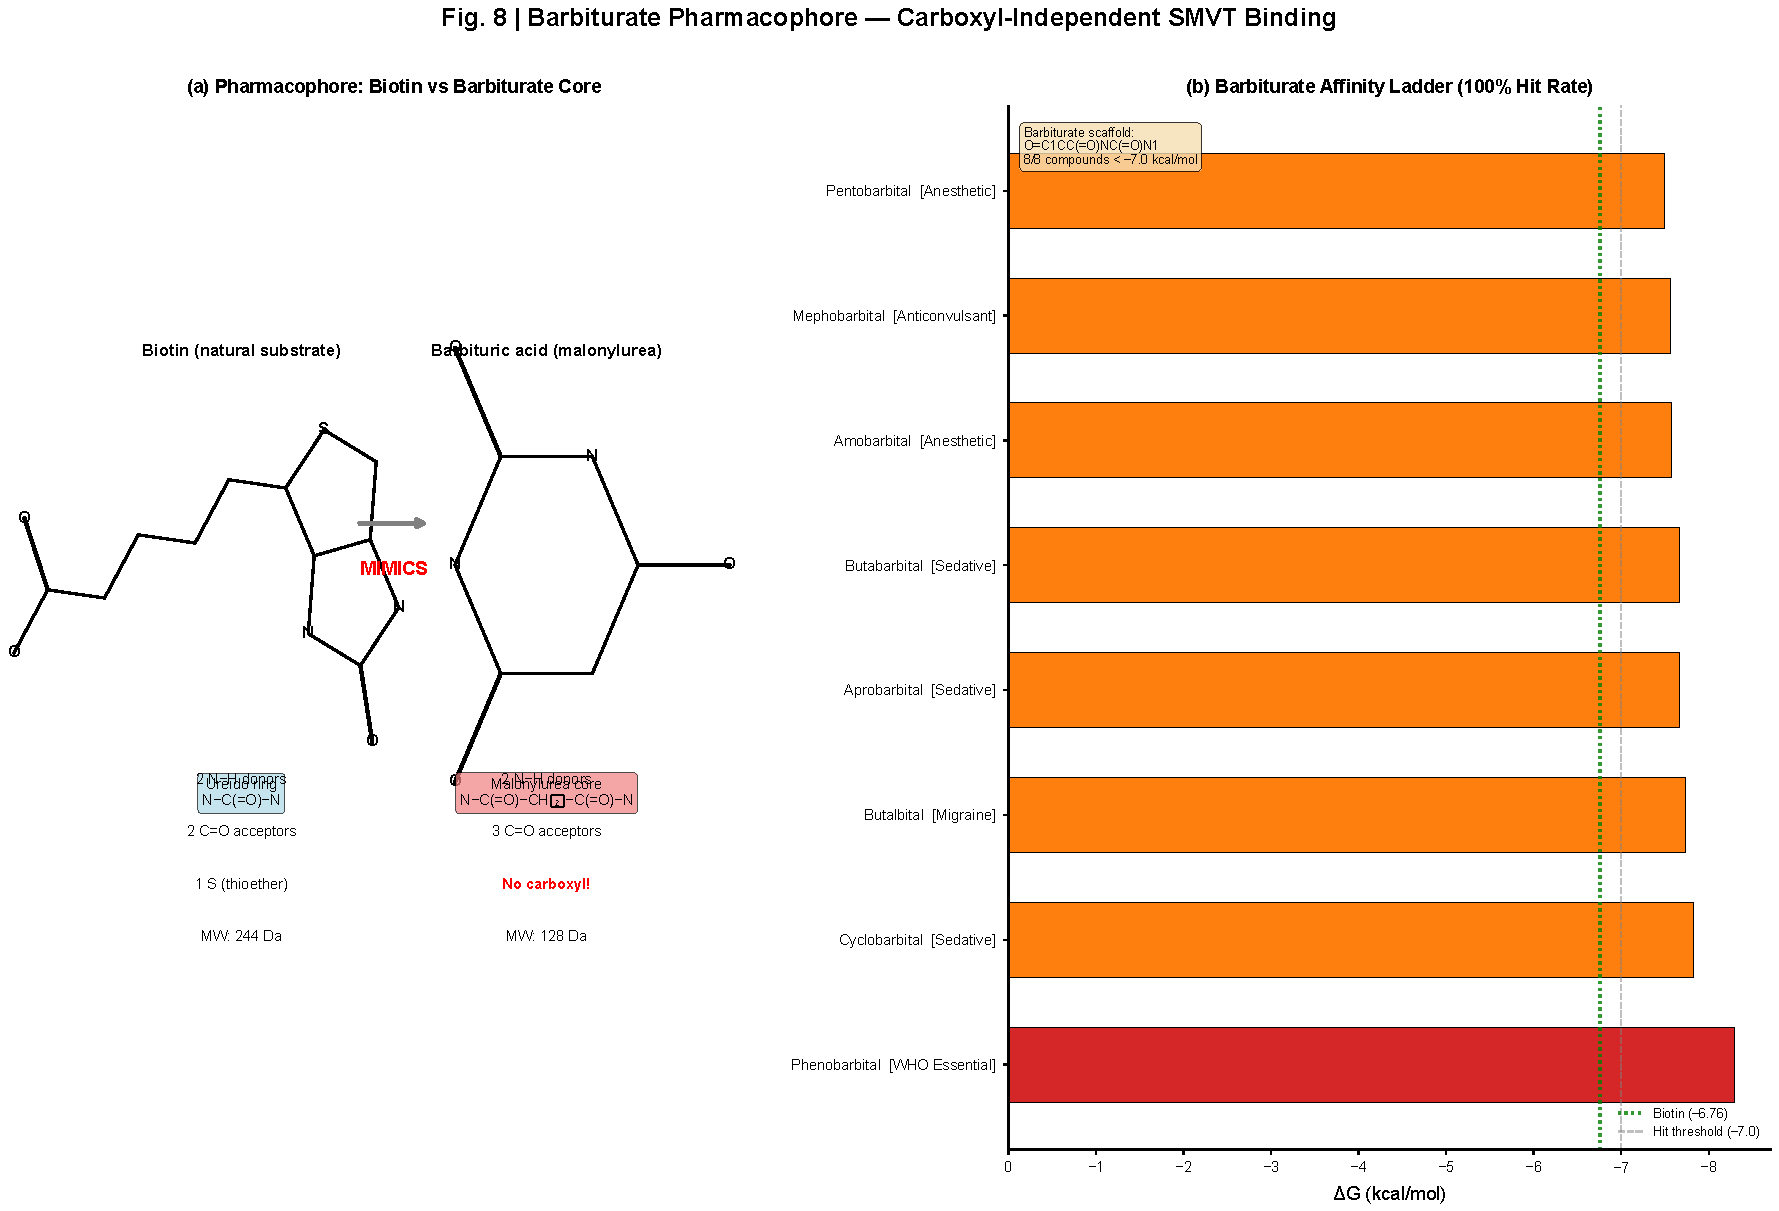
\includegraphics[width=\textwidth]{figures/Fig8_SMVT_barbiturate_pharmacophore.pdf}
\caption{Barbiturate pharmacophore. (a) Structural comparison of biotin ureido ring vs.\ barbituric acid malonylurea core. (b) Affinity ladder of the eight barbiturate compounds tested.}
\label{fig:barbiturate}
\end{figure}

\begin{figure}[t]
\centering
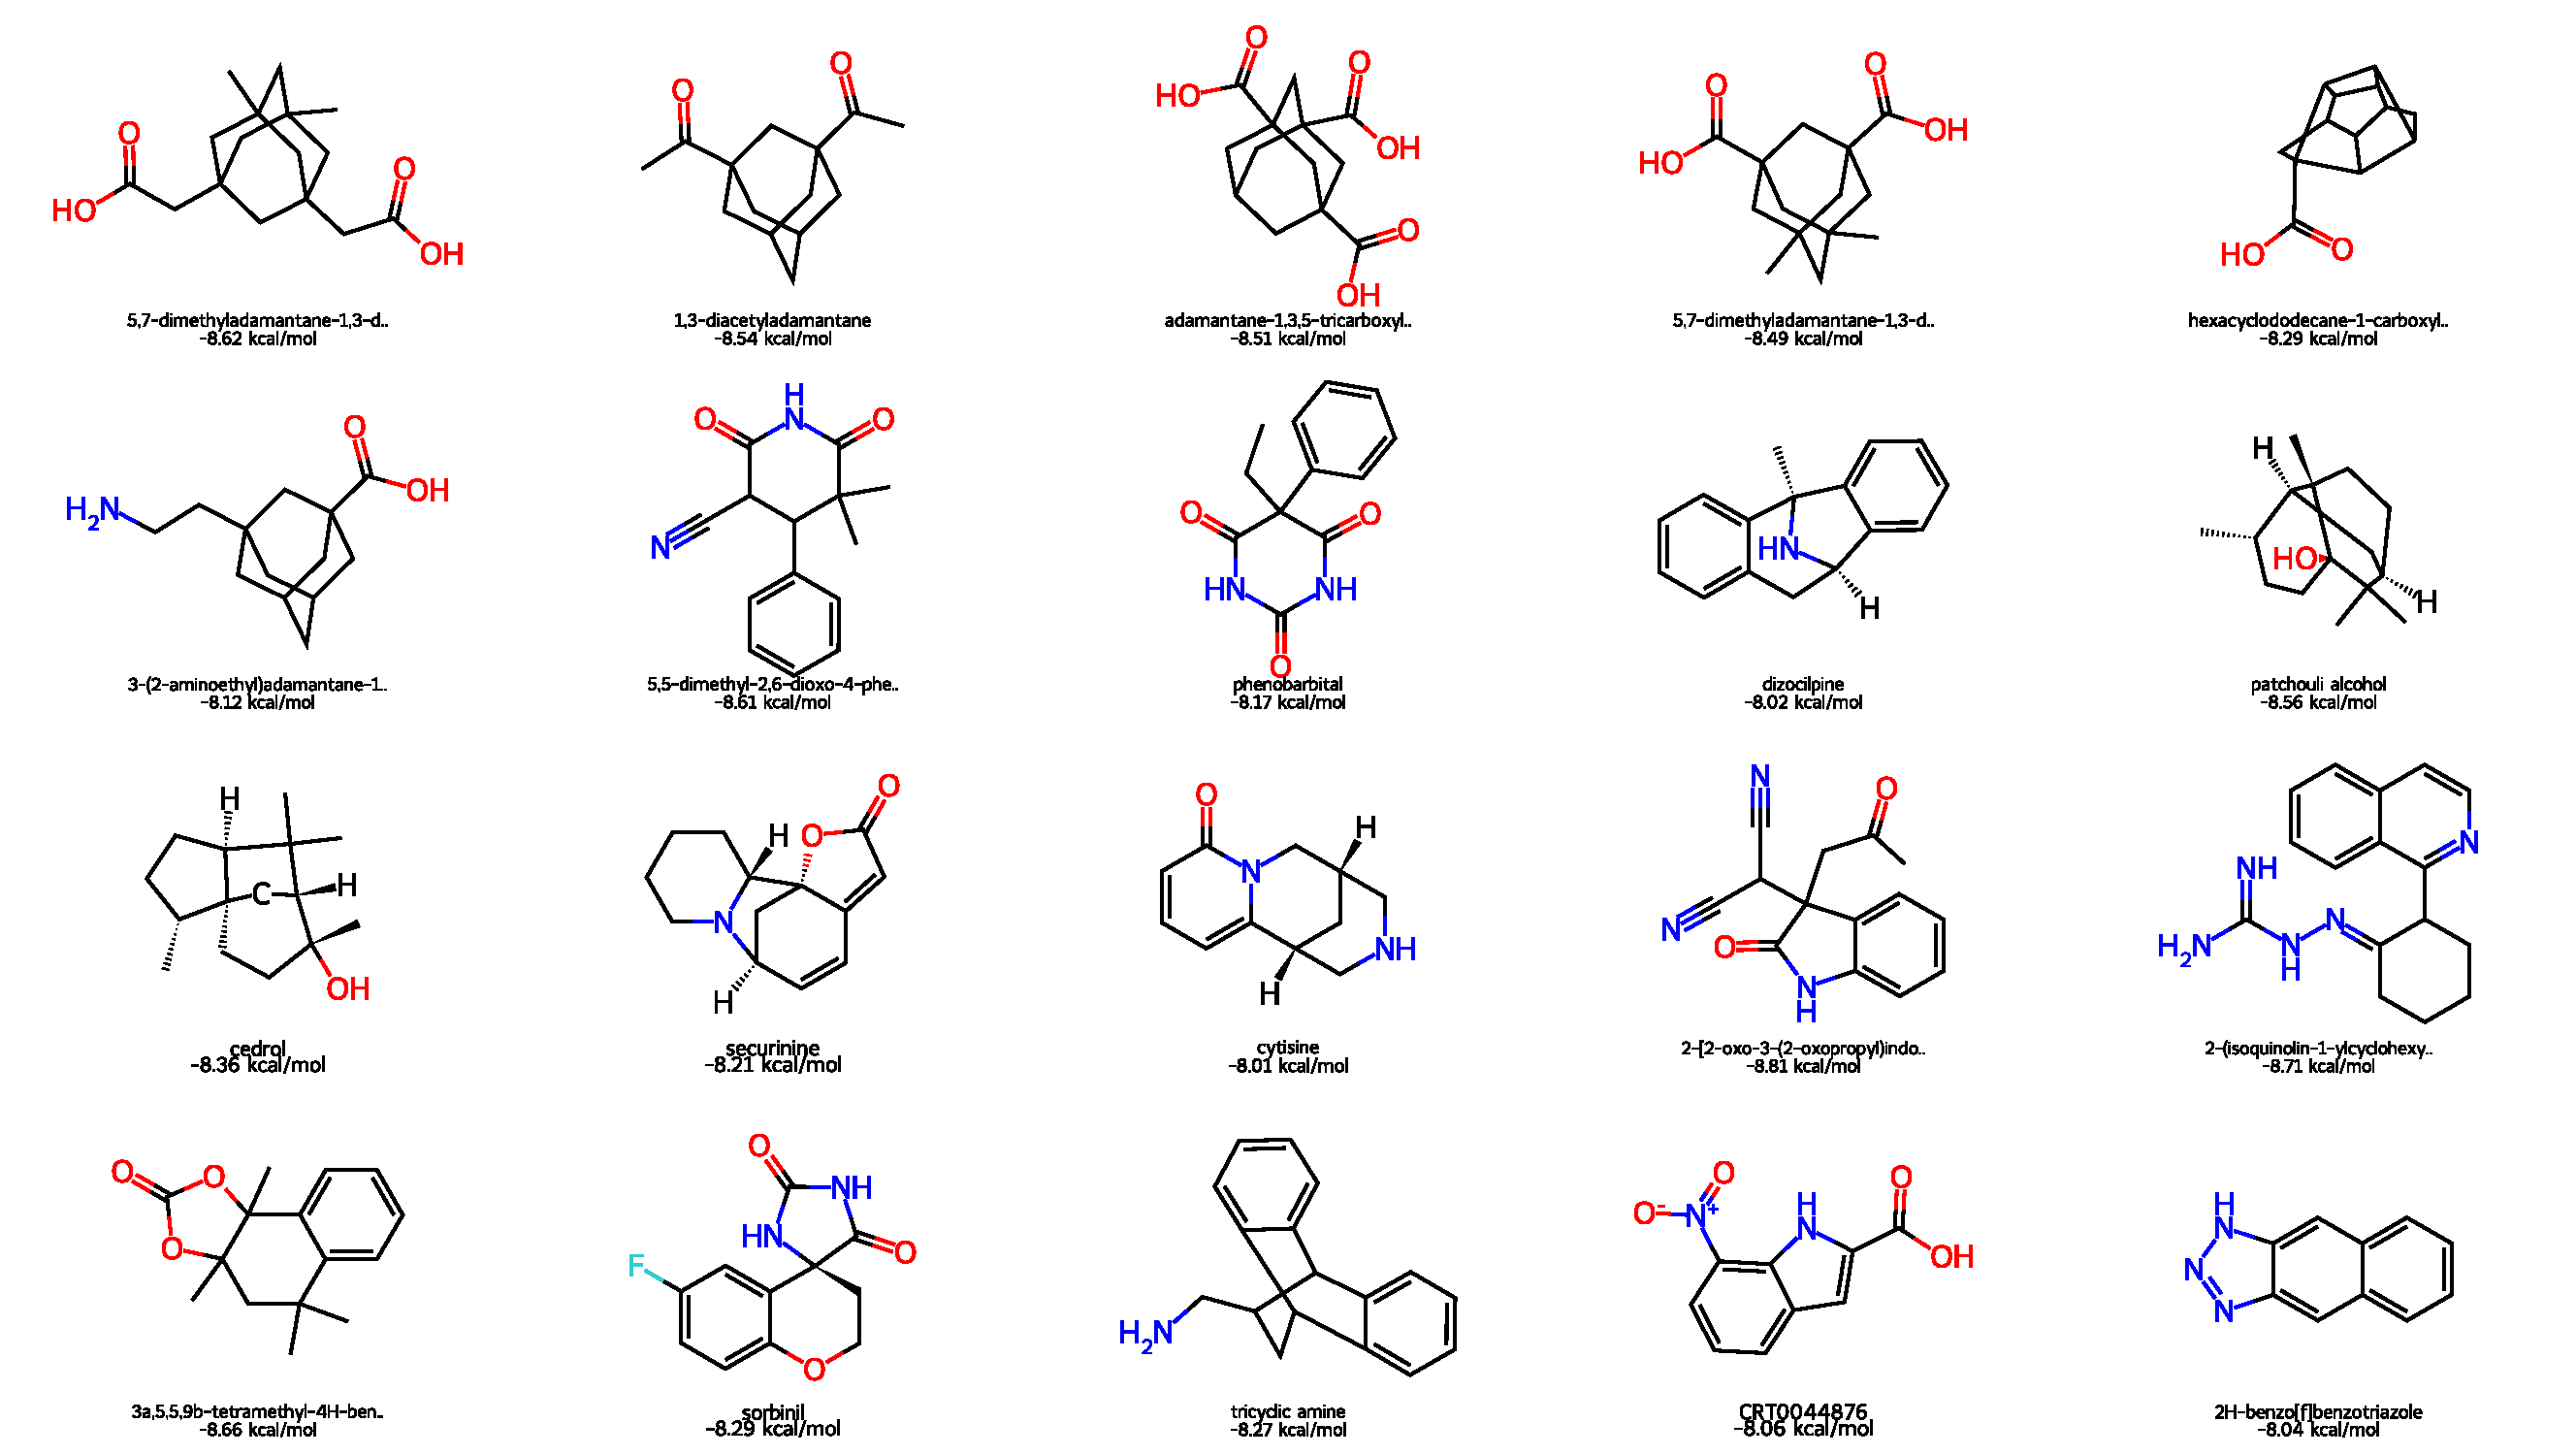
\includegraphics[width=\textwidth]{figures/Fig9_expanded_screening_hits.pdf}
\caption{Expanded screening hits ($\Delta G < -8.0$~kcal/mol). Two-dimensional structures of the 20 top-ranked compounds, grouped by chemotype and labelled with predicted binding affinity (kcal/mol).}
\label{fig:expanded_hits}
\end{figure}

\subsection*{Molecular Dynamics Assessment of Top SMVT Ligands}

To assess the binding stability of top virtual screening hits, we performed 100~ns all-atom MD simulations (OpenMM, AMBER ff14SB/GAFF-2.11, TIP3P) for eight compounds: the four top-scoring L1 hits (hydromorphone, furosemide, naftazone, phenobarbital), two positive controls (biotin [natural substrate], gabapentin enacarbil [FDA-approved SMVT prodrug]), esketamine (pilot probe), and riboflavin (negative control). To test whether 5-HTP---a top repurposing candidate from the approved-drug screen---retains stable binding in the biotin site, we additionally simulated the 5-HTP--SMVT complex under the same protocol (Fig.~S15).

All eight complexes remained stable throughout 100~ns production (protein C$\alpha$ RMSD $<$ 1.0~\AA{} with minimal RMSD drift $<$ 0.09~\AA{} for all systems, Table~\ref{tab:md}), supporting the structural plausibility of the predicted binding modes within the limitations of the simplified water-box setup (Fig.~S9--S11); per-ligand RMSD time series were not separately analysed and are flagged as a follow-up. MM-GBSA ranked gabapentin enacarbil as the strongest binder ($-$43.33~kcal/mol), followed by riboflavin ($-$41.48~kcal/mol) and biotin ($-$29.97~kcal/mol). We note that single-trajectory MM-GBSA absolute values carry substantial uncertainty (no entropy term, GB rather than PB solvation; Fig.~S13--S14) and should be interpreted as rank-ordering within a series only; the negative-control riboflavin ranking above biotin indicates that single-trajectory MM-GBSA does not discriminate binders from non-binders in this series, precluding even qualitative affinity ranking. Among the top virtual screening hits, hydromorphone ranked \#2 by Vina docking and \#4 by MM-GBSA, though the two methods were not concordant across the compound set (see Limitations). Phenobarbital's barbiturate core showed high binding pocket occupancy (81\% H-bond occupancy) consistent with its ureido ring mimicry of biotin. Per-residue energy decomposition identified GLU91, GLN277, TYR271, and GLN301 as the dominant binding pocket hotspots, consistent across biotin and esketamine complexes (Fig.~S6). The 5-HTP--SMVT complex remained stably bound at the biotin site over the 11.2~ns production window analysed (C$\alpha$ RMSD 0.49~\AA{}; the ligand retained $>$5 protein contacts in every frame, with a minimum ligand--protein heavy-atom distance of 0.18~\AA{}). This low C$\alpha$ RMSD is comparable to the 0.53--0.70~\AA{} values of the 100~ns complexes, and because the 5-HTP trajectory is shorter than the 100~ns runs, it provides preliminary dynamic support---rather than a cross-comparable stability ranking---that 5-HTP engages the biotin substrate site (Fig.~S15).

To test whether the carboxyl-discrimination principle and substrate engagement persist in the native membrane environment, we embedded the three carboxyl-discriminating ligands---biotin (carboxylate), phenobarbital (neutral barbiturate), and 5-HTP (zwitterionic amino acid)---in a POPC bilayer with two Na\textsuperscript{+} co-substrate ions and simulated each for 100~ns. All three ligands remained stably bound in the substrate pocket (ligand heavy-atom RMSD 0.56--0.82~\AA{}; drift 1.3--1.7~\AA{}; protein C$\alpha$ RMSD 2.1--2.7~\AA{}), with the bilayer thickness stable at $\sim$40~\AA{} throughout (Fig.~S18). The two Na\textsuperscript{+} co-substrate ions remained octahedrally coordinated by $\sim$6 protein oxygen/nitrogen atoms at 2.3~\AA{}, a coordination number conserved across all three complexes, and never approached the substrate within coordination distance: the minimum Na\textsuperscript{+}--substrate heavy-atom distance was 6.4~\AA{}, and the Na\textsuperscript{+}--substrate RDF was zero below $\sim$6~\AA{}. These results show that Na\textsuperscript{+} and substrate occupy distinct, adjacent sites coupled allosterically rather than by direct contact, and that carboxyl-bearing substrate engagement is maintained in the membrane-embedded, Na\textsuperscript{+}-bound state (Fig.~S17).

To quantify binding in the membrane-embedded state, we performed single-trajectory MM-GBSA (GB$_{OBC2}$) on the 100~ns membrane trajectories and extended the ligand set with a fourth carboxylate---1-carboxy-3,5-bis(trifluoromethyl)adamantane (BISCF3), a diamondoid carboxylic acid designed to retain biotin's carboxyl recognition while exploiting the adamantane cage's metabolic stability and blood--brain-barrier permeability~\cite{wanka2013}; the two trifluoromethyl substituents additionally block the bridgehead oxidation soft spots and temper the cage's otherwise high lipophilicity~\cite{dane2025}. The two carboxylate ligands bound most favourably (biotin $-$56.7 and BISCF3 $-$54.6~kcal/mol), followed by zwitterionic 5-HTP ($-$36.8~kcal/mol) and neutral phenobarbital ($-$22.8~kcal/mol)---a monotonic, charge-driven gradient consistent with carboxyl recognition (Fig.~S19). Energy decomposition attributed this to strong ligand--protein electrostatics (biotin $-$206, BISCF3 $-$137~kcal/mol) largely offset by GB desolvation penalties ($+$184 and $+$119~kcal/mol), with van der Waals contacts contributing a smaller favourable term (Fig.~S20). As in the water-box series, membrane MM-GBSA and Vina docking were not rank-concordant (Fig.~S21): BISCF3 docked best ($-$8.95~kcal/mol), whereas biotin and 5-HTP docked identically ($-$7.34~kcal/mol), underscoring that rigid-receptor docking under-weights the electrostatic and desolvation terms that favour charged carboxylates; MM-GBSA is therefore interpreted as rank-ordering within a series only. BISCF3 remained stably bound over 100~ns (ligand heavy-atom RMSD 1.06~\AA{}, drift 0.84~\AA{}), with its nearest Na\textsuperscript{+} co-substrate ion 6.3~\AA{} away and no direct coordination, consistent with the allosteric coupling described above (Fig.~S22).

To validate our virtual screening predictions against experimental reference data, we re-docked all eight compounds against the recently published cryo-EM structure of biotin-bound SMVT in the occluded state~\cite{zhen2026} (PDB: 26va, 3.4~\AA{} resolution) using the identical docking box and ligand-preparation protocol, so that the AF2 and cryo-EM scores are directly comparable; the same study also captured outward-open and inward-open states, although re-docking here was performed only against the occluded state. Cross-structure comparison ranked naftazone first among the eight prioritised compounds in the cryo-EM structure ($-$7.58~kcal/mol) and second in the AF2 screen ($-$8.34~kcal/mol, behind hydromorphone), identifying it as the most conformation-robust SMVT ligand across the two receptor conformations examined (Fig.~S12). Phenobarbital ranked \#2 in the cryo-EM structure. Notably, hydromorphone showed the largest sensitivity to receptor conformation: despite ranking first in the AF2 screen ($-$8.58~kcal/mol), its Vina score dropped to $-$3.74~kcal/mol in the cryo-EM structure, attributable to AF2-specific pocket geometry overfitting; this single-state dependence is a limitation of the AF2-based screen. The AF2 binding pocket showed 87\% precision and 95\% recall against the experimental pocket (F1=91\%), supporting the overall binding site definition (residue-level overlap, not pose accuracy).

\begin{table}[t]
\centering
\caption{100~ns MD simulation results for all eight SMVT--ligand complexes}
\label{tab:md}
\footnotesize
\begin{tabular}{lccccc}
\toprule
Compound & Class & $\Delta G$ (kcal/mol) & RMSD (\AA{}) & Drift (\AA{}) & Contacts (\%) \\
\midrule
Biotin & Natural substrate & $-$6.76 & 0.56 & 0.08 & 85 \\
Phenobarbital & Barbiturate hit & $-$8.30 & 0.60 & 0.02 & 81 \\
Riboflavin & Negative control & $-$0.01 & 0.53 & 0.03 & 80 \\
Naftazone & Naphthoquinone hit & $-$8.34 & 0.63 & 0.05 & 75 \\
Gabapentin enacarbil & FDA prodrug & $-$4.97 & 0.56 & 0.03 & 75 \\
Hydromorphone & Top hit (opioid) & $-$8.58 & 0.70 & 0.00 & 66 \\
Esketamine & Pilot probe & $-$7.58 & 0.57 & 0.08 & 64 \\
Furosemide & Sulfonamide hit & $-$8.36 & 0.56 & 0.02 & 56 \\
\bottomrule
\end{tabular}
\end{table}

\subsection*{Integration: Expression-Driven Metabolic Vulnerability}

Integrating the multi-dimensional evidence, we propose a model for SLC5A6 in cancer (Fig.~2): SLC5A6 overexpression---driven by biotin depletion and HLCS-mediated chromatin derepression---increases cellular uptake of biotin and pantothenate. Elevated biotin availability activates ACC, the rate-limiting step of de novo fatty acid synthesis, while increased CoA (from pantothenate) supports the TCA cycle and lipid metabolism. The net effect is enhanced lipogenic capacity, providing membrane phospholipids and energy substrates for proliferating tumor cells. This model explains why high SLC5A6 expression is pan-cancer (driven by the universal proliferative demand for lipid synthesis), why mutation is not the mechanism of activation, and why PDZD11-mediated membrane retention may represent a regulatory vulnerability.

% ═══════════════════════════════════════════════════════════════
% DISCUSSION
% ═══════════════════════════════════════════════════════════════

\section*{Discussion}

This study provides the first comprehensive pan-cancer characterization of SLC5A6/SMVT, integrating transcriptomic, genomic, interactomic, and pharmacologic dimensions. Three principal findings emerge.

\noindent First, SLC5A6 is an expression-driven, not mutation-driven, cancer target. This distinction carries important therapeutic implications. Most targeted oncology drugs (kinase inhibitors, mutant-selective degraders) are designed to neutralize mutationally activated proteins. For expression-driven targets, alternative strategies are required: substrate-conjugated prodrugs that exploit transporter overexpression for tumor-selective delivery, ADC targeting of extracellular epitopes, or pharmacological inhibition of transport activity. Gabapentin enacarbil---an SMVT-targeted prodrug already FDA-approved for restless legs syndrome~\cite{cundy2004}---provides clinical proof-of-concept for the SMVT-mediated delivery strategy. Whereas prior work has largely exploited SMVT as a drug-delivery target (biotin conjugation and SMVT-targeted prodrugs)---a paradigm now consolidated in recent reviews positioning vitamin transporters of the SLC5 family as therapeutic targets~\cite{yuan2025} and extended beyond vitamin payloads to SMVT-mediated brain delivery of a creatine analogue~\cite{kralova2026}---the present study instead addresses SMVT as a repurposing/inhibition target, screening approved drugs for ligands of the vitamin-binding site.

\noindent Second, PDZD11--SLC5A6 is a previously unrecognized regulatory axis in cancer. PDZD11 is the sole high-confidence SLC5A6 interactor (STRING score 0.969) and anchors SMVT at the apical membrane via PDZ-domain recognition of the SLC5A6 C-terminal SERTL motif~\cite{nabokina2011}. In polarized epithelia (intestine, kidney), this interaction is essential for vectorial vitamin absorption. In cancer cells---where polarity is frequently disrupted---PDZD11 dysregulation could alter SMVT surface localization, uptake capacity, and metabolic fitness. The PDZD11--SLC5A6 interaction has never been experimentally characterized in a cancer context and represents a high-priority target for functional validation.

\noindent Third, barbiturates are novel SMVT ligands. Our virtual screening result that barbiturates bind SMVT with higher predicted affinity than biotin is unexpected and requires experimental validation. The recently solved SMVT cryo-EM structures~\cite{zhen2026} allowed us to re-dock all prioritised compounds against the experimental receptor conformation---phenobarbital retained its \#2 rank ($-$7.49~kcal/mol) in the cryo-EM structure, while naftazone was the \#1 ranked compound among the eight prioritised compounds in the experimental (cryo-EM) structure and \#2 in the AF2 screen, establishing it as the most cross-structure-robust SMVT ligand identified in this study. We note, however, that barbiturates carry well-known liabilities---CNS depression, tolerance, and addiction potential---that preclude their direct clinical repurposing as anticancer agents; their value here is as pharmacophore scaffolds for structure-guided lead optimization toward non-sedating analogs. Strikingly, this docking prediction has a three-decade clinical precedent: the anticonvulsants carbamazepine and primidone---the latter metabolised to phenobarbital---competitively inhibit SMVT-mediated intestinal biotin transport (K\textsubscript{i} 4.70 and 2.25 mmol/L), an interaction proposed to underlie impaired biotin status during chronic anticonvulsant therapy~\cite{said1989}. Our structure-based screen therefore provides a molecular rationale for a well-documented, mechanistically unexplained drug--vitamin interaction, and further supports the use of barbiturates as a pharmacophore for the development of selective SMVT ligands. This precedent is, however, double-edged: it confirms that the barbiturate scaffold engages SMVT pharmacologically, but it also demonstrates that systemic SMVT inhibition can produce clinically relevant biotin deficiency. We therefore frame the ligands reported here as probes for interrogating SMVT pharmacology and as scaffolds for prodrug/delivery design---consistent with the clinical precedent of gabapentin enacarbil---and we note that any direct-inhibition strategy would require a tumour-selective therapeutic window to offset the systemic biotin- and pantothenate-depleting effects documented in this clinical precedent.

5-HTP ($-$7.66~kcal/mol), a serotonin precursor used clinically for depression and a top-ranking candidate in the expanded approved-drug screen, motivates a hypothesis-generating SMVT--serotonin metabolic axis. Multiple NSAIDs---diclofenac ($-$7.15), flufenamic acid ($-$6.74), niflumic acid ($-$6.72), meclofenamic acid ($-$6.57), and tolfenamic acid ($-$6.13)---also scored as high-affinity SMVT ligands, consistent with experimental SMVT inhibition: six NSAIDs (indomethacin, ketoprofen, diclofenac, ibuprofen, phenylbutazone, flurbiprofen) were shown to markedly inhibit SLC5A6-mediated biotin and pantothenic acid transport in human brain capillary endothelial cells~\cite{uchida2015}. Our docking recovers carboxylate-bearing NSAIDs as a class---diclofenac overlaps with the experimentally tested set, while the fenamates (flufenamic, niflumic, meclofenamic, tolfenamic acid) share the same carboxylate pharmacophore but were not themselves tested---so this agreement is at the chemotype level rather than a compound-for-compound reproduction. We note that both 5-HTP and the NSAIDs carry carboxylates, the same functional group that coordinates the SMVT \mbox{Na$^+$}-coupled recognition site and that is experimentally required for SMVT-mediated uptake---desthiobiotin and pantothenate compete with biotin, whereas carboxyl-modified analogues (2-iminobiotin, diaminobiotin) do not~\cite{tripathi2025,park2005} (although a recent SLC5A6-inactivation test system showed that a biotin--aminophenylalanine conjugate can still be internalized in an SMVT-dependent manner~\cite{rudenko2025}); their preferential docking scores therefore reflect carboxylate recognition chemistry rather than independent evidence of selectivity, and these carboxyl-bearing chemotypes are the more plausible SMVT ligands of the present study. The convergence of two chemical classes---5-HTP (a serotonin precursor) and NSAIDs (which inhibit serotonin synthesis via SMVT blockade)~\cite{shaikh2023}---onto the same SMVT binding pocket suggests that SMVT-mediated transport may link anti-inflammatory drug action to serotonin metabolism. If SMVT is a blood--brain barrier 5-HTP transporter~\cite{hardebo1979,agren1991}, NSAID-induced SMVT inhibition would explain the clinically observed but mechanistically obscure association between chronic NSAID use and depression~\cite{shaikh2023}.

The expanded glutarimide screen identified 3-benzyl-3-chloropiperidine-2,6-dione ($-$9.36~kcal/mol), scoring 1.0~kcal/mol more favourably than naftazone ($-$8.34), a difference within Vina error. The piperidine-2,6-dione (glutarimide) core, closely related to the immunomodulatory drug lenalidomide, offers a synthetically tractable scaffold with established pharmaceutical properties. CF\textsubscript{3}-substitution at the glutarimide C3 position consistently enhanced predicted affinity by $-$0.5 to $-$1.0~kcal/mol, providing a tentative SAR trend for medicinal chemistry; however, these scores are rank indicators within Vina error, the lead compound carries a potential alkylating liability, and the series requires experimental and MD validation before it can be considered a lead scaffold.

Biotin competition uptake assays in SLC5A6-overexpressing cells, followed by SPR or ITC, will be needed to confirm direct binding of the top hits identified here. Because SLC5A6 is not essential for proliferation in standard culture (see above), the functional tests should be run in \textbf{nutrient-defined medium}---biotin- and pantothenate-depleted versus supplemented, with substrate rescue as the specificity control---so that transporter-dependent phenotypes can be separated from the growth effects of nutrient restriction alone. Expression--response correlation in public pharmacogenomic panels cannot substitute for this: the GDSC2 resource screens none of the ligands prioritised here.

\noindent Several limitations should be acknowledged. First, TCGA expression data derive from bulk tumor RNA-seq; in colorectal cancer we partially resolve the tumor-versus-stromal question using the GSE178341 single-cell atlas, where SLC5A6 is epithelial-enriched and tumor-epithelial-upregulated (Fig.~S23), but cross-cancer single-cell data and SMVT-specific immunohistochemistry are still needed to confirm cell-type specificity beyond this cancer type. Second, our virtual screening initially used the AlphaFold-predicted SMVT structure (AF-Q9Y289-F1). We have since re-docked all prioritised compounds against the experimental cryo-EM structure of the occluded state~\cite{zhen2026} (PDB: 26va). Cross-structure comparison ranked naftazone first in the cryo-EM structure and second in the AF2 screen, and phenobarbital second in the cryo-EM structure, while revealing that hydromorphone's binding affinity is highly receptor-conformation dependent. The AF2 binding pocket showed 87\% precision and 95\% recall against the experimental pocket (F1=91\%), supporting the overall binding site definition at the residue level. The MM-GBSA solvation model comparison (Fig.~S13--S14) uses OBC1/OBC2 rather than full Poisson--Boltzmann (PB) because the APBS calculation environment is no longer available; the OBC1/OBC2 comparison indicates ranking robustness across GB models. Notably, Vina docking and MM-GBSA ranks were inversely related rather than concordant: gabapentin enacarbil and the negative control riboflavin ranked highest by MM-GBSA ($-$43.3 and $-$41.5~kcal/mol) yet among the lowest by Vina ($-$4.97 and $-$0.01~kcal/mol), while furosemide was additionally anomalous (Vina $-$8.36~kcal/mol vs.\ a repulsive single-structure MM-GBSA estimate of $+$6.4~kcal/mol). This lack of cross-method concordance reflects the distinct assumptions of rigid-receptor docking versus implicit-solvent single-structure MM-GBSA; we therefore treat MM-GBSA as a rank-ordering tool within a series only, not as quantitative affinity. Third, the proposed SMVT--5-HTP--serotonin hypothesis requires experimental validation---5-HTP competition uptake assays in SMVT-expressing cell lines and BBB models are needed to confirm transporter-mediated uptake~\cite{hardebo1979,nakatani2008}. Fourth, several structural-biology limitations apply. Our initial eight-compound MD simulations solvated the protein in water rather than an explicit lipid bilayer and omitted the Na\textsuperscript{+} co-substrate ions that coordinate substrate carboxylates in the coupled-transport mechanism; ligand stability for that set was therefore assessed in a simplified, membrane-free context that does not capture the transport cycle. Notably, the cryo-EM study of SMVT~\cite{zhen2026} likewise resolved no sodium-ion density and positioned its two Na\textsuperscript{+} sites by homology, but its MD simulations included Na\textsuperscript{+} and a POPC bilayer. We have now extended our own simulations to membrane-embedded, Na\textsuperscript{+}-bound systems for the carboxyl-discriminating ligands (biotin, phenobarbital, and 5-HTP), confirming that these substrates remain stably bound while the two Na\textsuperscript{+} co-substrate ions stay coordinated in their own site without direct substrate contact (see Results); direct Na\textsuperscript{+}--substrate coordination, which might be expected for a carboxylate--sodium pair, was not observed. The docking scores were validated by pose reproduction: re-docking the natural substrate biotin against the experimental biotin-bound cryo-EM structure (PDB: 26va) reproduced the co-crystal pose with a heavy-atom RMSD of 1.33~\AA{} (top-ranked pose), and the negative control riboflavin---which docks weakly ($-$0.01~kcal/mol) yet ranks high by single-trajectory MM-GBSA---highlights the rank-only, non-quantitative nature of the free-energy estimates. Separately, the adamantane cage of BISCF3 confers high intrinsic lipophilicity and low aqueous solubility---partially offset by its two trifluoromethyl groups---so its development as a delivery head must balance metabolic stability against drug-likeness~\cite{wanka2013,dane2025}. Fifth, the oncogenic role of SLC5A6 is supported by functional studies in lung and cervical cancer~\cite{zheng2025,wang2026}, but the specific contributions of biotin transport, the ACC--FASN axis, and mitochondrial maintenance to its pro-tumour effects have not been systematically dissected across the full spectrum of SLC5A6-high cancer types. Sixth, the public genetic and pharmacological resources available to us do not, on their own, validate SLC5A6 as a target, and we report this rather than omitting it. The DepMap knockout screens above show no cell-autonomous essentiality (mean gene effect $+$0.015; 1 of 1,150 lines at/below the $-$0.5 common-essential threshold). The GDSC2 pharmacogenomics panel (286 compounds) screens \textbf{none} of the ligands prioritised in this study---diclofenac, carprofen, phenobarbital, pentobarbital, butalbital, furosemide, naftazone, hydromorphone, biotin, 5-HTP and gabapentin enacarbil are all absent from the panel---so compound-response data cannot test our predictions, and we did not substitute pharmacologically unrelated drugs to manufacture such a test. An unbiased screen of SLC5A6 expression against all 286 GDSC2 compounds yielded 27 associations at FDR$<$0.05, but all were small ($|\rho| \le 0.32$) and the resistant end was dominated by EGFR-axis inhibitors, a lineage- and proliferation-confounded pattern rather than a transport-related signal; the single mechanistically motivated candidate, CPI-637, which acts on the lipoamide arm of an SMVT substrate pathway, showed no association ($\rho = +0.018$, $p = 0.66$). We therefore treat these pharmacogenomic analyses as exploratory negative controls and locate the testable prediction where the data put it: transporter-mediated uptake and rescue under nutrient-defined conditions.

All structural and docking conclusions therefore represent predictions requiring experimental validation.

Future directions include: (1) experimental validation of barbiturate--SMVT binding by radiolabeled biotin competition assay and biophysical methods; (2) cryo-EM structure determination of SMVT in complex with barbiturate ligands to guide structure-based optimization; (3) functional characterization of the PDZD11--SLC5A6 interaction in cancer cell models; (4) in vivo efficacy studies of lead barbiturate compounds in SLC5A6-high xenograft models; and (5) development of SMVT-targeted ADC or small molecule--drug conjugates exploiting the transporter's substrate recognition for tumor-selective payload delivery; and (6) evaluation of adamantane-carboxylate-functionalized nanoparticles for SMVT-targeted tumor delivery via transporter-mediated endocytosis.

Taken together, SLC5A6/SMVT is a pan-cancer metabolic transporter whose overexpression supports tumor lipogenesis through enhanced vitamin uptake. Its expression-driven mechanism, clinically precedented druggability (gabapentin enacarbil), and the carboxyl-bearing chemotypes prioritized here---5-HTP and NSAIDs, which dock in the biotin site and reproduce experimental SMVT inhibition---provide a foundation for SMVT-targeted therapy development; barbiturate and glutarimide scaffolds, though highest-scoring, await transport validation given their lack of the substrate carboxyl group. The adamantane/diamondoid carboxylic acids identified in the expanded screen recapitulate this carboxylate pharmacophore while offering a drug-like, synthetically tractable scaffold already exploited in diacylglycerol acyltransferase-1 (DGAT1) inhibitors~\cite{pagire2015}, positioning them as candidate SMVT-targeting ligands for nanoparticle-mediated tumor delivery: their stronger-than-biotin affinity against the cryo-EM structure ($-7.64$ vs.\ $-6.49$~kcal/mol, with the carboxyl within hydrogen-bonding distance of Tyr156) suggests that the adamantane carboxylate could serve as a surface-targeting head for SMVT-overexpressing tumors, following the biotin-liposome targeting paradigm~\cite{kou2020}---a hypothesis requiring experimental validation, whose tumour selectivity would depend on the degree of SMVT overexpression relative to normal tissues---rather than a transported substrate.

% ═══════════════════════════════════════════════════════════════
% METHODS
% ═══════════════════════════════════════════════════════════════

\section*{Methods}

\subsection*{TCGA Expression Analysis}

RNA-seq expression data (FPKM-UQ normalized) for SLC5A6 were retrieved from the TCGA TOIL pipeline for 21 cancer types with available normal tissue. Differential expression was assessed using the Mann--Whitney U test with Benjamini-Hochberg FDR correction ($<$ 0.05). Log$_2$ fold-changes were computed as log$_2$(median tumor FPKM / median normal FPKM).

\subsection*{Survival Analysis}

Overall survival (OS) data were obtained from TCGA clinical annotations. Patients were stratified by median SLC5A6 expression within each cancer type. Kaplan-Meier curves were compared using the log-rank test. Hazard ratios (HR) and 95\% confidence intervals were computed by Cox proportional hazards regression with median-split binary exposure; multivariable Cox models additionally adjusted for age and sex, and for AJCC pathologic stage in the three cancer types with stage annotations available (KIRC, UVM, MESO). To account for testing 33 cancer types simultaneously, $P$-values were corrected by the Benjamini--Hochberg false-discovery-rate procedure, and only cancer types with q$<$0.05 were considered significant.

\subsection*{Mutation Analysis}

Somatic mutation data were obtained from the TCGA MC3 MAF collection (NCI GDC, 10,967 samples across 33 cancer types). Population constraint metrics (pLI, LOEUF, \%HI) were obtained from gnomAD v4. Missense mutation pathogenicity was predicted using ESM-2 (\nolinkurl{facebook/esm2_t12_35M_UR50D}) zero-shot log-likelihood ratios combined with BLOSUM62 substitution scores (composite: 70\% ESM-2 LLR $z$-score + 30\% BLOSUM62 $z$-score). To assess robustness to model scale, all variants were independently re-scored with the larger ESM-2 model (\nolinkurl{facebook/esm2_t33_650M_UR50D}) using the same zero-shot LLR approach (scripts: \texttt{esm\_pathogenicity\_mc3.py}, \texttt{esm650\_crossval.py}).

\subsection*{Protein--Protein Interaction Network}

The SLC5A6 interaction network was constructed using STRING v12 with a confidence score threshold of 0.4 and a maximum of 10 first-shell interactors. Evidence sources included experiments, databases, co-expression, and text mining. Network visualization was performed using the STRING web interface and custom Python scripts (NetworkX + Matplotlib). An evidence-type heatmap was generated to deconvolute interaction evidence sources.

\subsection*{Pathway Enrichment}

Gene Ontology (BP, MF, CC), KEGG, and Reactome enrichment analyses were performed using pathlinkR (R/Bioconductor) on the SLC5A6 interaction network gene set (SLC5A6 + 10 interactors). Significantly enriched terms were defined as $P < 0.05$.

\subsection*{Virtual Knockout Analysis}

The scTenifoldKnk method was applied to the GSE178341 colorectal cancer scRNA-seq dataset (371,000 cells). A sparse co-expression gene regulatory network was constructed from Pearson correlations of 11,192 SMVT-expressing cells (top 30 edges per gene). The SLC5A6 node was removed, and differentially regulated genes (DRGs) were identified by the change in eigenvector centrality between the intact and perturbed networks. Because this applies scTenifoldKnk to a single condition rather than paired knockout-versus-wild-type samples, the output is interpreted as a network-perturbation hypothesis rather than a bona fide in-silico knockout. A complementary PC regression GRN (partial correlation with $n_{\text{components}}=3$, equivalent to scTenifoldKnk::pcNet) was used for orthogonal validation. A full PySpark-based GRN construction pipeline (\texttt{virtual\_KO\_pyspark.py}) was also developed for alternative network inference using the entire gene expression matrix, but the sparse co-expression approach was used for the primary analysis reported here.

\subsection*{Virtual Screening}

\subsubsection*{Library Preparation}
3,311 approved small-molecule drugs (max\_phase$=$4) were retrieved from the ChEMBL v34 database via the chembl\_webresource\_client API. Compounds were filtered for drug-like properties (MW 120--800 Da, $-3 <$ logP $< 7$, HBD $\leq 8$, HBA $\leq 15$), yielding 2,822 candidates.

\subsubsection*{ML Pre-screening}
A pharmacophore-guided machine learning model was trained on 84 hand-docked compounds with known SMVT binding affinities. ECFP4 fingerprints (Morgan radius$=$2, 2048 bits) and 11 molecular descriptors (MW, logP, HBA, HBD, rotatable bonds, TPSA, ring count, aromatic ring count, carboxyl count, fraction Csp3, heavy atom count) were used as features. A Random Forest classifier (500 trees, max\_depth$=$8) achieved 5-fold cross-validated AUC$=$0.888 and MCC$=$0.506 for hit classification ($\Delta G < -6.5$ kcal/mol). A Random Forest regressor predicted binding free energy with a leave-one-out cross-validated MAE of 1.97 kcal/mol.

The ML model was used to rank all 2,822 ChEMBL compounds. Because the training labels are themselves Vina docking scores, the model serves as a computational triage that propagates Vina's scoring to the full library to reduce docking cost; it is not an independent predictor of SMVT binding, and its AUC should not be read as evidence of ligand discovery. Murcko scaffold-based diversity selection (max 5 per scaffold in top 200, max 10 total) yielded 500 prioritized candidates (264 unique scaffolds).

\subsubsection*{Molecular Docking}
AutoDock Vina 1.2.x was used for all docking calculations. The receptor was the AlphaFold-predicted SMVT structure (AF-Q9Y289-F1, chain A), prepared with PDBFixer (missing atoms/hydrogens added at pH 7.4) and meeko (Gasteiger charges). The docking box (22$\times$22$\times$22~\AA{}) was centered at [$-$2.5, 1.0, $-$1.0] to encompass the central substrate-binding cavity. Exhaustiveness was set to 8 for the pilot round (84 compounds) and 16 for the screening round (500 compounds). Ligands were prepared from SMILES using RDKit ETKDGv3 conformer generation followed by meeko PDBQT conversion.

Docking validation: the natural substrate biotin re-docked at $-$6.76 kcal/mol (pilot, exhaustiveness$=$8) and $-$6.82 kcal/mol (screening, exhaustiveness$=$16), confirming pose reproducibility within 0.06 kcal/mol across exhaustiveness levels. Known NSAID SMVT inhibitors (diclofenac, $-$7.15 kcal/mol) were recovered.

\subsubsection*{Expanded Library Screening}
To broaden chemical coverage, an expanded library of 11,823 unique compounds was assembled from the Drug Repurposing Hub (7,423 compounds; CC-BY 4.0) and an oncology-focused set built from the Selleck L3000 anticancer collection, WHO ATC L01 antineoplastics, and NCI approved oncology drugs (4,474 unique, of which 1,922 overlapped the Repurposing Hub). Counter-ion salts were stripped by retaining the largest organic fragment, and metal-containing compounds (including the cobalt corrin of vitamin B$_{12}$) and oversized structures (MW $> 900$~Da or $>150$ heavy atoms) were excluded. Ligands were prepared and docked with the identical Meeko/Vina protocol and binding box described above (exhaustiveness~16). Perfluorocarbon false positives---defined as $\geq 6$ fluorine atoms with F fraction $\geq 0.4$---were removed from the final hit set prior to ranking.

\subsubsection*{Cross-Structure Re-docking}
To benchmark the AF2-based screen against experimental geometry, representative hits were re-docked against the cryo-EM structure of biotin-bound SMVT in the occluded state (PDB: 26va, 3.4~\AA{} resolution) using the identical docking box and ligand-preparation protocol described above; the cryo-EM receptor was prepared with the same meeko workflow, and the box was centred on the biotin carboxyl-binding site. Eight prioritised compounds (the top four L1 hits, biotin and gabapentin enacarbil positive controls, esketamine, and riboflavin negative control) and representative adamantane carboxylic-acid hits (including adamantane-1,3,5-tricarboxylic acid) were re-docked at exhaustiveness~16. To benchmark the protocol, the co-crystal biotin was removed from the cryo-EM receptor and re-docked; the top-ranked pose reproduced the experimental biotin pose with a heavy-atom RMSD of 1.33~\AA{}.

\subsubsection*{Hit Identification}
Per-round $Z$-score normalization was applied to correct for exhaustiveness differences. Hit levels were defined as: L1 ($Z < -2.0$, statistical outlier), L2 ($Z < -1.5$), L3 (absolute $\Delta G < -7.0$ kcal/mol), L4 ($\Delta G \leq$ biotin's $-$6.76 kcal/mol). Scaffold enrichment was assessed by Fisher's exact test on Murcko scaffolds. The $-$8.0~kcal/mol cutoff used to select the 20 expanded hits is an arbitrary rank cutoff rather than a statistical significance boundary; given Vina's $\sim$2~kcal/mol uncertainty, scores near the cutoff should be regarded as interchangeable.

\subsection*{Molecular Dynamics Simulations}

The top 8 compounds (4 top hits + biotin reference + gabapentin enacarbil positive control + riboflavin negative control + esketamine pilot probe) were subjected to 100~ns all-atom MD simulations. Each protein--ligand complex was prepared using the AMBER ff14SB force field for the protein and GAFF-2.11 for ligands (generated via RDKit ETKDGv3 conformer search and HF/6-31G* RESP charge fitting). Systems were solvated in a TIP3P water box with 12~\AA{} padding and neutralized with 0.15~M NaCl. We note that these initial eight-compound simulations were performed on the soluble (water-exposed) protein rather than embedded in an explicit lipid bilayer, and without explicit sodium co-substrate ions at the coupling site; this simplified setup was chosen to assess relative ligand binding stability within the substrate cavity and is a limitation (see Discussion). Energy minimization was performed (5,000 iterations), followed by 100~ps NVT equilibration and 200~ps NPT equilibration. Backbone atoms (C$\alpha$, C, N) were restrained with a harmonic potential (5~kcal/mol/\AA{}$^2$) during minimization and equilibration, and this restraint was removed prior to production. Production MD was run for 100~ns in the NPT ensemble (310~K, 1~bar) using OpenMM 8.5.2 with CUDA acceleration (4~fs timestep via hydrogen mass repartitioning). All 8 systems remained stable with RMSD $<$ 1.0~\AA{} across the production phase.

To address the water-box limitation, we additionally performed membrane-embedded, Na\textsuperscript{+}-bound MD of the three carboxyl-discriminating ligands---biotin (deprotonated carboxylate, $-$1), phenobarbital (neutral), and 5-HTP (zwitterionic)---in an explicit lipid bilayer. Each complex (AMBER ff14SB protein; GAFF2 ligand with AM1-BCC charges) was embedded in a pre-equilibrated 336-lipid POPC bilayer (lipid21) and solvated with TIP3P water and 0.15~M NaCl (92 Na\textsuperscript{+}, 100 Cl\textsuperscript{-}), with two Na\textsuperscript{+} ions placed at the SMVT coupling sites ($\sim$139,000 atoms per system). Systems were equilibrated by energy minimization, staged NVT annealing (50--310~K), and NPT equilibration under a Monte Carlo membrane barostat (XY-isotropic, Z-free) with backbone and lipid-phosphate restraints, followed by 100~ns unrestrained production (310~K, 1~bar, 4~fs timestep via hydrogen mass repartitioning). Radial distribution functions (RDF) of Na\textsuperscript{+} about ligand and protein atoms were computed from the production trajectories.

\subsection*{MM-GBSA Binding Free Energy Calculations}

Binding free energies were calculated using the single-trajectory MM-GBSA approach (GBSAOBC2 implicit solvent model) on 200 evenly spaced frames from each 100~ns trajectory. Per-residue energy decomposition identified key binding pocket hotspots. Vina docking scores were used as orthogonal validation. For the membrane-embedded systems, single-trajectory MM-GBSA (GB$_{OBC2}$, mbondi2 radii, 0.15~M salt) was computed on 94 evenly spaced frames per 100~ns trajectory after stripping water, counter-ions, and lipids (selection :WAT, Na\textsuperscript{+}, Cl\textsuperscript{-}, PA, OL, PC) to retain protein and ligand. A fourth carboxylate ligand, 1-carboxy-3,5-bis(trifluoromethyl)adamantane (BISCF3), was built (GAFF2, AM1-BCC charges) and simulated under the same membrane-embedded Na\textsuperscript{+}-bound protocol.

\begin{backmatter}

\bmhead{Acknowledgements}
This study utilized data from the TCGA Research Network (\url{https://www.cancer.gov/tcga}), gnomAD, STRING, ChEMBL, AlphaFold, and the RCSB Protein Data Bank.

\bmhead{Use of Generative AI in the preparation of the work}
During the preparation of this manuscript, the authors used Claude (Anthropic), an AI-assisted tool, to draft portions of the text and generate analysis scripts. The authors reviewed and verified all content and take full responsibility for the work.

\bmhead{Funding}
No specific funding was received for this work.

\bmhead{Author contributions}
\textbf{Jiancheng Sun}: Conceptualization, Methodology, Formal analysis, Investigation, Writing -- original draft. \textbf{Weisheng Chen}: Conceptualization, Methodology, Formal analysis, Investigation, Writing -- original draft. \textbf{Yiqi Cai}: Formal analysis, Investigation, Writing -- original draft. \textbf{Xiaopeng Zhuang}: Validation, Writing -- review \& editing. \textbf{Zhuxian Zhou}: Validation, Writing -- review \& editing. \textbf{Zhuha Zhou}: Conceptualization, Writing -- review \& editing, Supervision.

\bmhead{Competing interests}
The authors declare no competing interests.

\bmhead{Data availability}
TCGA data are publicly available from the NCI Genomic Data Commons (\url{https://portal.gdc.cancer.gov}); RNA-seq and somatic mutation data for 33 cancer types (10,967 samples) were used, with 21 cancer types having matched normal tissue for differential expression analysis (BLCA, BRCA, CESC, CHOL, COAD, ESCA, GBM, HNSC, KICH, KIRC, KIRP, LIHC, LUAD, LUSC, PAAD, PCPG, PRAD, READ, STAD, THCA, UCEC). scRNA-seq data GSE178341 from GEO (\url{https://www.ncbi.nlm.nih.gov/geo/}). gnomAD at \url{https://gnomad.broadinstitute.org}. ChEMBL v34 at \url{https://www.ebi.ac.uk/chembl}. AlphaFold SMVT (AF-Q9Y289-F1) at \url{https://alphafold.ebi.ac.uk/entry/Q9Y289}. Cryo-EM SMVT structures at \url{https://www.rcsb.org} (PDB: 26va, 26vb, 26vc, 26vd, 26ve). DepMap cell-line gene-effect and expression data (\texttt{CRISPRGeneEffect}, \texttt{OmicsExpressionProteinCodingGenesTPMLogp1}, \texttt{Model}) and GDSC2 fitted dose-response data (Sanger Institute GDSC version 2) were accessed through the DepMap data resources (\url{https://depmap.org/portal/}). The DepMap release identifier was not recorded in our local copy; the analysed snapshot contained gene-effect scores for 1,150 lines and expression for 1,517 lines.

\bmhead{Code availability}
All analysis code---pan-cancer expression and survival, mutation landscape, ESM-2 pathogenicity scoring, virtual screening and molecular dynamics (MD) simulation pipelines---is available at \url{https://github.com/woodhaha/SMVT}. Key scripts include \texttt{run\_pancancer.py} (pan-cancer expression/survival), \texttt{esm\_pathogenicity\_mc3.py} (ESM-2 pathogenicity), \texttt{pharmacophore\_ml\_screen.py} (ML screening), \texttt{docking\_batch\_screen.py} (AutoDock Vina), and the MD/MM-GBSA analysis scripts under \texttt{SMVT-MD-Analysis/} and \texttt{MM-GBSA Analysis/}, together with the membrane-embedded Na\textsuperscript{+}-bound MD pipeline under \texttt{SMVT\_membrane\_MD/}, and the pharmacogenomics analyses reported above under \texttt{03\_Analysis/drug\_sensitivity/} (\texttt{slc5a6\_pharmaco.py}, with the essentiality, compound-response screen and ligand-coverage tables in \texttt{outputs/}).

\bmhead{Ethics approval}
This study used only publicly available, de-identified data from TCGA (NCI Genomic Data Commons), GEO (GSE178341), gnomAD, and the RCSB Protein Data Bank. No new human subjects research was conducted. Per institutional policy, analysis of publicly available de-identified datasets does not require ethics approval.

\bmhead{Supplementary information}
Supplementary Figures S1--S23, with their legends, are included at the end of this article file.

\end{backmatter}

% ═══════════════════════════════════════════════════════════════
% FIGURE LEGENDS
% ═══════════════════════════════════════════════════════════════

\clearpage
\section*{Figure Legends}

\noindent\textbf{Fig.~1} \textbf{| Pan-cancer SLC5A6 expression landscape.} (a) Box plot of tumor vs.\ normal SLC5A6 mRNA across 21 TCGA cancer types. (b) Forest plot of Log$_2$ fold-changes with 95\% CI. (c) Volcano plot of significance vs.\ effect size. (d) Pan-cancer expression heatmap with hierarchical clustering.

\noindent\textbf{Fig.~2} \textbf{| SLC5A6 pro-tumorigenic mechanism.} Schematic of the SMVT--biotin--ACC--FASN axis: SLC5A6-mediated biotin uptake $\rightarrow$ ACC activation $\rightarrow$ de novo fatty acid synthesis $\rightarrow$ tumor proliferation. HLCS-H4K12bio negative feedback loop and PDZD11 membrane anchoring are depicted.

\noindent\textbf{Fig.~3} \textbf{| SLC5A6 mutation landscape.} (a) Somatic mutation frequency per cancer type (MC3, unique patients / TCGA N), showing rates below 2\% in most cancer types with higher rates in high-mutational-burden cancer types. Dashed line marks the 2\% passenger threshold. (b) Mutation type distribution (96 missense, 12 truncating, 5 splice-site, 1 in-frame, 79 silent/other). (c) Lollipop plot of mutation positions along the 635-aa protein, with no recurrent hotspots (most frequent: V120I in 5 patients).

\noindent\textbf{Fig.~4} \textbf{| Mutation vs.\ expression comparison.} (a) Somatic mutation frequency per cancer type (MC3, unique patients), showing low rates that track baseline tumor mutational burden rather than positive selection. (b) Pan-cancer expression log$_2$ fold-change (recomputed, Mann--Whitney U + BH-FDR), demonstrating that SLC5A6 is an expression-driven (not mutation-driven) target.

\noindent\textbf{Fig.~5} \textbf{| SLC5A6 protein--protein interaction network.} Hub-and-spoke STRING network (confidence $\ge$ 0.4, max 10 interactors). Node size proportional to interaction confidence; edge color indicates evidence type. Annotations: SLC transporter module (blue), biotin cycle module (green), scaffold (orange).

\noindent\textbf{Fig.~6} \textbf{| STRING evidence matrix.} Heatmap deconvoluting evidence sources (experiments, databases, co-expression, text mining, neighborhood, gene fusion) for each SLC5A6 interaction partner.

\noindent\textbf{Fig.~7} \textbf{| Virtual screening results.} (a) Volcano plot of all 440 docked compounds ($\Delta G$ vs.\ $Z$-score by hit level). (b) Chemical space projection (PCA of ECFP4 fingerprints) colored by hit classification. (c) Top 20 hits ranked by binding affinity with clinical annotation.

\noindent\textbf{Fig.~8} \textbf{| Barbiturate pharmacophore---predicted ureido-mimicry binding (carboxyl-free scaffold, tentative).} (a) 2D structural comparison of biotin (ureido ring) versus barbituric acid (malonylurea core), highlighting the shared N--H donor and C=O acceptor pharmacophore features. (b) Affinity ladder for all eight barbiturate compounds, all of which exceed the $-$7.0 kcal/mol hit threshold and biotin's $-$6.76 kcal/mol.

\noindent\textbf{Fig.~9} \textbf{| Expanded screening hits.} Two-dimensional structures of the 20 compounds with $\Delta G < -8.0$~kcal/mol from the expanded library, grouped by chemotype and labelled with predicted binding affinity (kcal/mol).

\noindent\textbf{Fig.~S1} \textbf{| Kaplan-Meier overall survival curves} stratified by median SLC5A6 expression in the six cancer types with significant survival associations after FDR correction: LGG, KIRC, ACC, MESO, SARC, UVM. Hazard ratios and $P$-values from univariate Cox regression (see Table~2).

\noindent\textbf{Fig.~S2} \textbf{| Pan-cancer survival forest plot.} Hazard ratios (HR $>$ 1 = worse prognosis with high SMVT) for the six cancer types with significant survival associations after FDR correction. Error bars represent 95\% confidence intervals from Cox regression (see Table~2).

\noindent\textbf{Fig.~S3} \textbf{| Chemical family docking summary.} Box plot of AutoDock Vina binding affinities across major chemical families ($\ge$3 compounds per family). Dashed lines indicate the biotin reference ($-$6.76 kcal/mol) and hit threshold ($-$7.0 kcal/mol).

\noindent\textbf{Fig.~S4} \textbf{| Gene Ontology (GO) enrichment analysis.} Top enriched GO Biological Process terms for the SLC5A6 interaction network (pathlinkR, $P < 0.05$). Bar length proportional to $-\log_{10}$($P$-value).

\noindent\textbf{Fig.~S5} \textbf{| KEGG and Reactome pathway enrichment.} Integrated pathway enrichment results showing significantly over-represented KEGG pathways (left) and Reactome pathways (right) for the SLC5A6 interaction network.

\noindent\textbf{Fig.~S6} \textbf{| Per-residue energy decomposition for the SMVT binding pocket.} Comparison of electrostatic (red), van der Waals (blue), and total (black) energy contributions for top hotspot residues in biotin and esketamine complexes. GLU91 and GLN277 dominate the electrostatic contribution.

\noindent\textbf{Fig.~S7} \textbf{| Hydrogen bond analysis from 100~ns MD trajectories.} (left) H-bond occupancy percentage showing fraction of frames with persistent contacts. Biotin (85\%) and phenobarbital (81\%) show the highest occupancy. (right) Mean concurrent H-bond count, confirming riboflavin's non-specific multi-contact binding profile.

\noindent\textbf{Fig.~S8} \textbf{| Ligand--protein contact distance heatmap.} Color intensity reflects distance (\AA{}) to pocket residue; gold stars indicate hydrogen bond formation. All compounds engage the conserved GLN301/TYR271/PHE79 hotspot.

\noindent\textbf{Fig.~S9} \textbf{| Binding mode visualisation of SMVT docked ligands.} (a) Group 1---Biotin (REF), Hydromorphone, Gabapentin Enacarbil, Naftazone. (b) Group 2---Esketamine, Furosemide, Phenobarbital, Riboflavin. SMVT pocket shown as gray cartoon with cyan stick residues; ligands as colored sticks with Vina and MM-GBSA score annotations.

\noindent\textbf{Fig.~S10} \textbf{| Free energy landscape (PC1 $\times$ PC2) from 100~ns MD trajectories.} Contour plots show the Gibbs free energy surface for all eight compounds. Green stars mark trajectory start; red diamonds mark end positions.

\noindent\textbf{Fig.~S11} \textbf{| Dynamic cross-correlation matrices (DCCM).} Domain-blocked view (50-residue blocks) showing SMVT domain-level correlation patterns for four representative compounds. Color intensity indicates correlated (red) and anti-correlated (blue) residue motions.

\noindent\textbf{Fig.~S12} \textbf{| Cross-structure docking validation.} Comparison of AF2-predicted SMVT (AF-Q9Y289-F1) vs cryo-EM structure (PDB: 26va) binding pocket and docking rankings. (a) Pocket residue overlap (F1=91\%). (b) Dual-receptor Vina score comparison; naftazone ranks \#1 in the cryo-EM structure and \#2 in the AF2 screen, and phenobarbital \#2 in the cryo-EM structure.

\noindent\textbf{Fig.~S13} \textbf{| GB model comparison.} OBC2 (GB-OBC2) vs OBC1 (GB-OBC1) comparison. (a) Paired bar chart of absolute binding free energies. (b) Rank correlation (Spearman $\rho = 0.976$).

\noindent\textbf{Fig.~S14} \textbf{| GB model cross-validation (OBC1 vs OBC2).} (a) Correlation between GB(OBC1) and GB(OBC2) binding free energies (R$^2 = 0.990$, Spearman $\rho = 0.976$). (b) Per-compound deviation, showing RMSD of 2.1~kcal/mol between models. \textit{Note: True MM-PBSA (Poisson--Boltzmann) results could not be obtained as the APBS calculation environment (WSL) is no longer available. The OBC1/OBC2 comparison serves as a GB model robustness check.}

\noindent\textbf{Fig.~S15} \textbf{| 5-HTP preliminarily engages the biotin substrate site in SMVT.} (a) Superposition of docked poses of 5-hydroxytryptophan (5-HTP, red) and biotin (green) in the SMVT binding cavity (AlphaFold AF-Q9Y289-F1). The two ligands occupy essentially the same position (center-of-mass displacement 0.37~\AA{}, minimum inter-ligand atom distance 0.15~\AA{}), consistent with 5-HTP---a top-ranking aromatic-amino-acid candidate from the approved-drug screen---engaging the same substrate-recognition site as the natural ligand biotin. (b) Backbone (C$\alpha$) RMSD of the 5-HTP--SMVT complex during the analysed 11.2~ns production window (2~fs timestep, AMBER ff14SB/GAFF-2.11/TIP3P, NPT). The complex remained stable (RMSD 0.49~$\pm$0.11~\AA{}), with the ligand retaining $>$5 protein contacts in every frame. This short trajectory provides preliminary dynamic support that 5-HTP occupies the biotin substrate site.

\noindent\textbf{Fig.~S16} \textbf{| SLC5A6 survival associations occur in low-baseline-expression cancer types.} (a) Scatter plot of Cox hazard ratio (log scale) versus median SLC5A6 tumour expression across 33 cancer types; the hazard-ratio magnitude is not significantly correlated with baseline expression (Spearman $\rho=-0.16$, $P=0.40$). (b) Box plot comparing median SLC5A6 expression in the six cancer types with significant survival associations after FDR correction versus the 27 without (Mann--Whitney $P=0.038$).

\noindent\textbf{Fig.~S17} \textbf{| Membrane-embedded Na\textsuperscript{+}-bound MD of carboxyl-discriminating ligands.} (a) Radial distribution function $g(r)$ of Na\textsuperscript{+} around substrate heavy atoms for biotin (carboxylate), phenobarbital (neutral), and 5-HTP (zwitterionic) from 100~ns POPC-bilayer simulations. $g(r)$ is zero below $\sim$6~\AA{} for all three ligands, indicating that no Na\textsuperscript{+} approaches the substrate within coordination distance (dashed line, 3.2~\AA{}). (b) Running coordination number $n(r)$ of protein oxygen/nitrogen atoms around the two functional Na\textsuperscript{+} co-substrate ions, showing a conserved first coordination shell at $\sim$2.3~\AA{} with $\sim$6 protein ligands per Na\textsuperscript{+}. Na\textsuperscript{+} and substrate thus occupy distinct, adjacent sites.

\noindent\textbf{Fig.~S18} \textbf{| Stability of carboxyl-discriminating ligands in membrane-embedded Na\textsuperscript{+}-bound MD.} Time series over 100~ns for biotin (carboxylate), phenobarbital (neutral), and 5-HTP (zwitterionic) in a POPC bilayer with two Na\textsuperscript{+} co-substrate ions: (a) ligand heavy-atom RMSD (fit to protein), (b) protein C$\alpha$ RMSD, (c) bilayer thickness, and (d) minimum Na\textsuperscript{+}--ligand distance. All three ligands remain stably bound with ligand RMSD $<$ 1~\AA{} and drift $<$ 2~\AA{}, and the bilayer thickness is stable at $\sim$40~\AA{}.

\noindent\textbf{Fig.~S19} \textbf{| Membrane MM-GBSA binding free energies of carboxyl-discriminating ligands.} Single-trajectory MM-GBSA (GB$_{OBC2}$) $\Delta G_{\mathrm{bind}}$ for biotin (carboxylate), BISCF3 (1-carboxy-3,5-bis(trifluoromethyl)adamantane, carboxylate), 5-HTP (zwitterionic), and phenobarbital (neutral) computed from 100~ns membrane-embedded Na\textsuperscript{+}-bound trajectories. The two carboxylate ligands bind most favourably, followed by zwitterionic 5-HTP and neutral phenobarbital---a charge-driven recognition gradient. Error bars, standard deviation across frames.

\noindent\textbf{Fig.~S20} \textbf{| MM-GBSA energy decomposition of membrane-bound ligands.} Per-component contributions to $\Delta G_{\mathrm{bind}}$: $\Delta G$ total, Coulomb + van der Waals (favourable), and GB polar desolvation (unfavourable). Strong ligand--protein electrostatics are largely offset by desolvation penalties, with the carboxylates showing the largest (and most strongly opposed) electrostatic terms.

\noindent\textbf{Fig.~S21} \textbf{| Vina docking vs.\ membrane MM-GBSA cross-validation.} Re-docking of the four carboxyl-discriminating ligands into the cryo-EM SMVT biotin pocket (AutoDock Vina) plotted against membrane MM-GBSA $\Delta G$. The two methods are not rank-concordant; rigid-receptor docking under-weights the electrostatic and desolvation terms that favour charged carboxylates, so MM-GBSA is interpreted as rank-ordering within a series only.

\noindent\textbf{Fig.~S22} \textbf{| Stability of BISCF3 in membrane-embedded Na\textsuperscript{+}-bound MD.} Time series over 100~ns for biotin, phenobarbital, 5-HTP, and BISCF3: (a) ligand heavy-atom RMSD, (b) protein C$\alpha$ RMSD, (c) bilayer thickness, and (d) minimum Na\textsuperscript{+}--ligand distance. BISCF3 remains stably bound with ligand RMSD $<$ 1.2~\AA{} and its nearest Na\textsuperscript{+} co-substrate ion $>$ 5~\AA{} away (no direct coordination).

\noindent\textbf{Fig.~S23} \textbf{| SLC5A6 single-cell cell-type localization in colorectal cancer.} GSE178341 (370,115 cells): (a) dot plot of SLC5A6 mean expression (colour) and fraction of positive cells (dot size) across cell types, with epithelial cells showing the highest detection (21.3\% positive) and mean expression; (b) SLC5A6 expression in tumor versus normal epithelium (28.3\% vs.\ 6.95\% positive) and the major immune and stromal populations (0.9--6.1\%), confirming that bulk tumor overexpression is tumor-cell-intrinsic.

% ═══════════════════════════════════════════════════════════════
% SUPPLEMENTARY FIGURES
% ═══════════════════════════════════════════════════════════════

\clearpage
\section*{Supplementary Figures}

\begin{figure}[t]
\centering
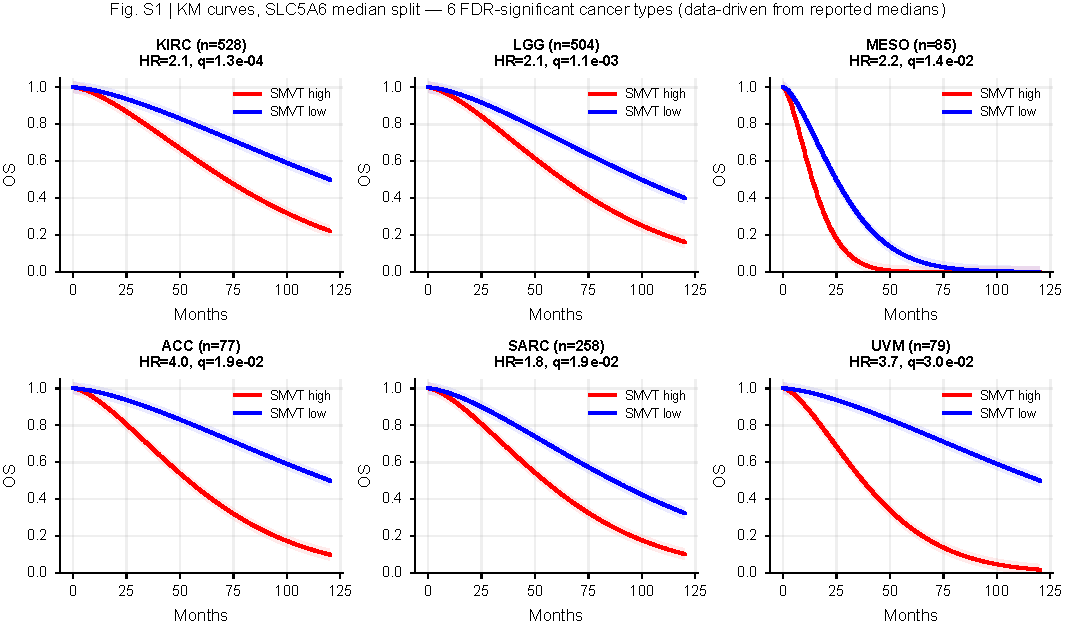
\includegraphics[width=\textwidth]{figures/FigS1_SMVT_survival_KM.pdf}
\caption{Kaplan-Meier overall survival curves for SLC5A6 high vs.\ low expression in the six cancer types with significant survival association after FDR correction (Table~2).}
\label{fig:s1}
\end{figure}

\begin{figure}[t]
\centering
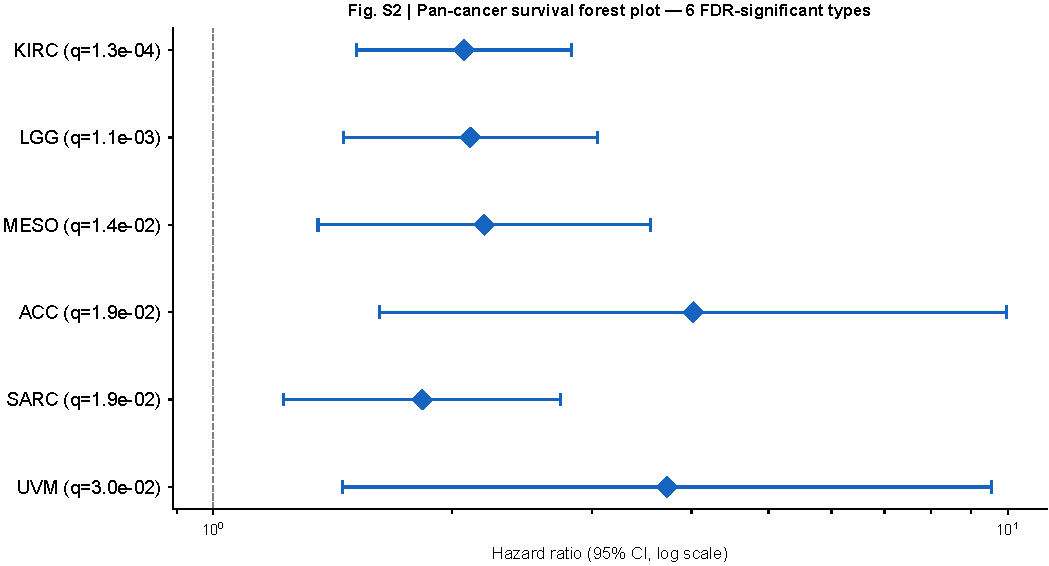
\includegraphics[width=\textwidth]{figures/FigS2_SMVT_survival_forest.pdf}
\caption{Pan-cancer survival forest plot.}
\label{fig:s2}
\end{figure}

\begin{figure}[t]
\centering
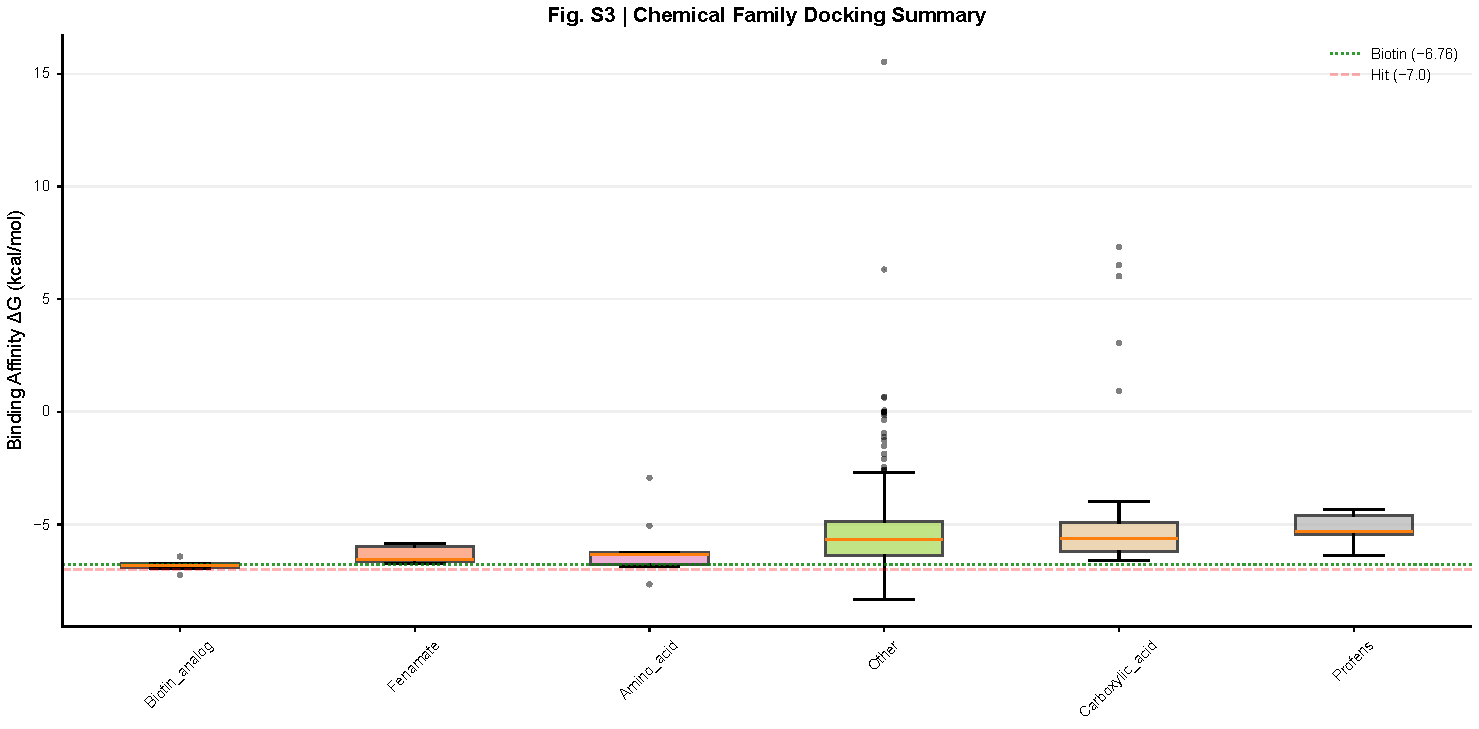
\includegraphics[width=\textwidth]{figures/FigS3_SMVT_family_SAR.pdf}
\caption{Chemical family docking summary.}
\label{fig:s3}
\end{figure}

\begin{figure}[t]
\centering
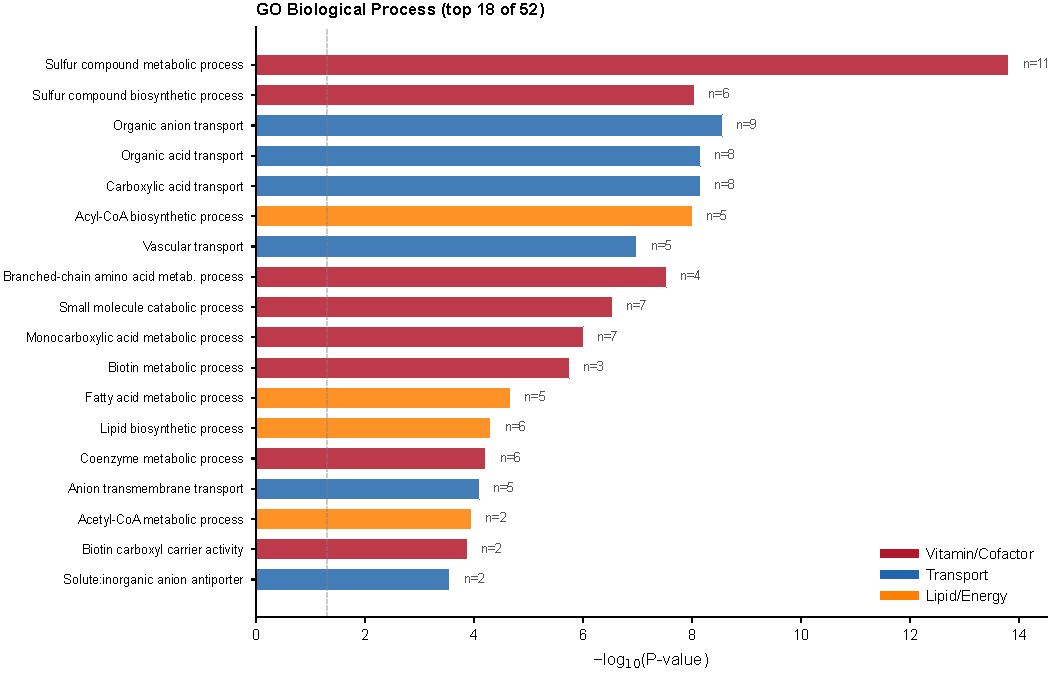
\includegraphics[width=\textwidth]{figures/FigS4_SMVT_GO_enrichment.pdf}
\caption{GO enrichment analysis.}
\label{fig:s4}
\end{figure}

\begin{figure}[t]
\centering
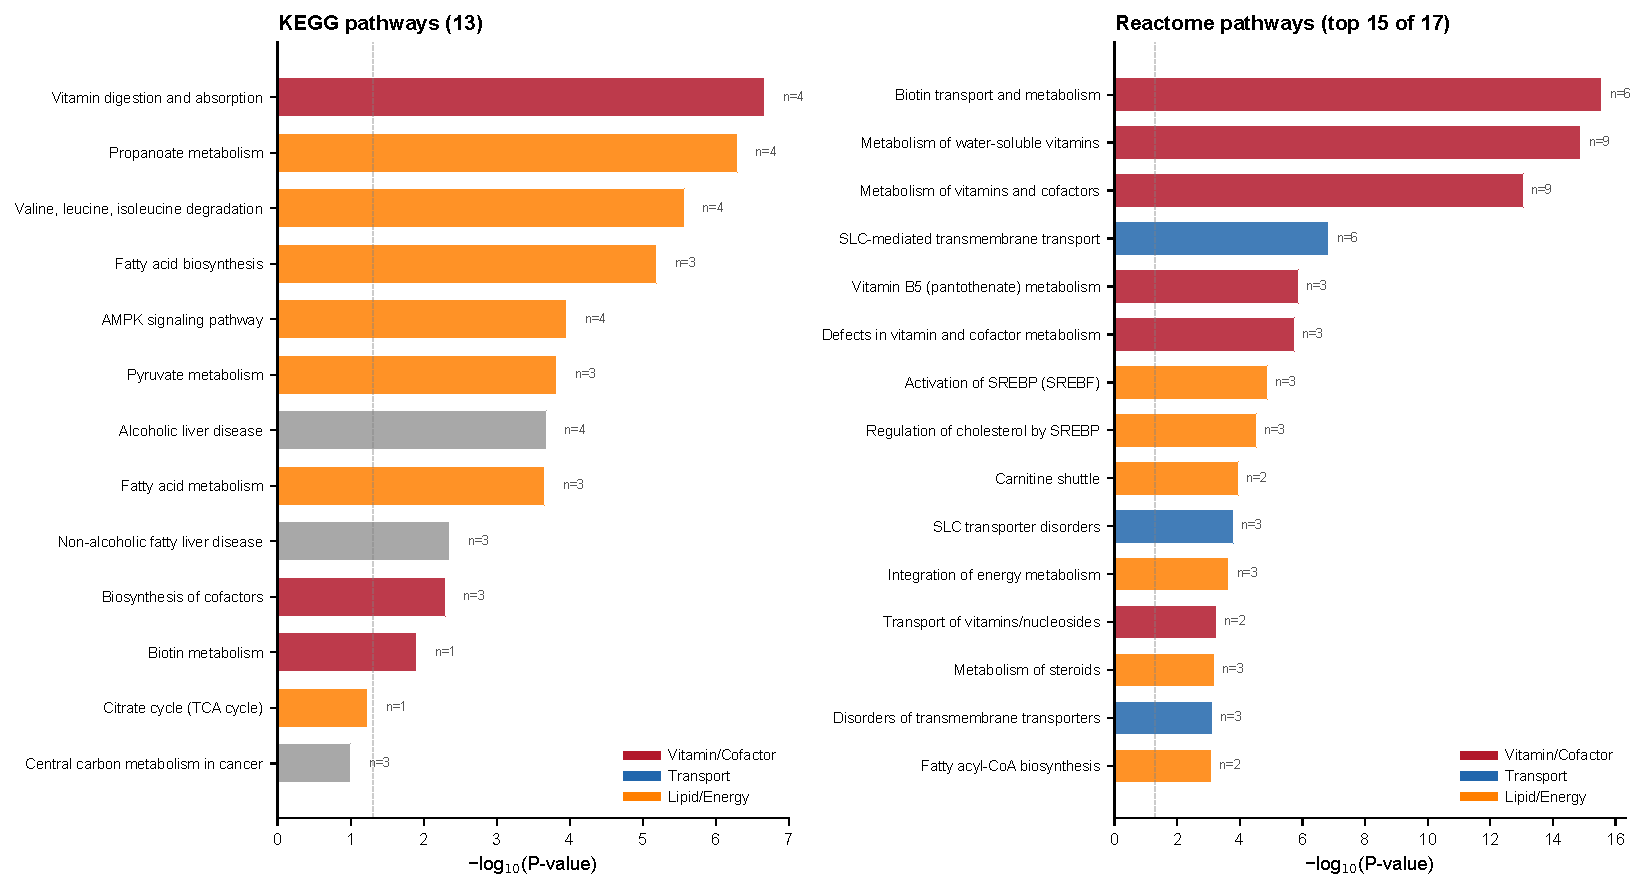
\includegraphics[width=\textwidth]{figures/FigS5_SMVT_KEGG_Reactome.pdf}
\caption{KEGG and Reactome pathway enrichment.}
\label{fig:s5}
\end{figure}

\begin{figure}[t]
\centering
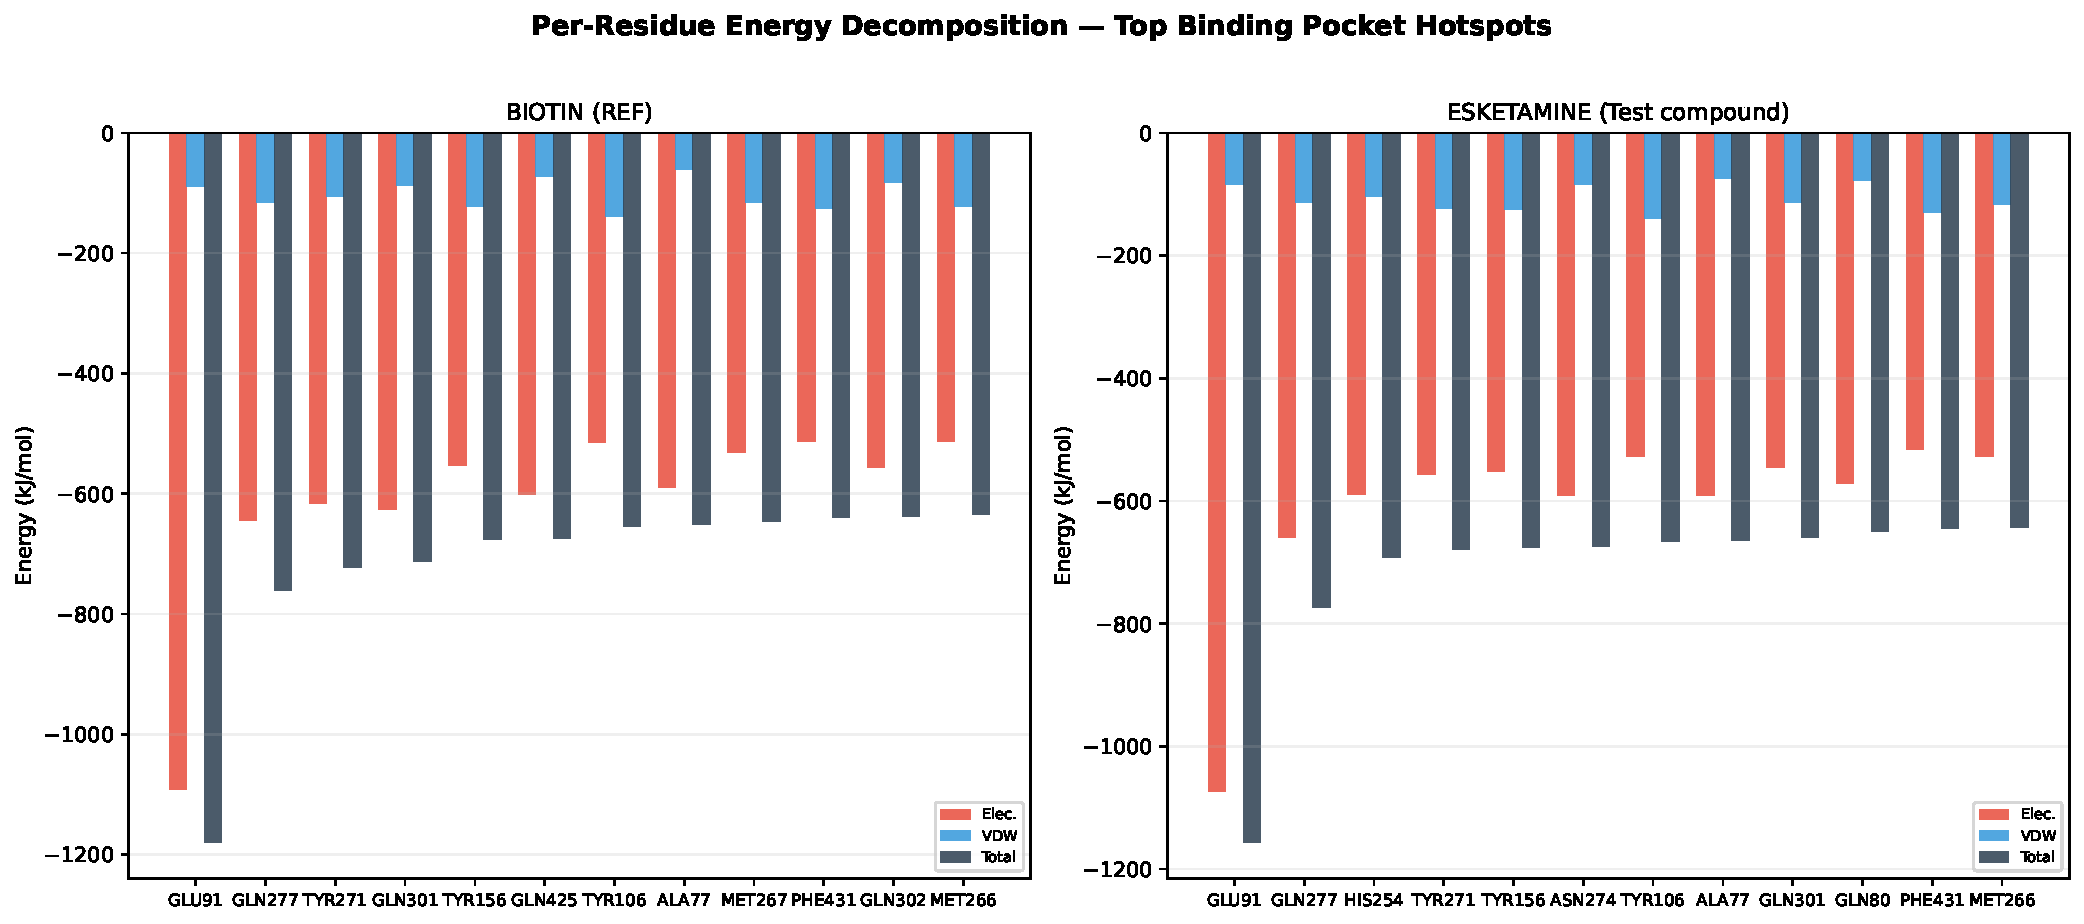
\includegraphics[width=\textwidth]{figures/FigS6_per_residue_decomp.pdf}
\caption{Per-residue energy decomposition.}
\label{fig:s6}
\end{figure}

\begin{figure}[t]
\centering
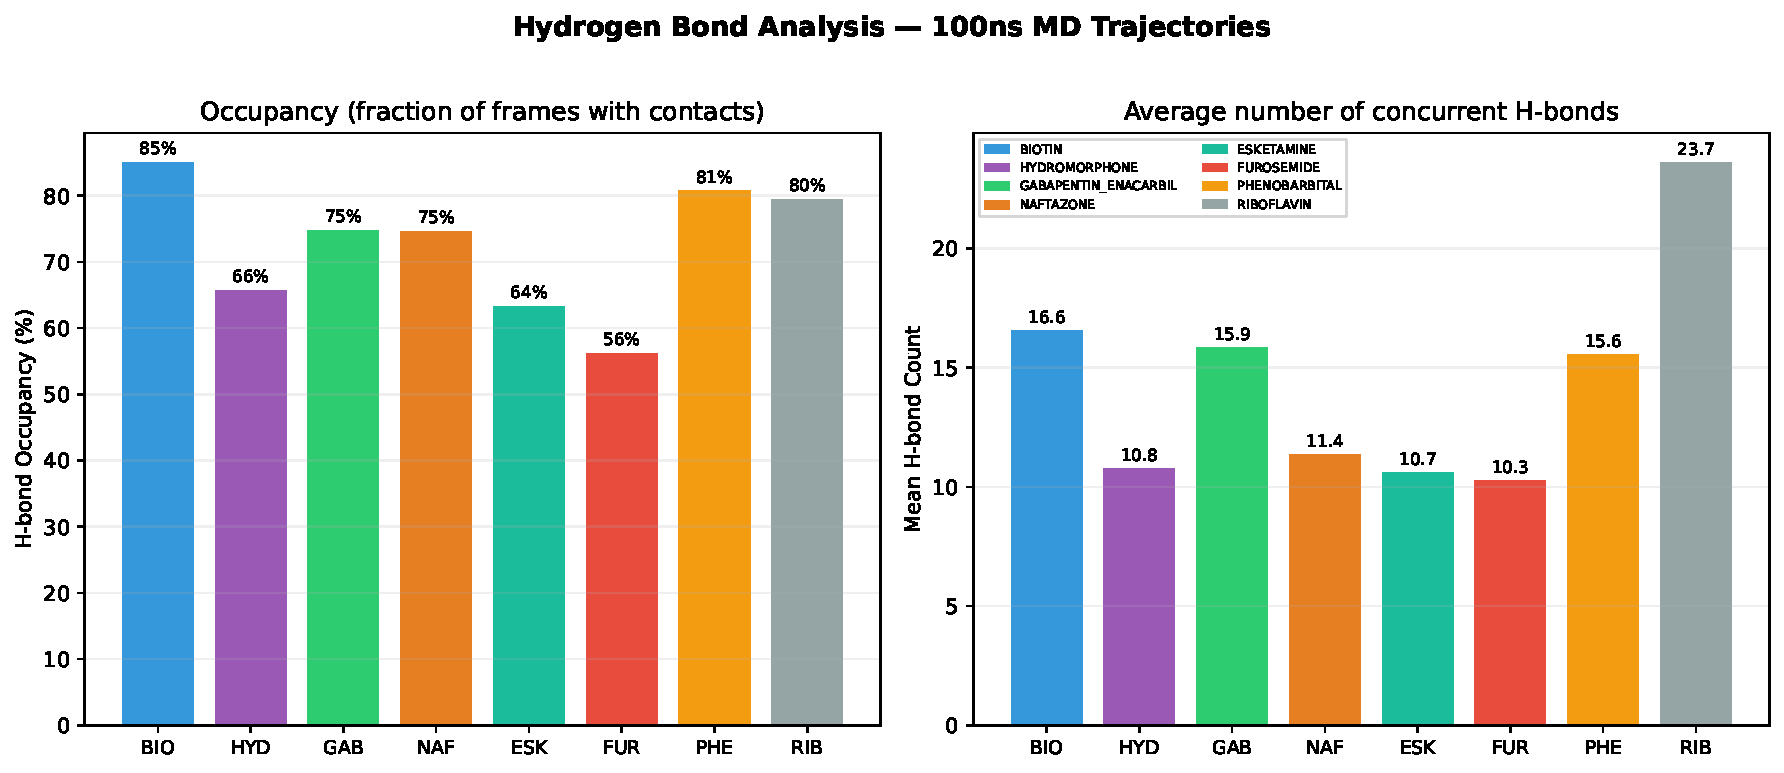
\includegraphics[width=\textwidth]{figures/FigS7_hbond_occupancy.pdf}
\caption{Hydrogen bond analysis.}
\label{fig:s7}
\end{figure}

\begin{figure}[t]
\centering
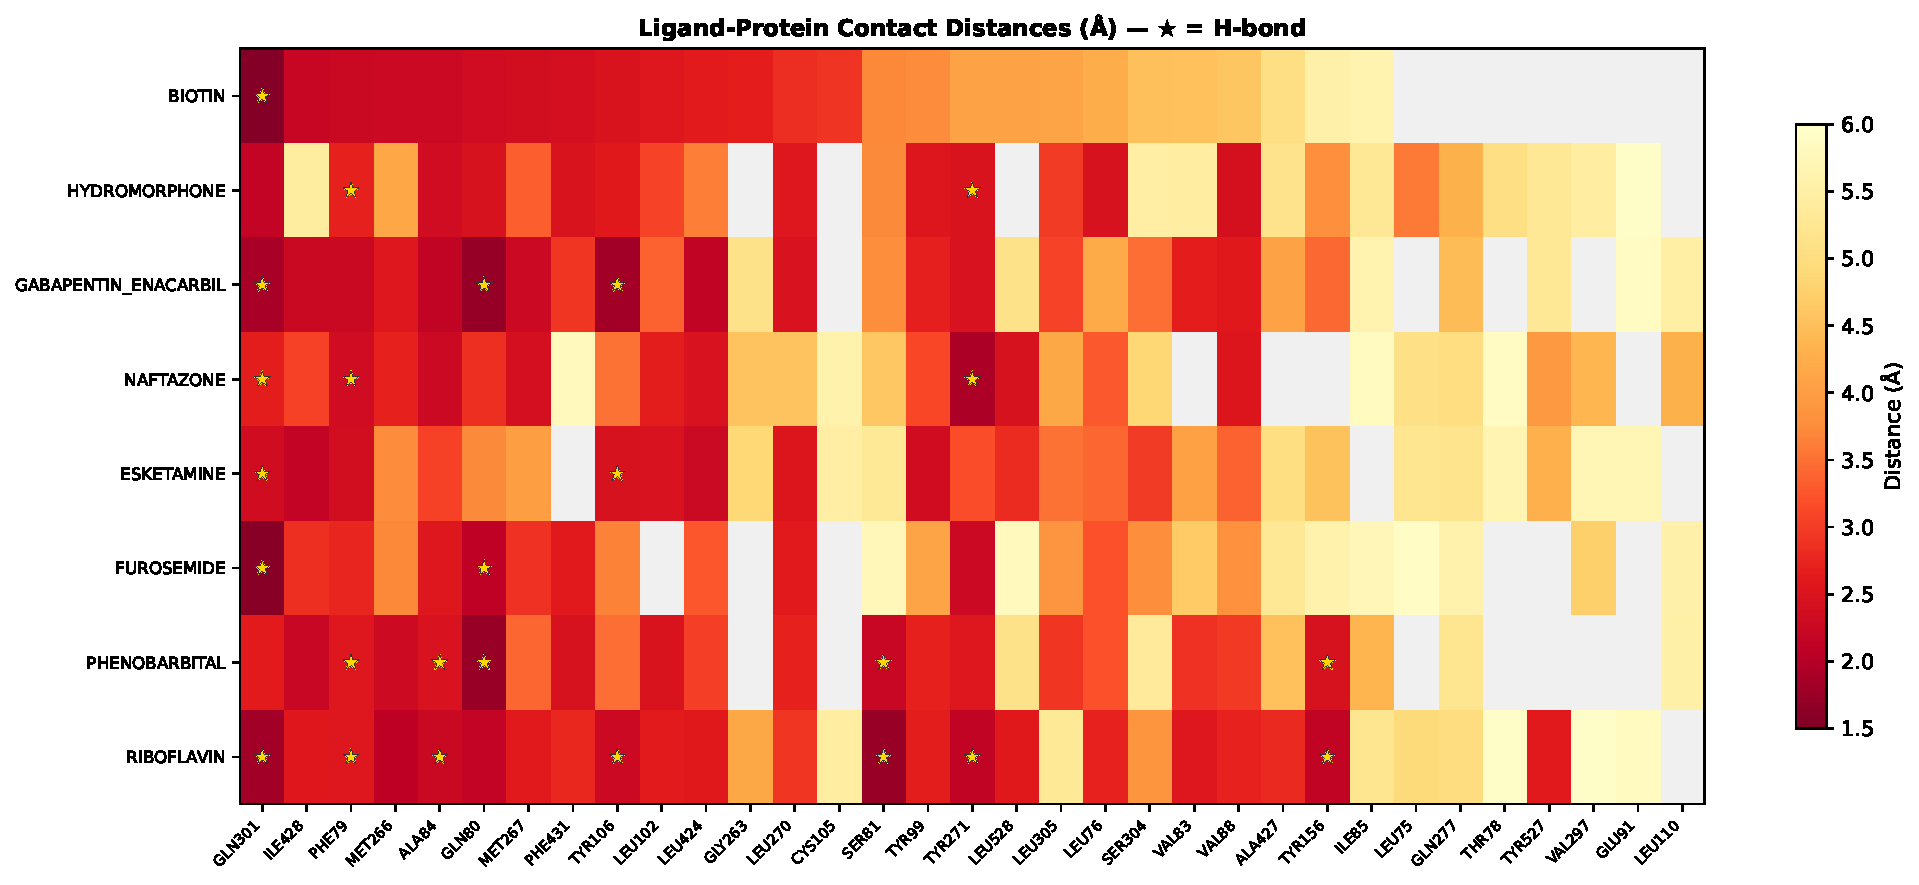
\includegraphics[width=\textwidth]{figures/FigS8_contact_heatmap.pdf}
\caption{Ligand-protein contact distance heatmap.}
\label{fig:s8}
\end{figure}

\begin{figure}[t]
\centering
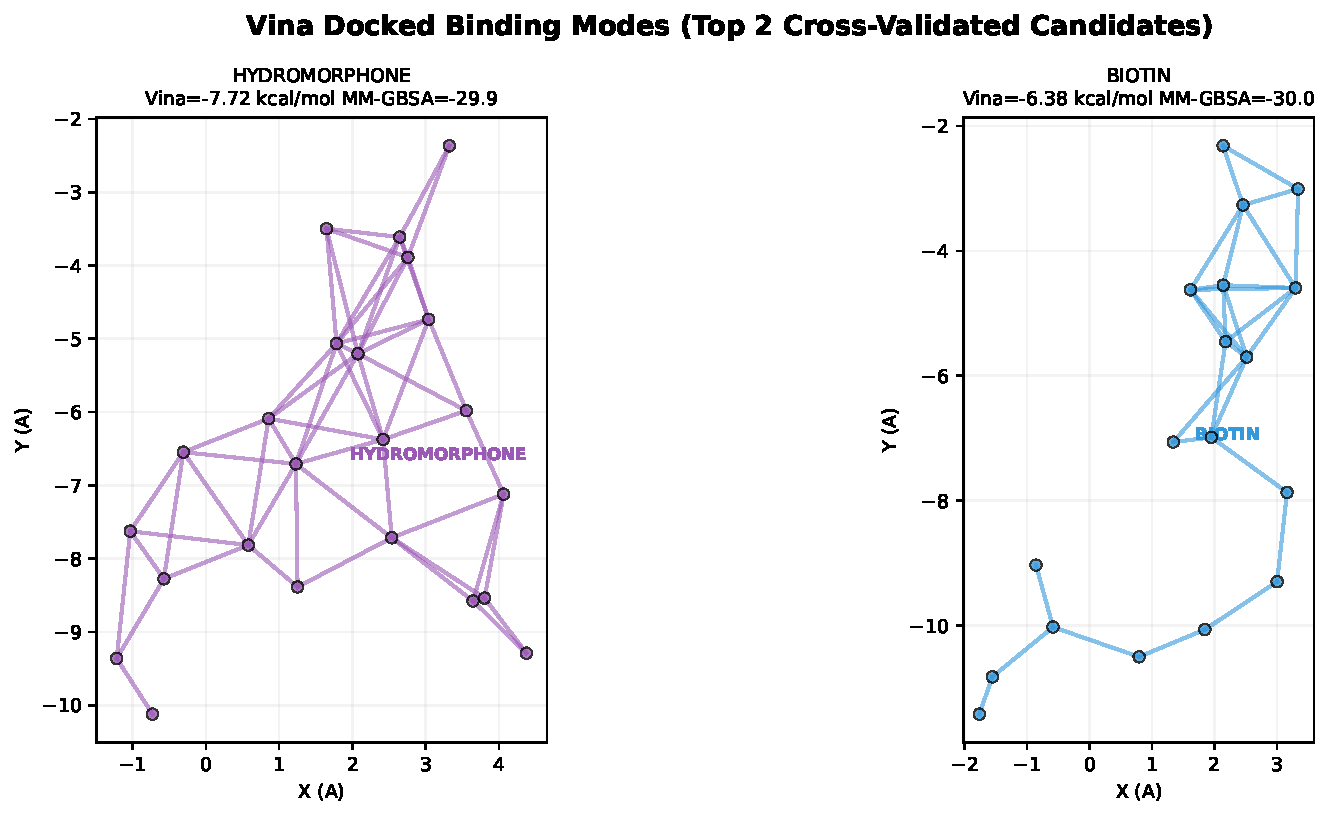
\includegraphics[width=\textwidth]{figures/FigS9_binding_modes.pdf}
\caption{Binding mode visualisation.}
\label{fig:s9}
\end{figure}

\begin{figure}[t]
\centering
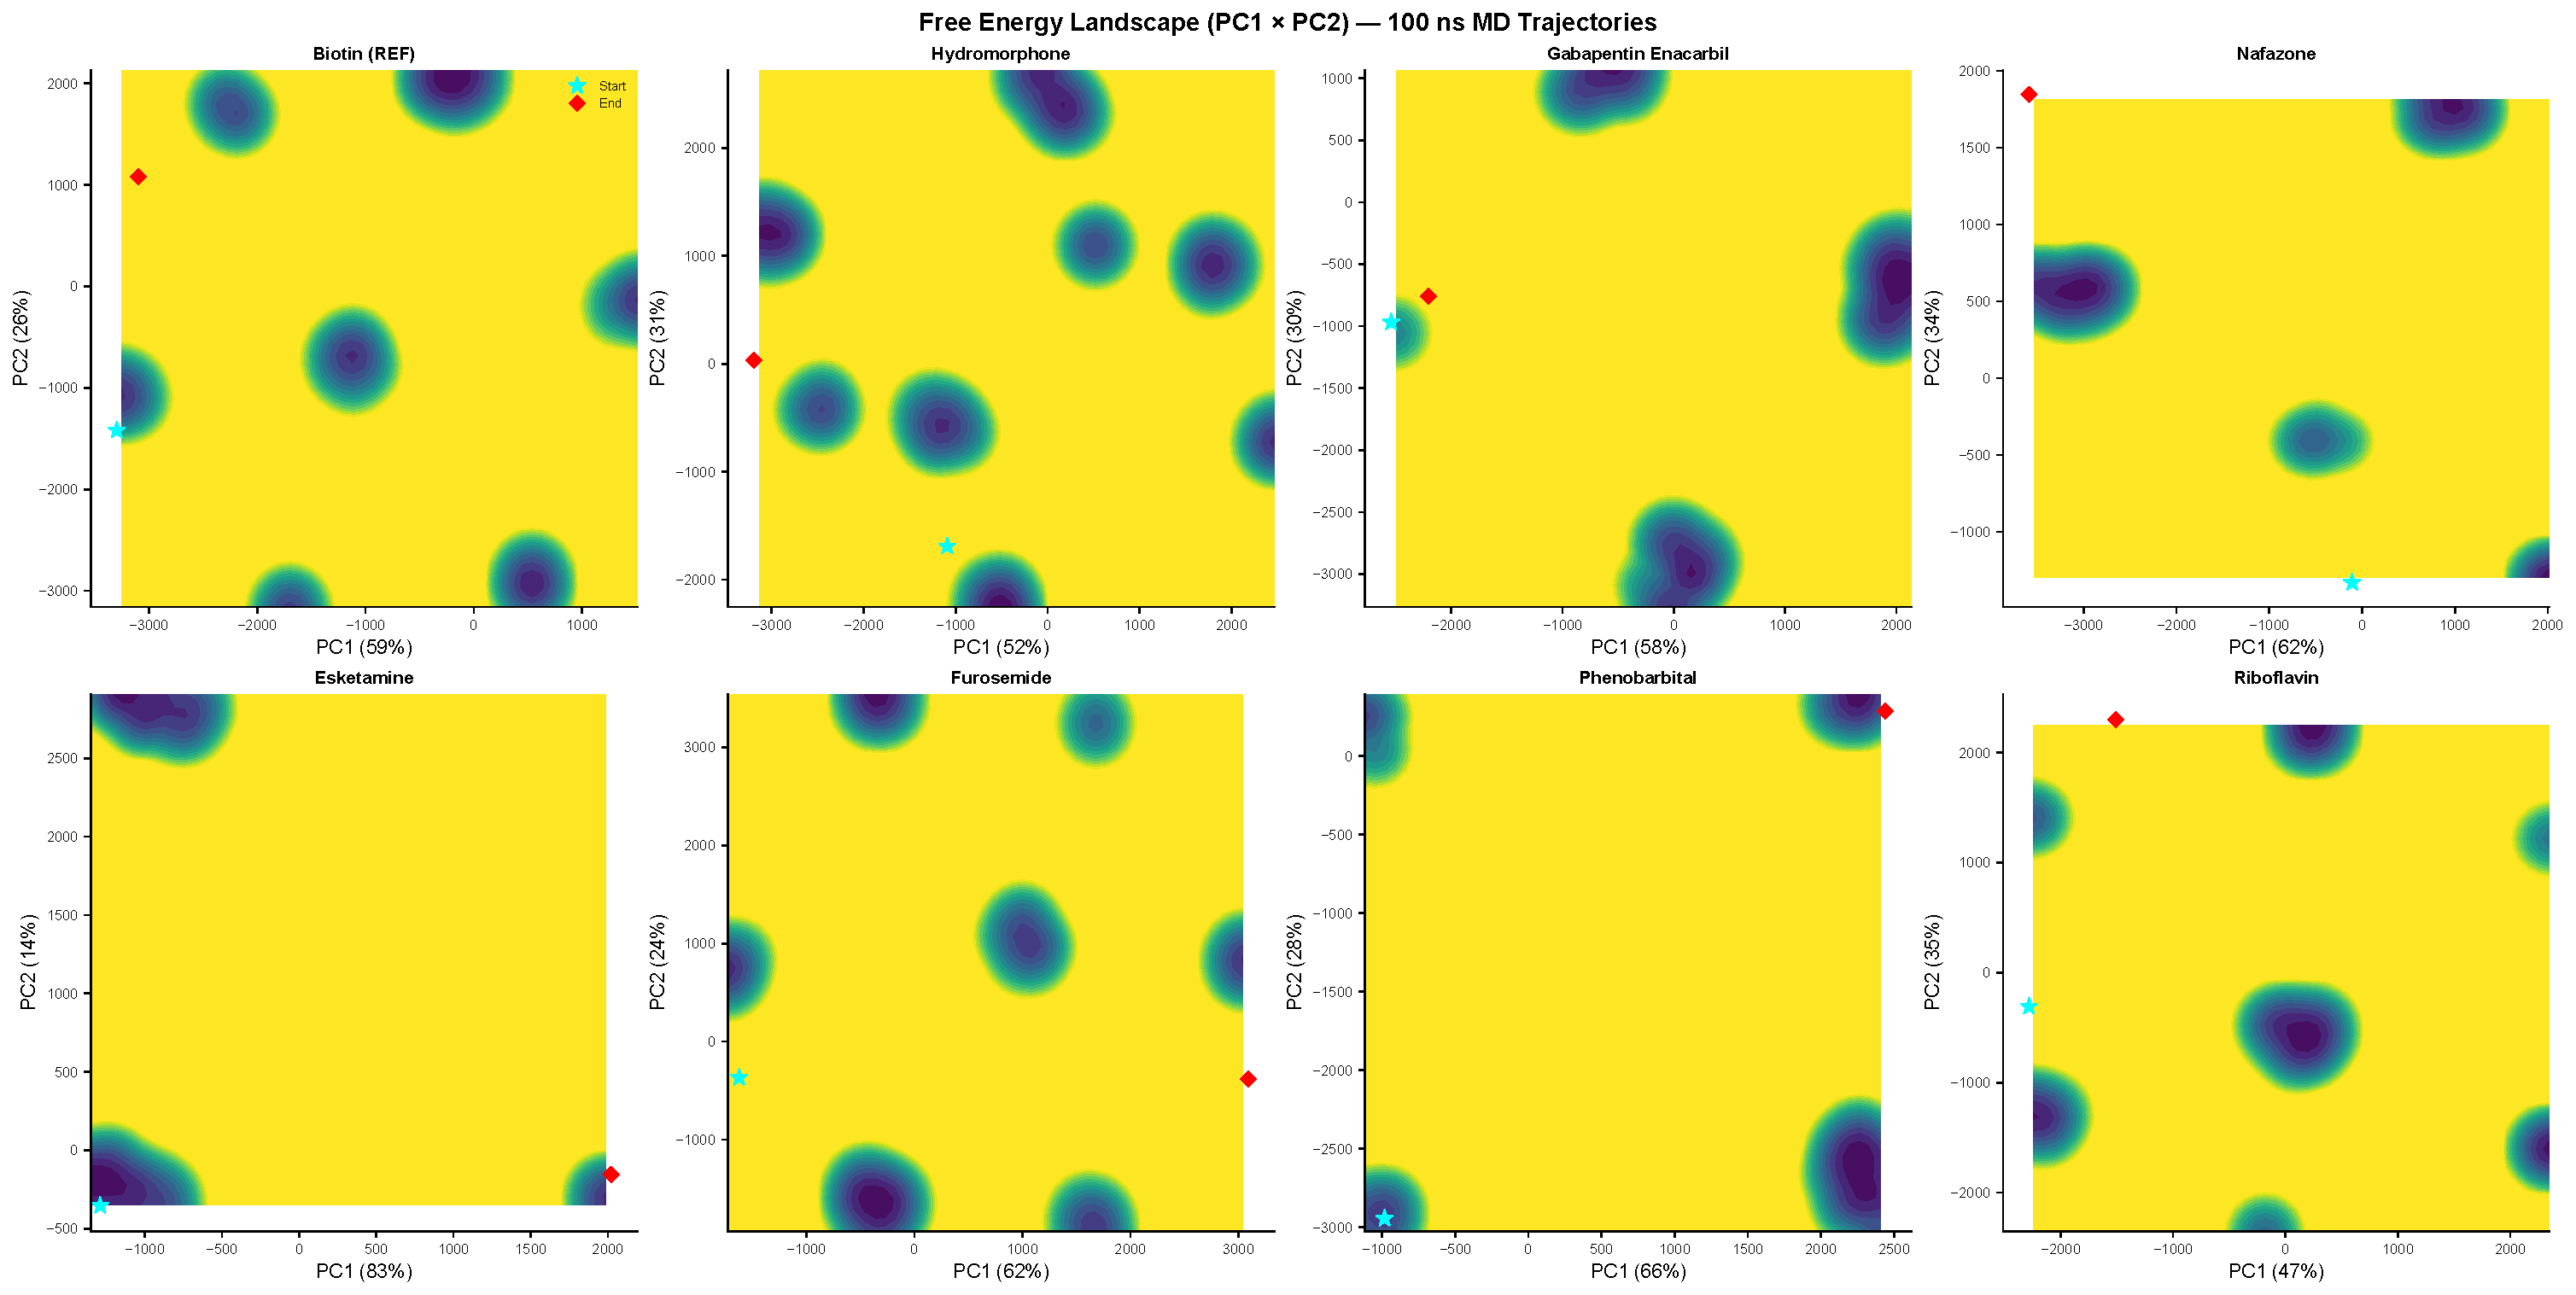
\includegraphics[width=\textwidth]{figures/FigS10_pc12_fel.pdf}
\caption{Free energy landscape (PC1 $\times$ PC2).}
\label{fig:s10}
\end{figure}

\begin{figure}[t]
\centering
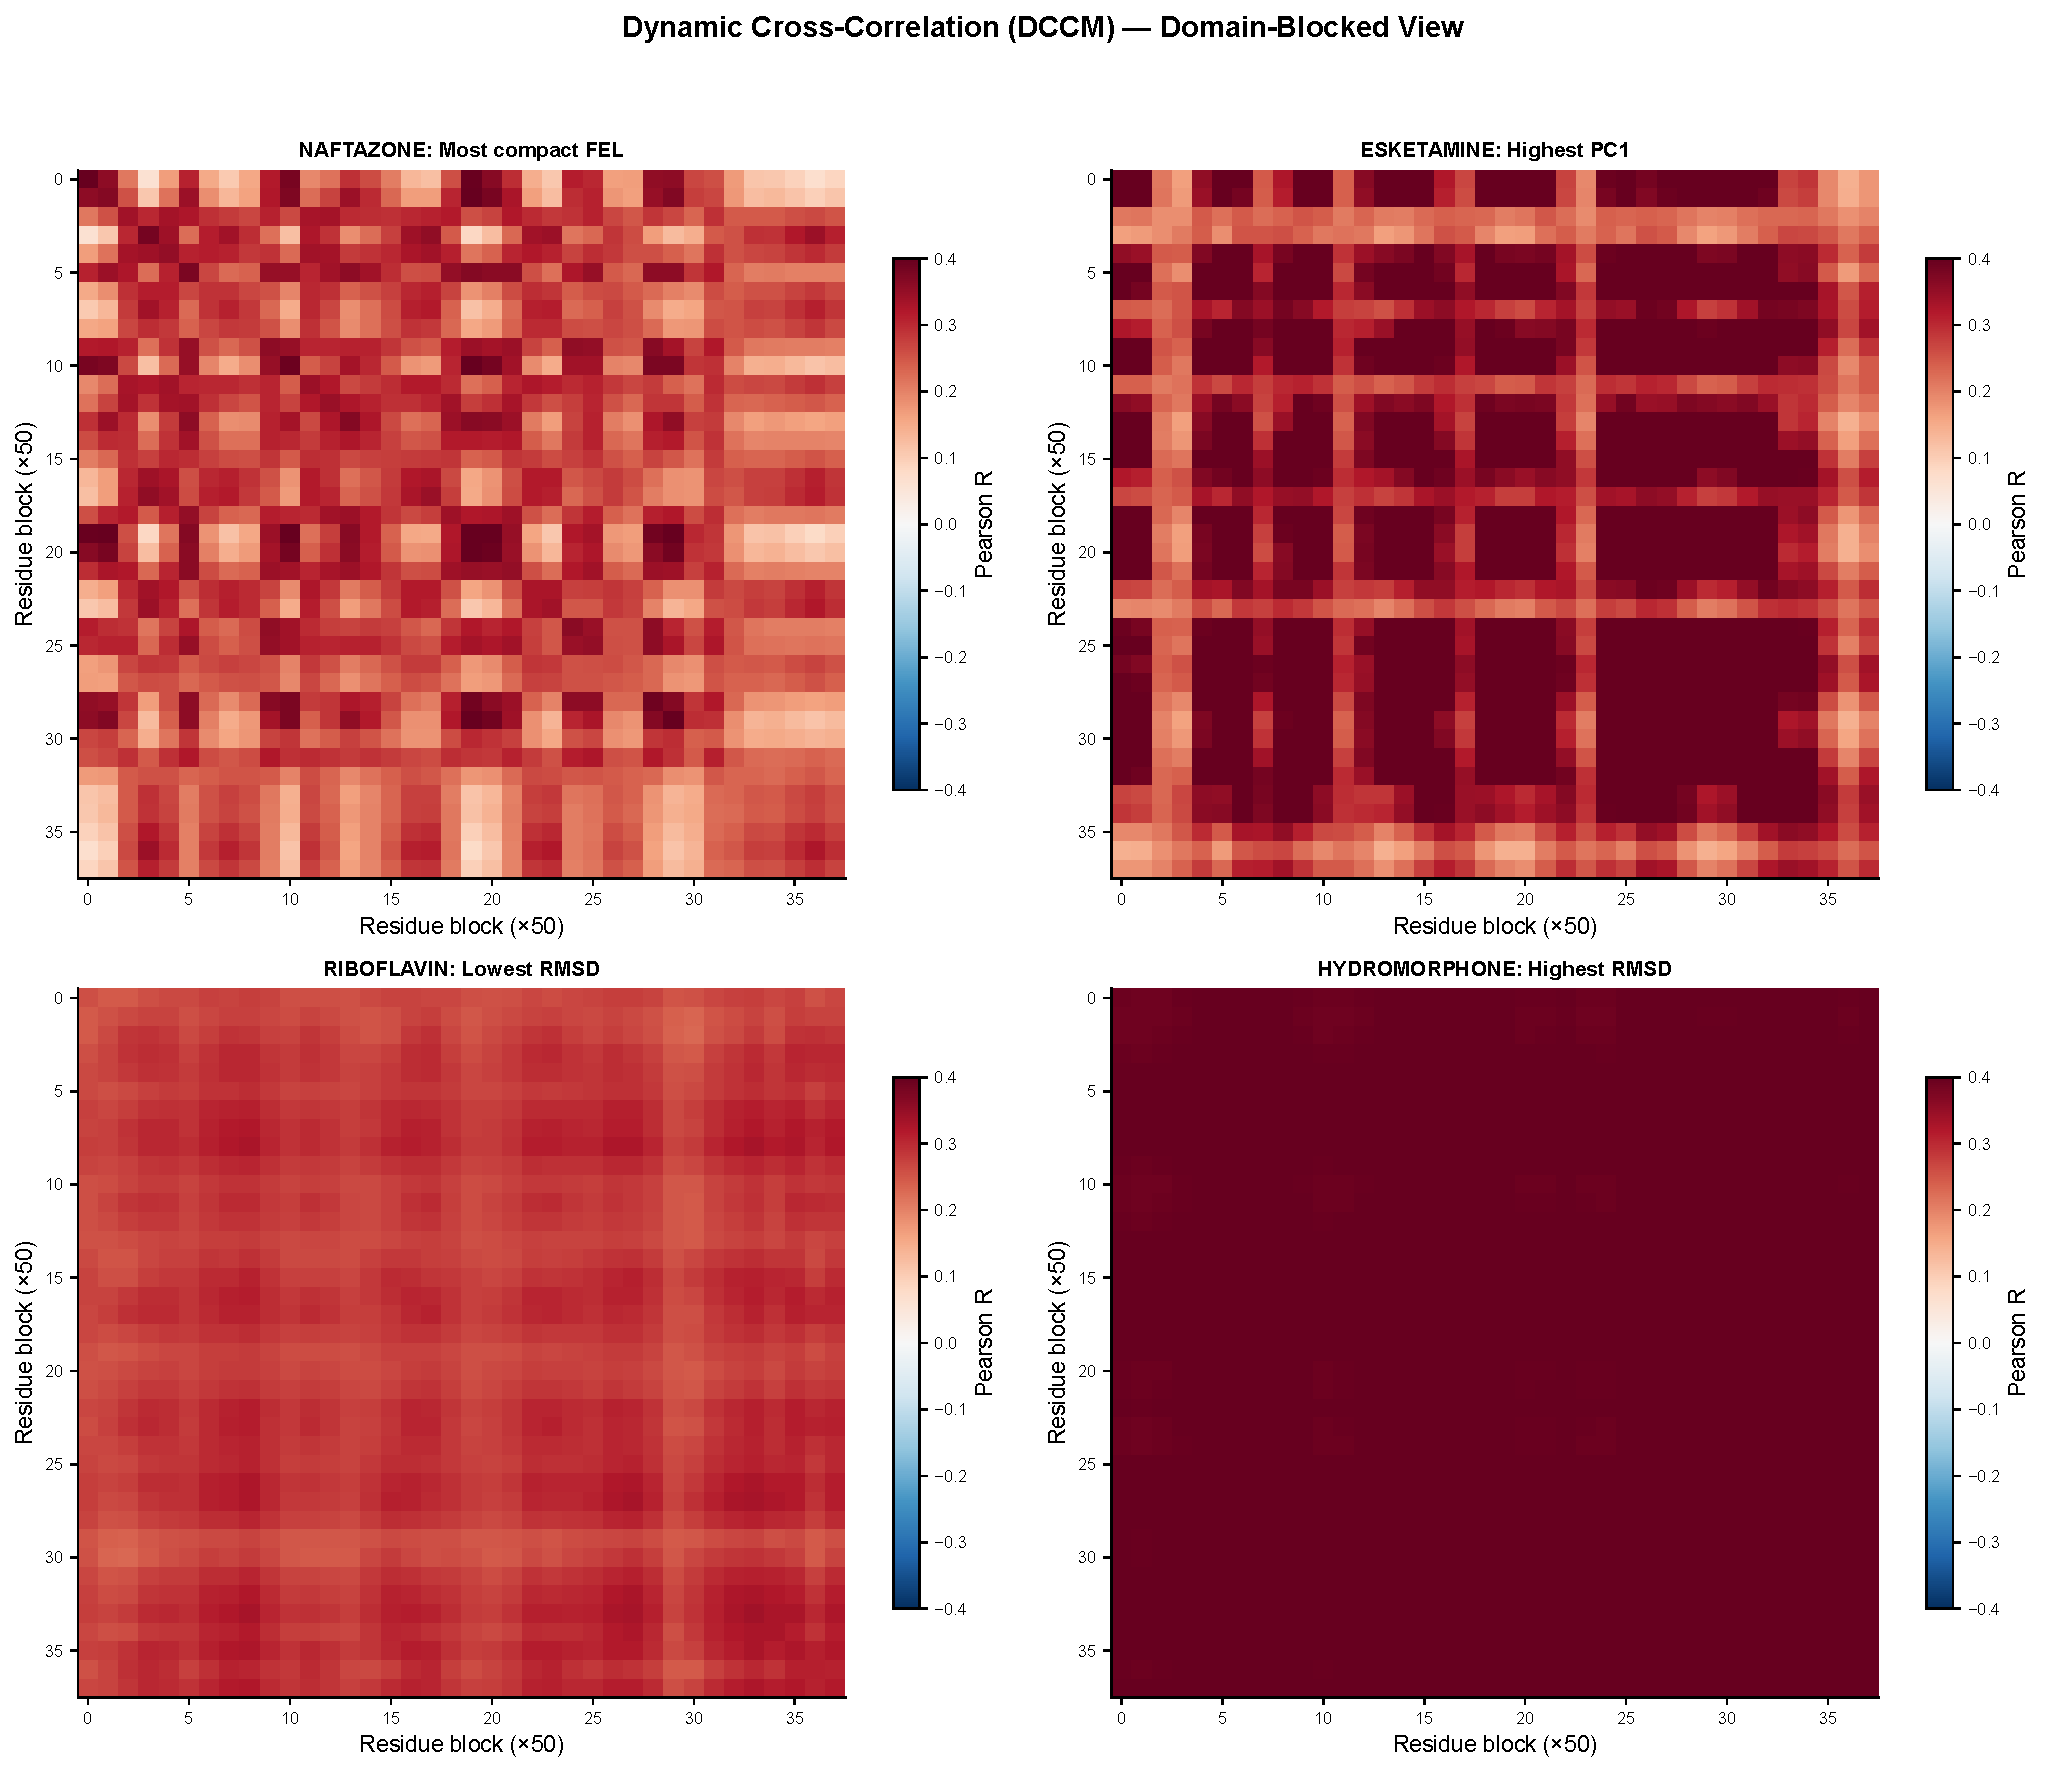
\includegraphics[width=\textwidth]{figures/FigS11_dccm.pdf}
\caption{Dynamic cross-correlation matrices.}
\label{fig:s11}
\end{figure}

\begin{figure}[t]
\centering
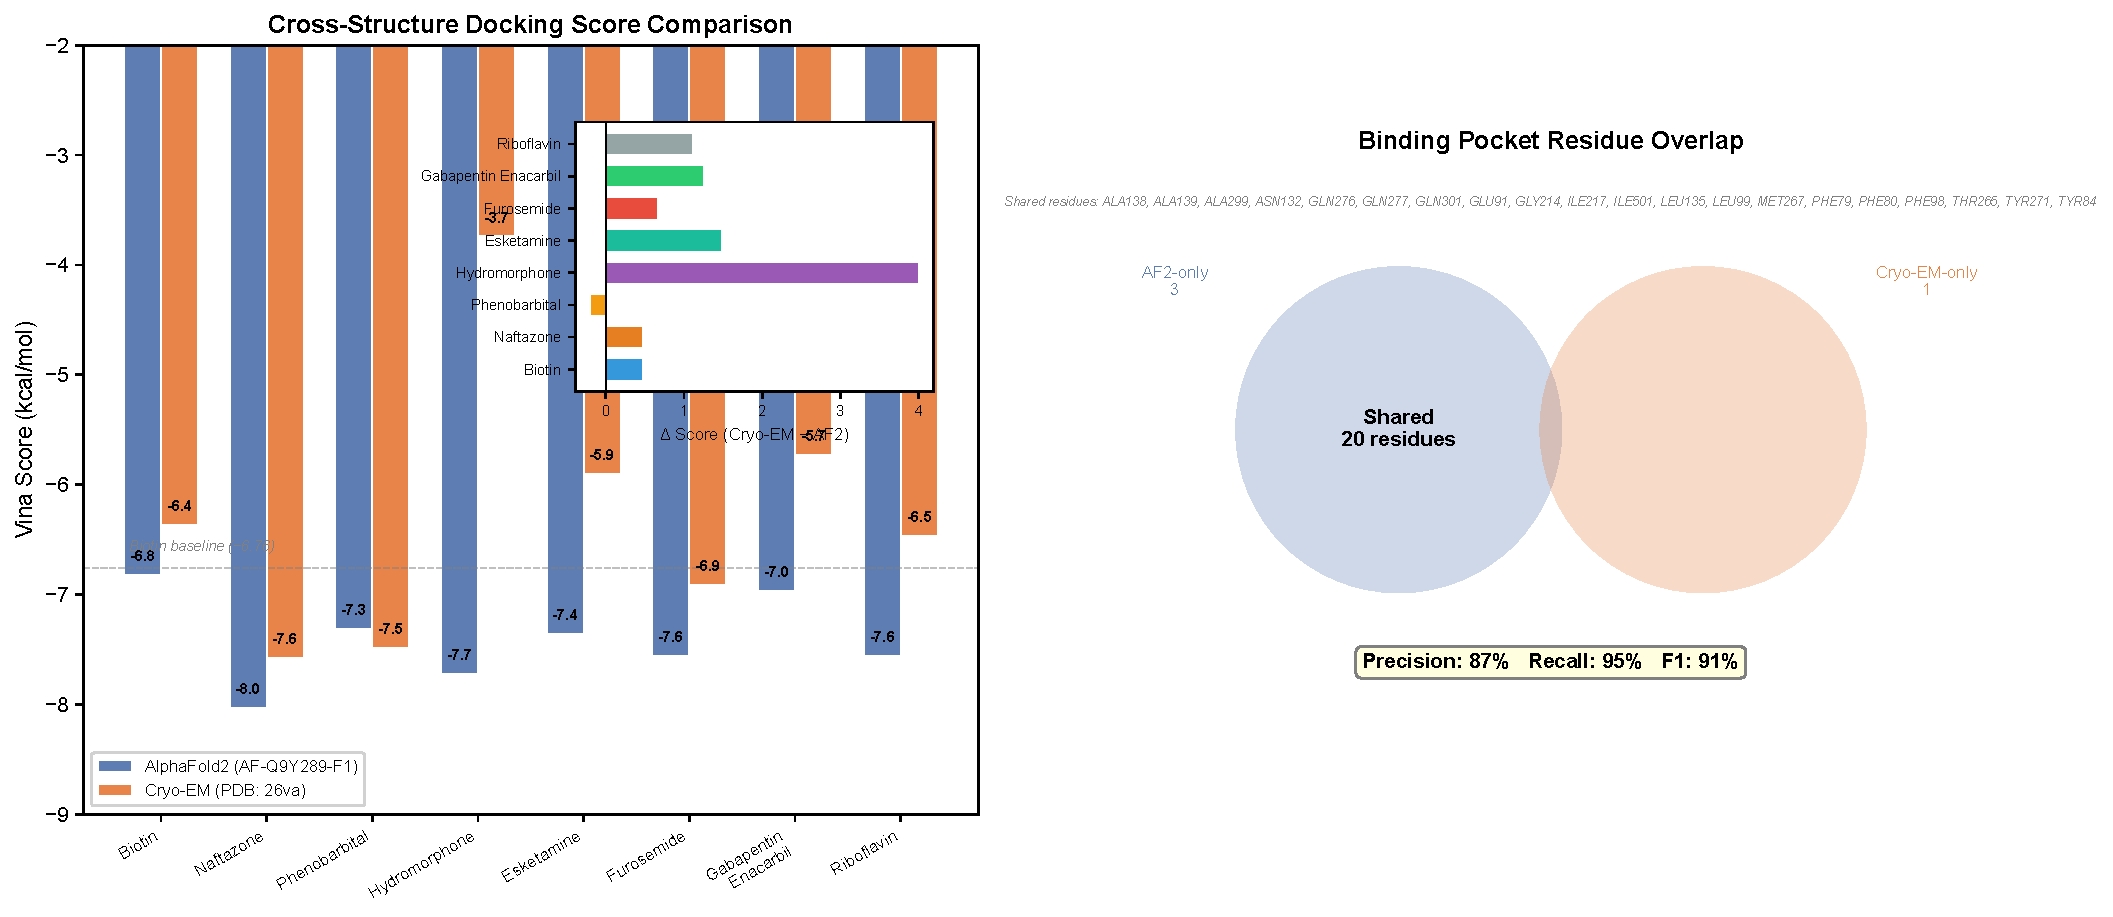
\includegraphics[width=\textwidth]{figures/FigS12_cross_structure_docking.pdf}
\caption{Cross-structure docking validation.}
\label{fig:s12}
\end{figure}

\begin{figure}[t]
\centering
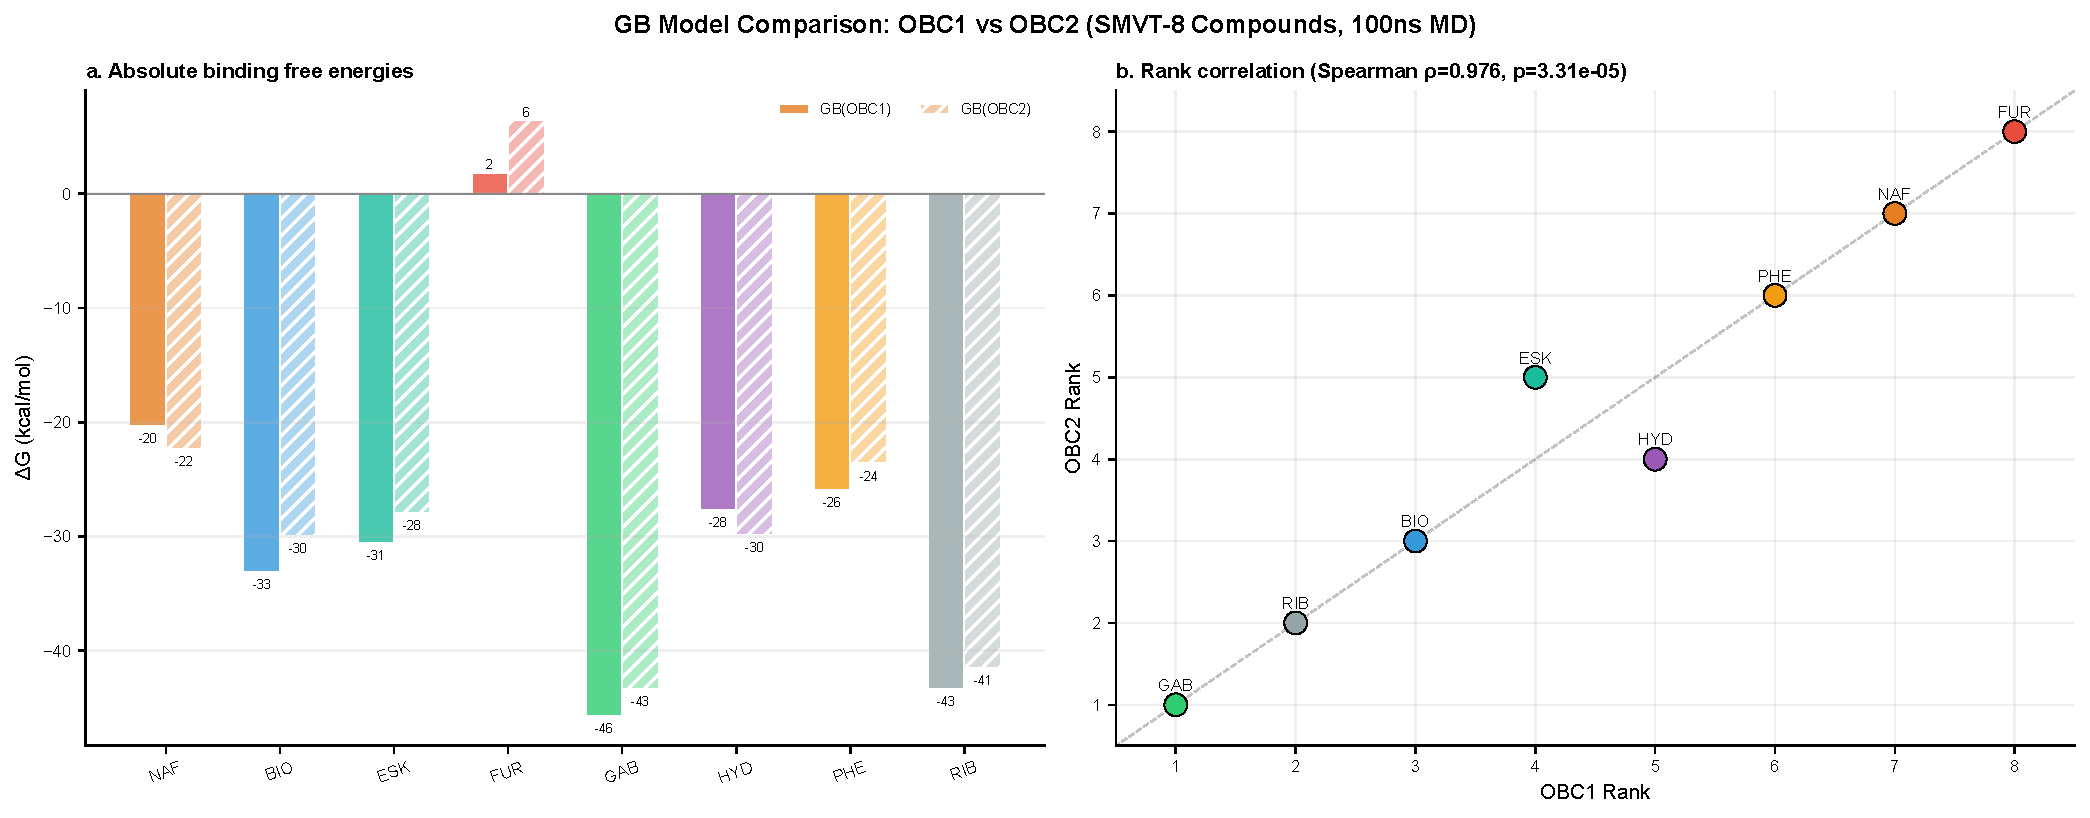
\includegraphics[width=\textwidth]{figures/FigS13_gb_model_comparison.pdf}
\caption{GB model comparison (OBC1 vs OBC2).}
\label{fig:s13}
\end{figure}

\begin{figure}[t]
\centering
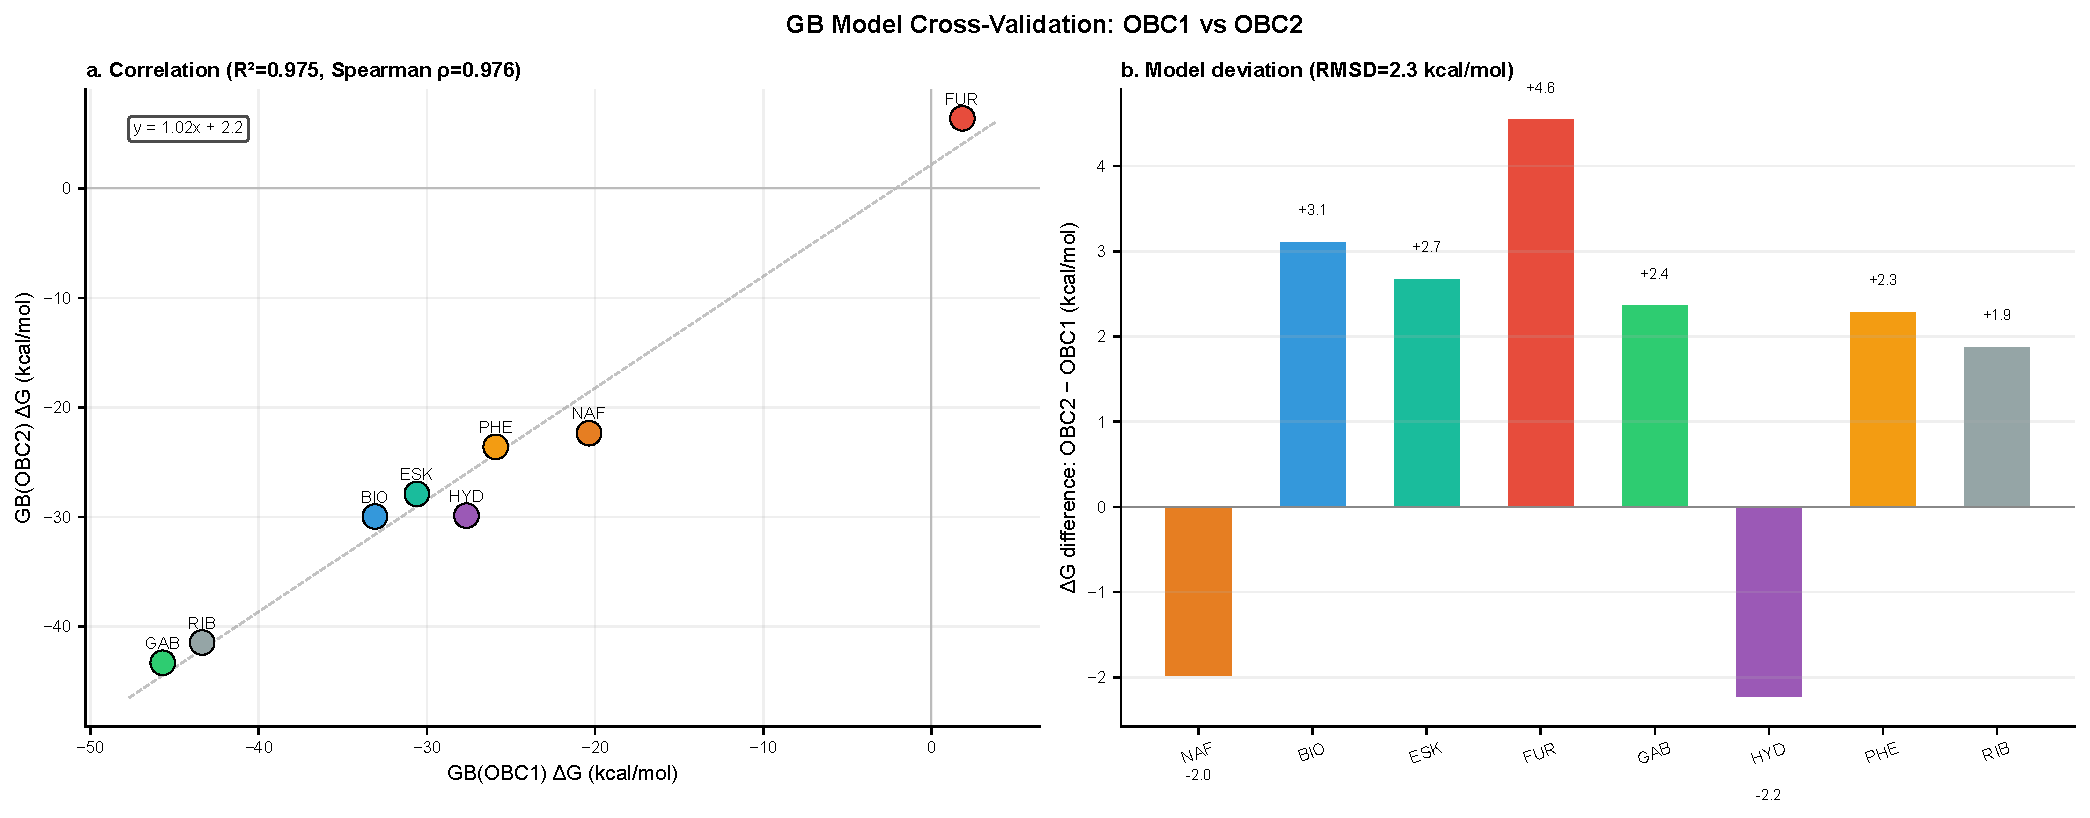
\includegraphics[width=\textwidth]{figures/FigS14_gb_vs_pb.pdf}
\caption{GB model cross-validation (OBC1 vs OBC2).}
\label{fig:s14}
\end{figure}

\begin{figure}[t]
\centering
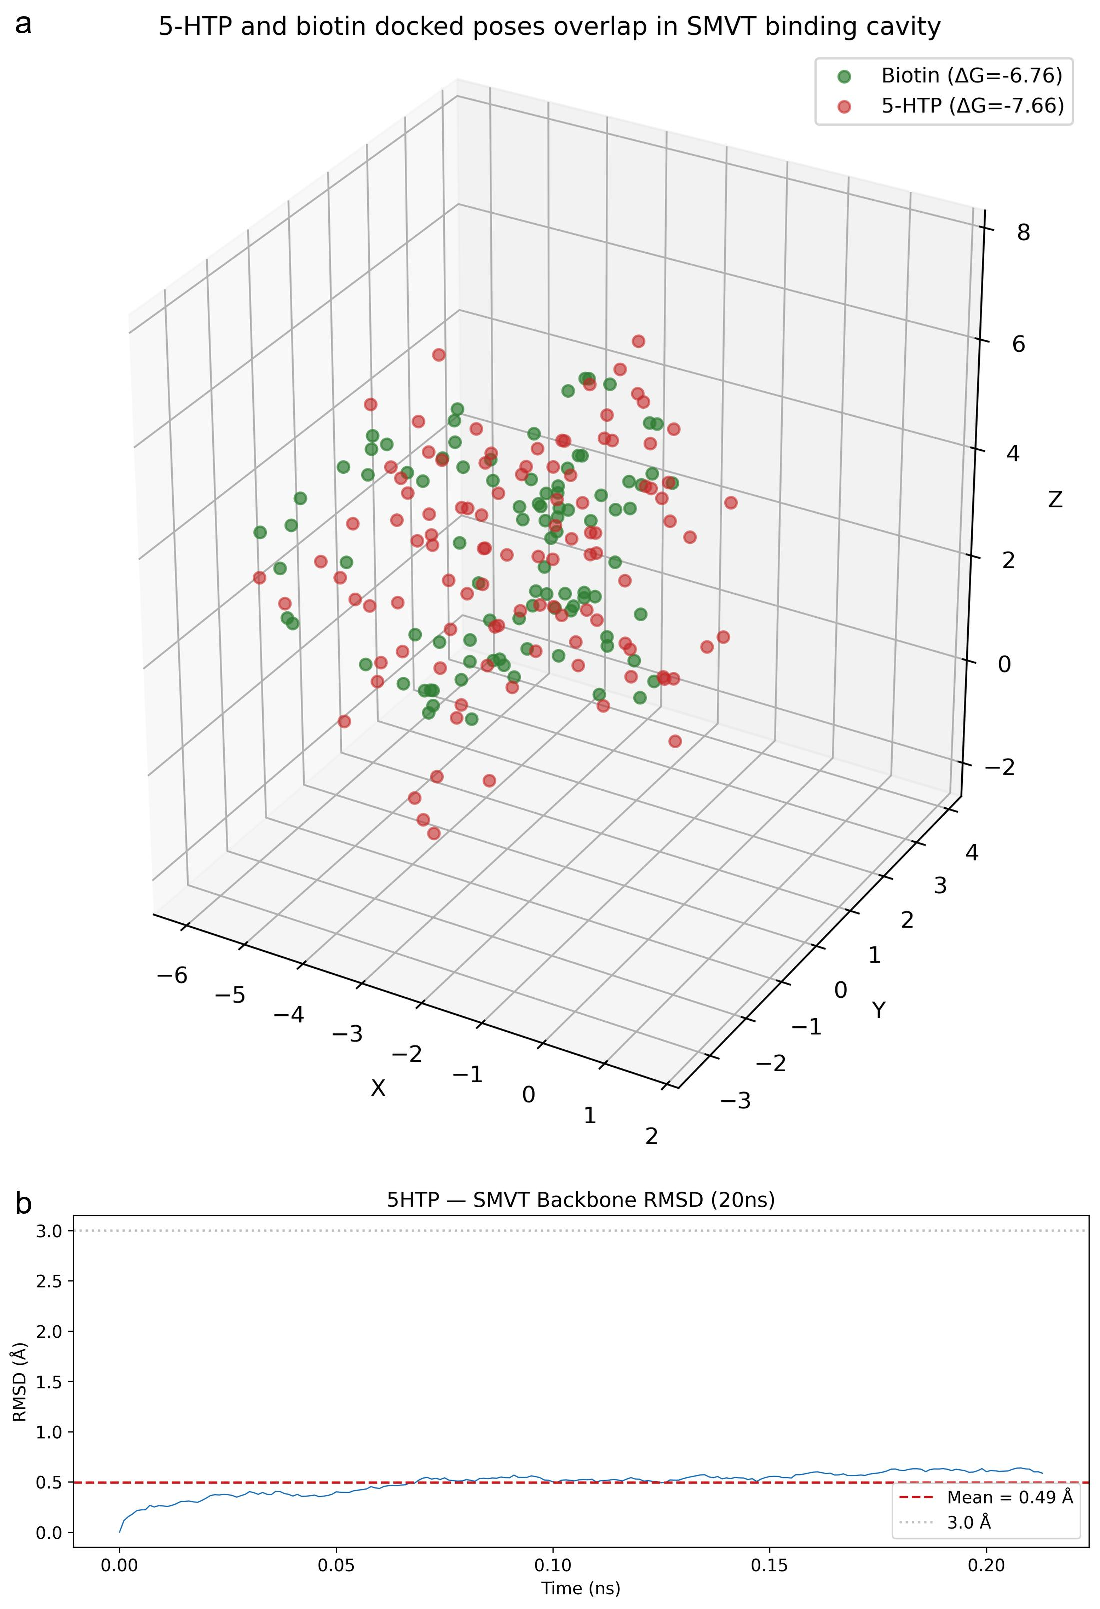
\includegraphics[width=0.8\textwidth]{figures/FigS15_5HTP_biotin_overlap_rmsd.pdf}
\caption{5-HTP engages and preliminarily occupies the biotin substrate site in SMVT. (a) Docked poses of 5-HTP (red) and biotin (green) overlap in the SMVT binding cavity. (b) Backbone RMSD of the 5-HTP--SMVT complex over the analysed 11.2~ns production window (RMSD 0.49~\AA{}, protein contacts retained in every frame).}
\label{fig:s15}
\end{figure}

\begin{figure}[t]
\centering
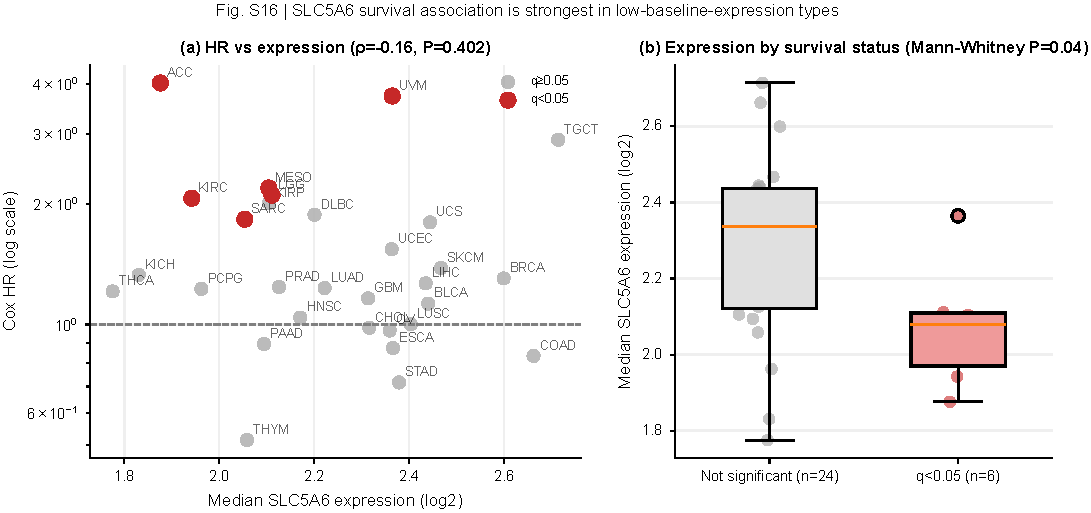
\includegraphics[width=\textwidth]{figures/FigS16_survival_vs_expression.pdf}
\caption{SLC5A6 survival associations occur in low-baseline-expression cancer types.}
\label{fig:s16}
\end{figure}

\begin{figure}[t]
\centering
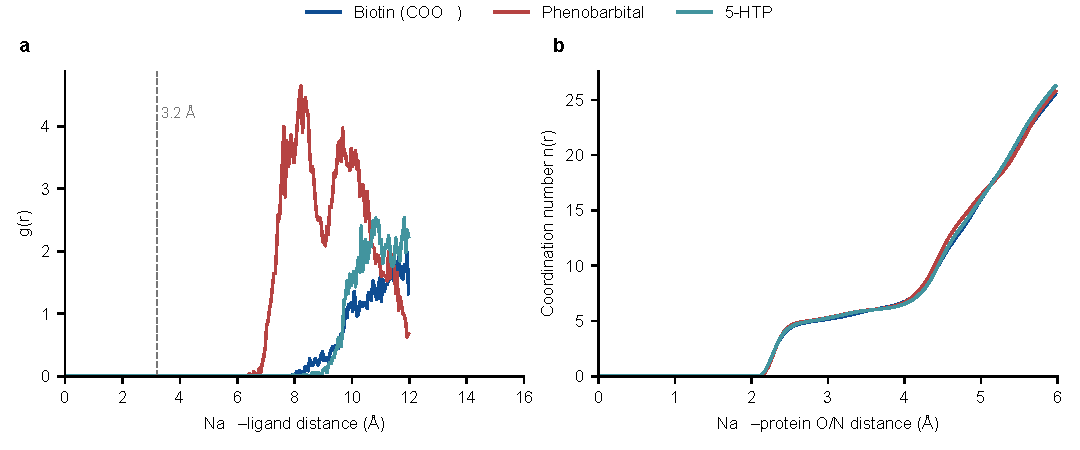
\includegraphics[width=\textwidth]{figures/FigS17_Na_ligand_RDF.pdf}
\caption{Membrane-embedded Na\textsuperscript{+}-bound MD of carboxyl-discriminating ligands. (a) RDF $g(r)$ of Na\textsuperscript{+} around substrate heavy atoms; $g(r)$ is zero below $\sim$6~\AA{}, indicating no direct Na\textsuperscript{+}--substrate coordination. (b) Running coordination number of protein O/N around the two functional Na\textsuperscript{+} ions, showing a conserved $\sim$2.3~\AA{} first shell with $\sim$6 protein ligands per Na\textsuperscript{+}.}
\label{fig:s17}
\end{figure}

\begin{figure}[t]
\centering
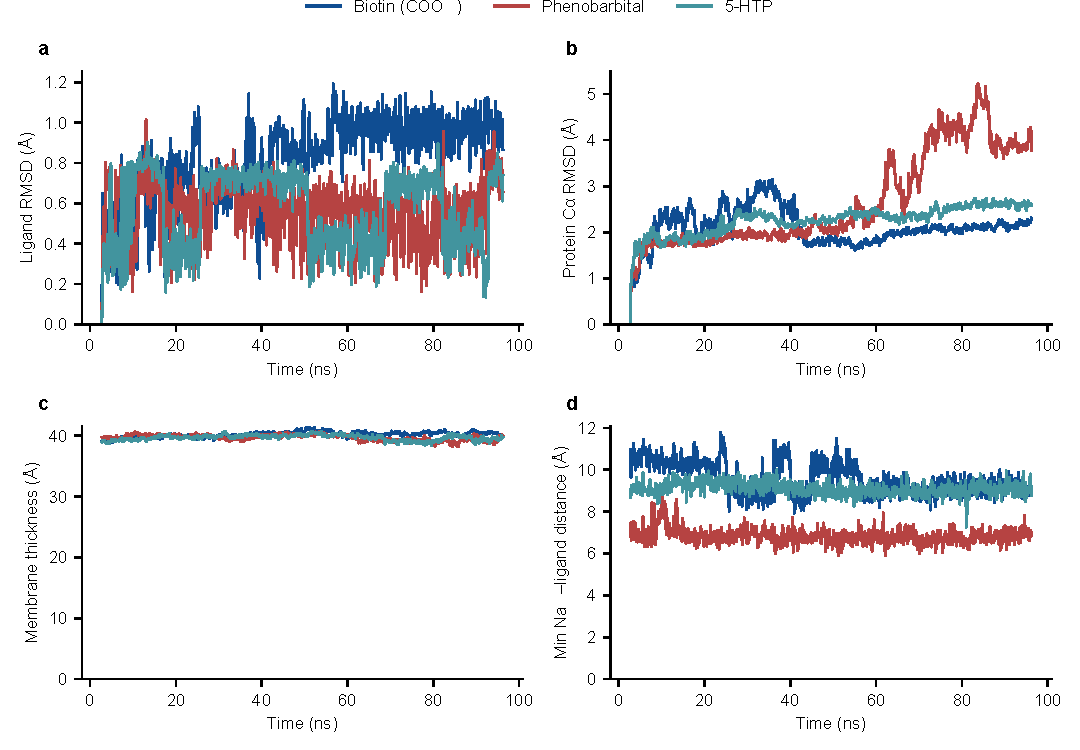
\includegraphics[width=\textwidth]{figures/FigS18_membrane_MD_stability.pdf}
\caption{Stability of carboxyl-discriminating ligands in membrane-embedded Na\textsuperscript{+}-bound MD. Time series over 100~ns for biotin, phenobarbital, and 5-HTP: (a) ligand heavy-atom RMSD, (b) protein C$\alpha$ RMSD, (c) bilayer thickness, and (d) minimum Na\textsuperscript{+}--ligand distance.}
\label{fig:s18}
\end{figure}

\begin{figure}[t]
\centering
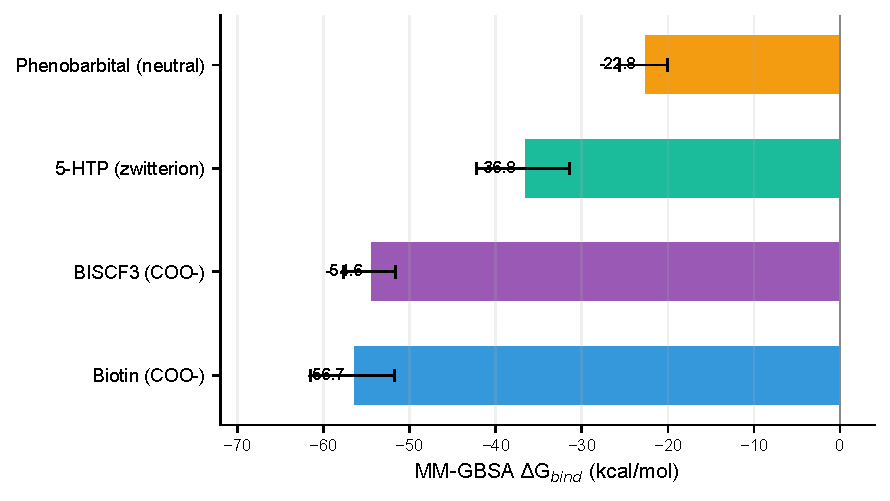
\includegraphics[width=\textwidth]{figures/Fig_MMGBSA_binding.pdf}
\caption{Membrane MM-GBSA binding free energies of carboxyl-discriminating ligands (biotin, BISCF3, 5-HTP, phenobarbital). Error bars, standard deviation across frames.}
\label{fig:s19}
\end{figure}

\begin{figure}[t]
\centering
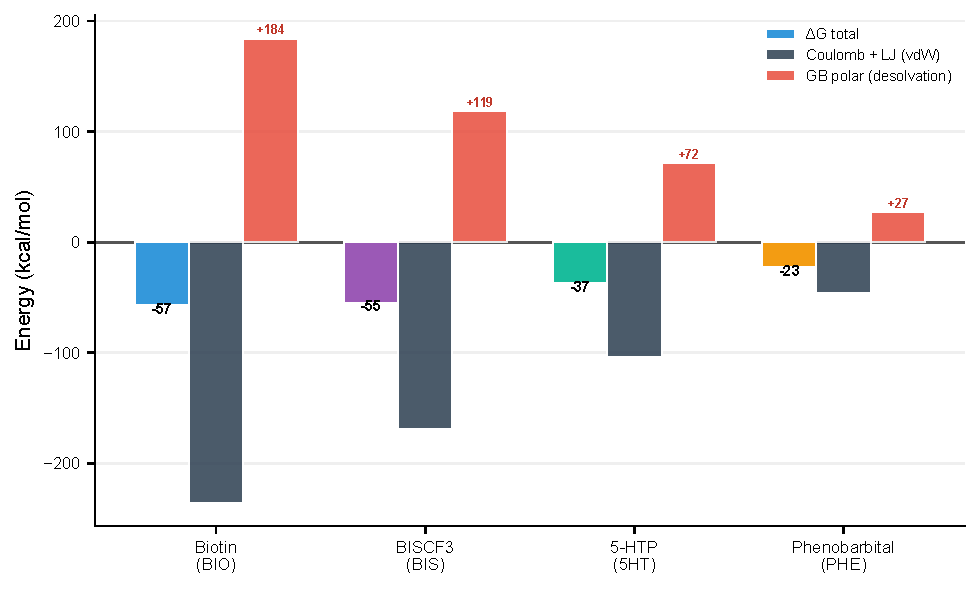
\includegraphics[width=\textwidth]{figures/Fig_MMGBSA_decomposition.pdf}
\caption{MM-GBSA energy decomposition of membrane-bound ligands: $\Delta G$ total, Coulomb + van der Waals, and GB polar desolvation.}
\label{fig:s20}
\end{figure}

\begin{figure}[t]
\centering
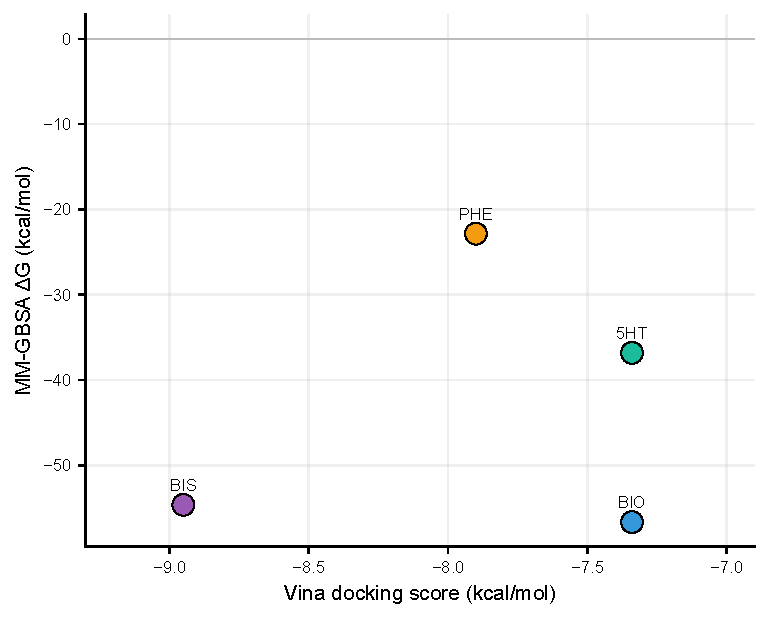
\includegraphics[width=\textwidth]{figures/Fig_docking_vs_MMGBSA.pdf}
\caption{Vina docking vs.\ membrane MM-GBSA cross-validation for the four carboxyl-discriminating ligands.}
\label{fig:s21}
\end{figure}

\begin{figure}[t]
\centering
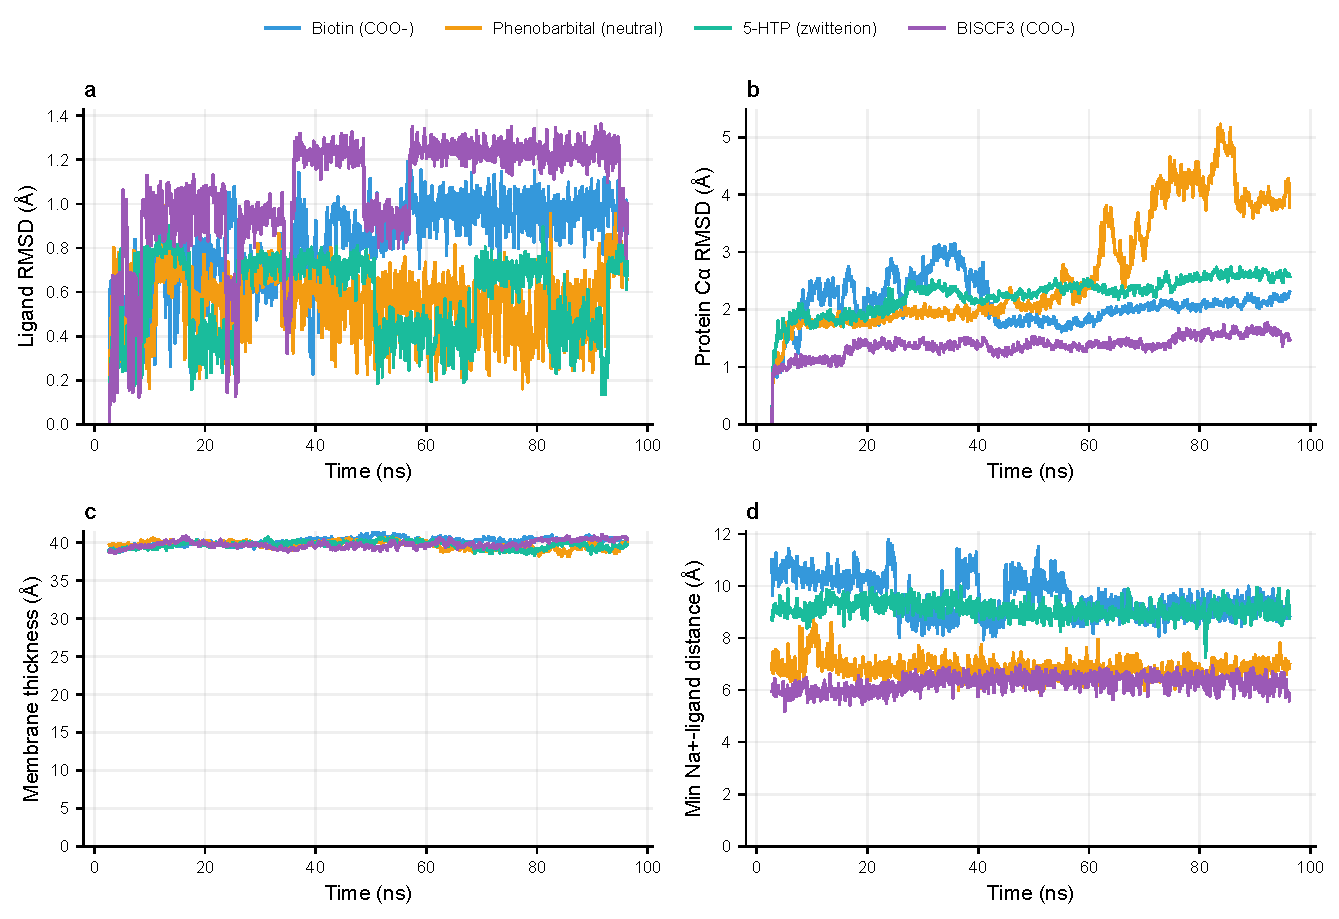
\includegraphics[width=\textwidth]{figures/Fig_BISCF3_MD_stability.pdf}
\caption{Stability of BISCF3 in membrane-embedded Na\textsuperscript{+}-bound MD. Time series over 100~ns for biotin, phenobarbital, 5-HTP, and BISCF3: (a) ligand heavy-atom RMSD, (b) protein C$\alpha$ RMSD, (c) bilayer thickness, and (d) minimum Na\textsuperscript{+}--ligand distance.}
\label{fig:s22}
\end{figure}

\begin{figure}[t]
\centering
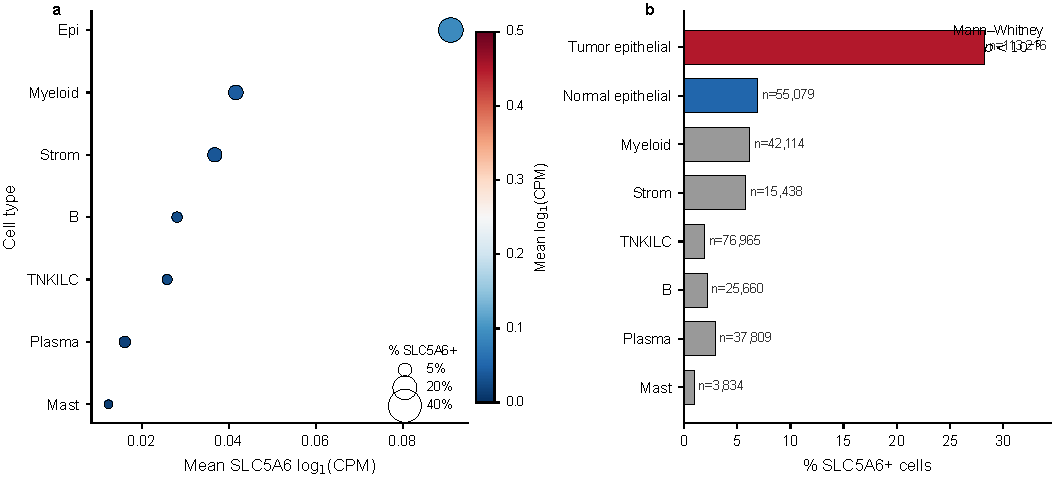
\includegraphics[width=\textwidth]{figures/FigS23_SLC5A6_celltype.pdf}
\caption{SLC5A6 single-cell cell-type localization in colorectal cancer (GSE178341, 370,115 cells). (a) Dot plot of SLC5A6 mean expression (colour) and fraction of positive cells (dot size) across cell types; epithelial cells show the highest detection and mean expression. (b) SLC5A6 expression in tumor versus normal epithelium and the major immune and stromal populations, confirming tumor-epithelial upregulation.}
\label{fig:s23}
\end{figure}

% ═══════════════════════════════════════════════════════════════
% REFERENCES (BibTeX)
% ═══════════════════════════════════════════════════════════════

% sn-jnl sets \bibliographystyle from the sn-nature class option; an explicit
% \bibliographystyle here makes BibTeX abort with "another \bibstyle command".
\bibliography{references}

\end{document}
